\chapter{Phương pháp và thiết kế hệ thống}
\label{ch:phuong-phap}
% Đề mục 4: Biểu diễn game/state/action/reward; kiến trúc engine, agent, UI; thuật toán từng cấp;
% dữ liệu, quy trình train và thiết kế giải đấu công bằng. Nguồn: tài liệu thiết kế Phần 01--09.

\section{Mô hình hoá trò chơi}
\subsection{Trạng thái, hành động, hàm chuyển, phần thưởng}
Trạng thái gồm hai bitboard rời nhau, bên đến lượt, lịch sử, khóa Zobrist và người thắng nếu có. Hành động là chỉ số nguyên từ 0 đến 120 của một ô trống; mỗi hành động đổi bên đến lượt. Sau một nước hợp lệ, engine kiểm tra năm quân liên tiếp của bên vừa đi; khi bàn đầy và chưa có người thắng thì ván hòa. Hàm \texttt{step} trả phần thưởng theo bên vừa đi, còn \texttt{result} trả kết quả theo X. Tách hai quy ước này là điều kiện để huấn luyện value và thống kê W/D/L đúng dấu.
\subsection{Input / output của tác tử}
Tác tử nhận bàn cờ và \texttt{Limits}, rồi trả một chỉ số nước đi. \texttt{reset(seed)} thiết lập lại trạng thái theo ván. \texttt{last\_stats()} trả dữ liệu tùy thuật toán: số nút, độ sâu, phân phối policy, số mô phỏng hoặc biến chính. Mã arena đo thời gian bên ngoài lời gọi tác tử, do đó có cả chi phí sao chép trạng thái mà tác tử nhận.

\section{Kiến trúc hệ thống}
\subsection{Các khối chính và nguyên tắc phụ thuộc}
Các mô-đun tạo thành một đường dữ liệu một chiều: engine định nghĩa luật; tác tử biến trạng thái thành nước đi; arena ghép tác tử và ghi ván; training tái sử dụng engine, tác tử và mạng; giao diện dựng lại trạng thái từ lịch sử. Cấu trúc này cho phép phát lại bằng đúng luật dùng trong thí nghiệm và thay tác tử mà không đổi protocol của ván.
\subsection{Cấu hình, seed và log}
Cấu hình YAML được hợp nhất qua \texttt{defaults} rồi mới áp dụng tham số ghi đè từ dòng lệnh. Seed ván và seed màu được dẫn xuất bằng băm ổn định. Mỗi lượt lưu cấu hình đã hợp nhất, thông tin môi trường, log ván JSONL và tổng kết. Một cấu hình tồn tại chỉ mô tả thiết kế; bằng chứng đã chạy là log có số ván và trạng thái hoàn tất. Hai lượt có cùng tên nhưng khác ngân sách phải được xem là hai phép đo riêng.

\section{Engine bitboard}
\label{sec:engine}
Mọi tác tử, từ luật cứng đến tìm kiếm cây, đều phải hỏi engine hàng nghìn lần mỗi nước: đã có ai thắng chưa, nên xét những ô nào, ô nào thắng ngay, thế cờ đang tốt cho bên nào. Engine trong \texttt{caro/engine/} trả lời các câu hỏi đó bằng phép toán bit trên số nguyên thay vì duyệt mảng hai chiều. Mục này trình bày từng phép tính kèm ví dụ cụ thể. Toàn bộ hình và bảng số liệu trong mục được sinh từ chính code của engine bằng \texttt{report/scripts/ve\_hinh\_bitboard.py}, nên khớp với kết quả chạy thật.

\subsection{Biểu diễn bitboard}
\label{sec:bb-bieu-dien}

\subsubsection{Từ ô cờ sang bit}
Quân của mỗi bên được lưu trong một số nguyên 121 bit, bit bằng 1 nghĩa là ô đó có quân của bên ấy. Ô ở hàng $r$, cột $c$ (đánh số từ 0) ứng với bit
\begin{equation}
  i = 11r + c, \qquad r = \lfloor i / 11 \rfloor, \quad c = i \bmod 11.
  \label{eq:chi-so}
\end{equation}
Hình~\ref{fig:chi-so}a cho thấy chỉ số của cả bàn: bit 0 ở góc trên trái, bit 120 ở góc dưới phải, ô trung tâm $(5, 5)$ là bit 60. Với thế cờ ở Hình~\ref{fig:chi-so}b, X có các ô $(4,4)$, $(5,5)$, $(5,6)$ nên có các bit 48, 60, 61; hai số nguyên tương ứng nằm ở Bảng~\ref{tab:bb-vi-du}.

\begin{figure}[H]
  \centering
  % Sinh tự động bởi report/scripts/ve_hinh_bitboard.py, đừng sửa tay.
\definecolor{bbX}{HTML}{1F4E8C}
\definecolor{bbO}{HTML}{C8553D}
\definecolor{bbKq}{HTML}{2E8B57}
\definecolor{bbSai}{HTML}{D7263D}
\definecolor{bbMat}{HTML}{DCE8F5}
\definecolor{bbVang}{HTML}{FBE7A1}
\definecolor{bbXam}{HTML}{BDBDBD}
\definecolor{bbNhat}{HTML}{9CC3E6}
\begin{tikzpicture}
\fill[bbVang] (3.100,-3.100) rectangle ++(0.620,-0.620);
\fill[bbNhat] (3.720,-3.100) rectangle ++(0.620,-0.620);
\fill[bbNhat] (3.100,-3.720) rectangle ++(0.620,-0.620);
\fill[bbNhat] (3.720,-3.720) rectangle ++(0.620,-0.620);
\fill[bbNhat] (2.480,-3.720) rectangle ++(0.620,-0.620);
\draw[gray!55,line width=.2pt] (0,0) grid[step=0.62] (6.820,-6.820);
\draw[gray!90!black,line width=.5pt] (0,0) rectangle (6.820,-6.820);
\node[font=\fontsize{7}{7}\selectfont] at (0.310,-0.310) {0};
\node[font=\fontsize{7}{7}\selectfont] at (0.930,-0.310) {1};
\node[font=\fontsize{7}{7}\selectfont] at (1.550,-0.310) {2};
\node[font=\fontsize{7}{7}\selectfont] at (2.170,-0.310) {3};
\node[font=\fontsize{7}{7}\selectfont] at (2.790,-0.310) {4};
\node[font=\fontsize{7}{7}\selectfont] at (3.410,-0.310) {5};
\node[font=\fontsize{7}{7}\selectfont] at (4.030,-0.310) {6};
\node[font=\fontsize{7}{7}\selectfont] at (4.650,-0.310) {7};
\node[font=\fontsize{7}{7}\selectfont] at (5.270,-0.310) {8};
\node[font=\fontsize{7}{7}\selectfont] at (5.890,-0.310) {9};
\node[font=\fontsize{7}{7}\selectfont] at (6.510,-0.310) {10};
\node[font=\fontsize{7}{7}\selectfont] at (0.310,-0.930) {11};
\node[font=\fontsize{7}{7}\selectfont] at (0.930,-0.930) {12};
\node[font=\fontsize{7}{7}\selectfont] at (1.550,-0.930) {13};
\node[font=\fontsize{7}{7}\selectfont] at (2.170,-0.930) {14};
\node[font=\fontsize{7}{7}\selectfont] at (2.790,-0.930) {15};
\node[font=\fontsize{7}{7}\selectfont] at (3.410,-0.930) {16};
\node[font=\fontsize{7}{7}\selectfont] at (4.030,-0.930) {17};
\node[font=\fontsize{7}{7}\selectfont] at (4.650,-0.930) {18};
\node[font=\fontsize{7}{7}\selectfont] at (5.270,-0.930) {19};
\node[font=\fontsize{7}{7}\selectfont] at (5.890,-0.930) {20};
\node[font=\fontsize{7}{7}\selectfont] at (6.510,-0.930) {21};
\node[font=\fontsize{7}{7}\selectfont] at (0.310,-1.550) {22};
\node[font=\fontsize{7}{7}\selectfont] at (0.930,-1.550) {23};
\node[font=\fontsize{7}{7}\selectfont] at (1.550,-1.550) {24};
\node[font=\fontsize{7}{7}\selectfont] at (2.170,-1.550) {25};
\node[font=\fontsize{7}{7}\selectfont] at (2.790,-1.550) {26};
\node[font=\fontsize{7}{7}\selectfont] at (3.410,-1.550) {27};
\node[font=\fontsize{7}{7}\selectfont] at (4.030,-1.550) {28};
\node[font=\fontsize{7}{7}\selectfont] at (4.650,-1.550) {29};
\node[font=\fontsize{7}{7}\selectfont] at (5.270,-1.550) {30};
\node[font=\fontsize{7}{7}\selectfont] at (5.890,-1.550) {31};
\node[font=\fontsize{7}{7}\selectfont] at (6.510,-1.550) {32};
\node[font=\fontsize{7}{7}\selectfont] at (0.310,-2.170) {33};
\node[font=\fontsize{7}{7}\selectfont] at (0.930,-2.170) {34};
\node[font=\fontsize{7}{7}\selectfont] at (1.550,-2.170) {35};
\node[font=\fontsize{7}{7}\selectfont] at (2.170,-2.170) {36};
\node[font=\fontsize{7}{7}\selectfont] at (2.790,-2.170) {37};
\node[font=\fontsize{7}{7}\selectfont] at (3.410,-2.170) {38};
\node[font=\fontsize{7}{7}\selectfont] at (4.030,-2.170) {39};
\node[font=\fontsize{7}{7}\selectfont] at (4.650,-2.170) {40};
\node[font=\fontsize{7}{7}\selectfont] at (5.270,-2.170) {41};
\node[font=\fontsize{7}{7}\selectfont] at (5.890,-2.170) {42};
\node[font=\fontsize{7}{7}\selectfont] at (6.510,-2.170) {43};
\node[font=\fontsize{7}{7}\selectfont] at (0.310,-2.790) {44};
\node[font=\fontsize{7}{7}\selectfont] at (0.930,-2.790) {45};
\node[font=\fontsize{7}{7}\selectfont] at (1.550,-2.790) {46};
\node[font=\fontsize{7}{7}\selectfont] at (2.170,-2.790) {47};
\node[font=\fontsize{7}{7}\selectfont] at (2.790,-2.790) {48};
\node[font=\fontsize{7}{7}\selectfont] at (3.410,-2.790) {49};
\node[font=\fontsize{7}{7}\selectfont] at (4.030,-2.790) {50};
\node[font=\fontsize{7}{7}\selectfont] at (4.650,-2.790) {51};
\node[font=\fontsize{7}{7}\selectfont] at (5.270,-2.790) {52};
\node[font=\fontsize{7}{7}\selectfont] at (5.890,-2.790) {53};
\node[font=\fontsize{7}{7}\selectfont] at (6.510,-2.790) {54};
\node[font=\fontsize{7}{7}\selectfont] at (0.310,-3.410) {55};
\node[font=\fontsize{7}{7}\selectfont] at (0.930,-3.410) {56};
\node[font=\fontsize{7}{7}\selectfont] at (1.550,-3.410) {57};
\node[font=\fontsize{7}{7}\selectfont] at (2.170,-3.410) {58};
\node[font=\fontsize{7}{7}\selectfont] at (2.790,-3.410) {59};
\node[font=\fontsize{7}{7}\selectfont] at (3.410,-3.410) {60};
\node[font=\fontsize{7}{7}\selectfont] at (4.030,-3.410) {61};
\node[font=\fontsize{7}{7}\selectfont] at (4.650,-3.410) {62};
\node[font=\fontsize{7}{7}\selectfont] at (5.270,-3.410) {63};
\node[font=\fontsize{7}{7}\selectfont] at (5.890,-3.410) {64};
\node[font=\fontsize{7}{7}\selectfont] at (6.510,-3.410) {65};
\node[font=\fontsize{7}{7}\selectfont] at (0.310,-4.030) {66};
\node[font=\fontsize{7}{7}\selectfont] at (0.930,-4.030) {67};
\node[font=\fontsize{7}{7}\selectfont] at (1.550,-4.030) {68};
\node[font=\fontsize{7}{7}\selectfont] at (2.170,-4.030) {69};
\node[font=\fontsize{7}{7}\selectfont] at (2.790,-4.030) {70};
\node[font=\fontsize{7}{7}\selectfont] at (3.410,-4.030) {71};
\node[font=\fontsize{7}{7}\selectfont] at (4.030,-4.030) {72};
\node[font=\fontsize{7}{7}\selectfont] at (4.650,-4.030) {73};
\node[font=\fontsize{7}{7}\selectfont] at (5.270,-4.030) {74};
\node[font=\fontsize{7}{7}\selectfont] at (5.890,-4.030) {75};
\node[font=\fontsize{7}{7}\selectfont] at (6.510,-4.030) {76};
\node[font=\fontsize{7}{7}\selectfont] at (0.310,-4.650) {77};
\node[font=\fontsize{7}{7}\selectfont] at (0.930,-4.650) {78};
\node[font=\fontsize{7}{7}\selectfont] at (1.550,-4.650) {79};
\node[font=\fontsize{7}{7}\selectfont] at (2.170,-4.650) {80};
\node[font=\fontsize{7}{7}\selectfont] at (2.790,-4.650) {81};
\node[font=\fontsize{7}{7}\selectfont] at (3.410,-4.650) {82};
\node[font=\fontsize{7}{7}\selectfont] at (4.030,-4.650) {83};
\node[font=\fontsize{7}{7}\selectfont] at (4.650,-4.650) {84};
\node[font=\fontsize{7}{7}\selectfont] at (5.270,-4.650) {85};
\node[font=\fontsize{7}{7}\selectfont] at (5.890,-4.650) {86};
\node[font=\fontsize{7}{7}\selectfont] at (6.510,-4.650) {87};
\node[font=\fontsize{7}{7}\selectfont] at (0.310,-5.270) {88};
\node[font=\fontsize{7}{7}\selectfont] at (0.930,-5.270) {89};
\node[font=\fontsize{7}{7}\selectfont] at (1.550,-5.270) {90};
\node[font=\fontsize{7}{7}\selectfont] at (2.170,-5.270) {91};
\node[font=\fontsize{7}{7}\selectfont] at (2.790,-5.270) {92};
\node[font=\fontsize{7}{7}\selectfont] at (3.410,-5.270) {93};
\node[font=\fontsize{7}{7}\selectfont] at (4.030,-5.270) {94};
\node[font=\fontsize{7}{7}\selectfont] at (4.650,-5.270) {95};
\node[font=\fontsize{7}{7}\selectfont] at (5.270,-5.270) {96};
\node[font=\fontsize{7}{7}\selectfont] at (5.890,-5.270) {97};
\node[font=\fontsize{7}{7}\selectfont] at (6.510,-5.270) {98};
\node[font=\fontsize{7}{7}\selectfont] at (0.310,-5.890) {99};
\node[font=\fontsize{7}{7}\selectfont] at (0.930,-5.890) {100};
\node[font=\fontsize{7}{7}\selectfont] at (1.550,-5.890) {101};
\node[font=\fontsize{7}{7}\selectfont] at (2.170,-5.890) {102};
\node[font=\fontsize{7}{7}\selectfont] at (2.790,-5.890) {103};
\node[font=\fontsize{7}{7}\selectfont] at (3.410,-5.890) {104};
\node[font=\fontsize{7}{7}\selectfont] at (4.030,-5.890) {105};
\node[font=\fontsize{7}{7}\selectfont] at (4.650,-5.890) {106};
\node[font=\fontsize{7}{7}\selectfont] at (5.270,-5.890) {107};
\node[font=\fontsize{7}{7}\selectfont] at (5.890,-5.890) {108};
\node[font=\fontsize{7}{7}\selectfont] at (6.510,-5.890) {109};
\node[font=\fontsize{7}{7}\selectfont] at (0.310,-6.510) {110};
\node[font=\fontsize{7}{7}\selectfont] at (0.930,-6.510) {111};
\node[font=\fontsize{7}{7}\selectfont] at (1.550,-6.510) {112};
\node[font=\fontsize{7}{7}\selectfont] at (2.170,-6.510) {113};
\node[font=\fontsize{7}{7}\selectfont] at (2.790,-6.510) {114};
\node[font=\fontsize{7}{7}\selectfont] at (3.410,-6.510) {115};
\node[font=\fontsize{7}{7}\selectfont] at (4.030,-6.510) {116};
\node[font=\fontsize{7}{7}\selectfont] at (4.650,-6.510) {117};
\node[font=\fontsize{7}{7}\selectfont] at (5.270,-6.510) {118};
\node[font=\fontsize{7}{7}\selectfont] at (5.890,-6.510) {119};
\node[font=\fontsize{7}{7}\selectfont] at (6.510,-6.510) {120};
\node[font=\fontsize{7}{7}\selectfont\itshape,gray] at (0.310,.17) {0};
\node[font=\fontsize{7}{7}\selectfont\itshape,gray] at (-.2,-0.310) {0};
\node[font=\fontsize{7}{7}\selectfont\itshape,gray] at (0.930,.17) {1};
\node[font=\fontsize{7}{7}\selectfont\itshape,gray] at (-.2,-0.930) {1};
\node[font=\fontsize{7}{7}\selectfont\itshape,gray] at (1.550,.17) {2};
\node[font=\fontsize{7}{7}\selectfont\itshape,gray] at (-.2,-1.550) {2};
\node[font=\fontsize{7}{7}\selectfont\itshape,gray] at (2.170,.17) {3};
\node[font=\fontsize{7}{7}\selectfont\itshape,gray] at (-.2,-2.170) {3};
\node[font=\fontsize{7}{7}\selectfont\itshape,gray] at (2.790,.17) {4};
\node[font=\fontsize{7}{7}\selectfont\itshape,gray] at (-.2,-2.790) {4};
\node[font=\fontsize{7}{7}\selectfont\itshape,gray] at (3.410,.17) {5};
\node[font=\fontsize{7}{7}\selectfont\itshape,gray] at (-.2,-3.410) {5};
\node[font=\fontsize{7}{7}\selectfont\itshape,gray] at (4.030,.17) {6};
\node[font=\fontsize{7}{7}\selectfont\itshape,gray] at (-.2,-4.030) {6};
\node[font=\fontsize{7}{7}\selectfont\itshape,gray] at (4.650,.17) {7};
\node[font=\fontsize{7}{7}\selectfont\itshape,gray] at (-.2,-4.650) {7};
\node[font=\fontsize{7}{7}\selectfont\itshape,gray] at (5.270,.17) {8};
\node[font=\fontsize{7}{7}\selectfont\itshape,gray] at (-.2,-5.270) {8};
\node[font=\fontsize{7}{7}\selectfont\itshape,gray] at (5.890,.17) {9};
\node[font=\fontsize{7}{7}\selectfont\itshape,gray] at (-.2,-5.890) {9};
\node[font=\fontsize{7}{7}\selectfont\itshape,gray] at (6.510,.17) {10};
\node[font=\fontsize{7}{7}\selectfont\itshape,gray] at (-.2,-6.510) {10};
\node[anchor=south,font=\footnotesize] at (3.410,.32) {(a) Chỉ số bit $i = 11r + c$; từ ô 60 đi 4 hướng};
\begin{scope}[shift={(7.720,0.000)}]
\fill[bbX] (2.480,-2.480) rectangle ++(0.620,-0.620);
\node[text=white,inner sep=0,font=\footnotesize\bfseries] at (2.790,-2.790) {X};
\fill[bbX] (3.100,-3.100) rectangle ++(0.620,-0.620);
\node[text=white,inner sep=0,font=\footnotesize\bfseries] at (3.410,-3.410) {X};
\fill[bbX] (3.720,-3.100) rectangle ++(0.620,-0.620);
\node[text=white,inner sep=0,font=\footnotesize\bfseries] at (4.030,-3.410) {X};
\fill[bbO] (3.720,-2.480) rectangle ++(0.620,-0.620);
\node[text=white,inner sep=0,font=\footnotesize\bfseries] at (4.030,-2.790) {O};
\fill[bbO] (2.480,-3.720) rectangle ++(0.620,-0.620);
\node[text=white,inner sep=0,font=\footnotesize\bfseries] at (2.790,-4.030) {O};
\draw[gray!55,line width=.2pt] (0,0) grid[step=0.620] (6.820,-6.820);
\draw[gray!90!black,line width=.5pt] (0,0) rectangle (6.820,-6.820);
\node[font=\fontsize{5}{5}\selectfont,gray] at (0.310,.09) {0};
\node[font=\fontsize{5}{5}\selectfont,gray] at (-.12,-0.310) {0};
\node[font=\fontsize{5}{5}\selectfont,gray] at (0.930,.09) {1};
\node[font=\fontsize{5}{5}\selectfont,gray] at (-.12,-0.930) {1};
\node[font=\fontsize{5}{5}\selectfont,gray] at (1.550,.09) {2};
\node[font=\fontsize{5}{5}\selectfont,gray] at (-.12,-1.550) {2};
\node[font=\fontsize{5}{5}\selectfont,gray] at (2.170,.09) {3};
\node[font=\fontsize{5}{5}\selectfont,gray] at (-.12,-2.170) {3};
\node[font=\fontsize{5}{5}\selectfont,gray] at (2.790,.09) {4};
\node[font=\fontsize{5}{5}\selectfont,gray] at (-.12,-2.790) {4};
\node[font=\fontsize{5}{5}\selectfont,gray] at (3.410,.09) {5};
\node[font=\fontsize{5}{5}\selectfont,gray] at (-.12,-3.410) {5};
\node[font=\fontsize{5}{5}\selectfont,gray] at (4.030,.09) {6};
\node[font=\fontsize{5}{5}\selectfont,gray] at (-.12,-4.030) {6};
\node[font=\fontsize{5}{5}\selectfont,gray] at (4.650,.09) {7};
\node[font=\fontsize{5}{5}\selectfont,gray] at (-.12,-4.650) {7};
\node[font=\fontsize{5}{5}\selectfont,gray] at (5.270,.09) {8};
\node[font=\fontsize{5}{5}\selectfont,gray] at (-.12,-5.270) {8};
\node[font=\fontsize{5}{5}\selectfont,gray] at (5.890,.09) {9};
\node[font=\fontsize{5}{5}\selectfont,gray] at (-.12,-5.890) {9};
\node[font=\fontsize{5}{5}\selectfont,gray] at (6.510,.09) {10};
\node[font=\fontsize{5}{5}\selectfont,gray] at (-.12,-6.510) {10};
\node[anchor=south,font=\footnotesize] at (3.410,0.16) {(b) Thế cờ ví dụ};
\end{scope}
\end{tikzpicture}

  \caption{Đánh số 121 ô thành 121 bit và thế cờ dùng làm ví dụ.}
  \label{fig:chi-so}
\end{figure}

\begin{table}[H]
  \centering\small
  \caption{Hai bitboard của thế cờ ở Hình~\ref{fig:chi-so}b.}
  \label{tab:bb-vi-du}
  % Sinh tự động bởi report/scripts/ve_hinh_bitboard.py, đừng sửa tay.
\begin{tabular}{@{}lll@{}}
\toprule
\textbf{Bên} & \textbf{Giá trị số nguyên} & \textbf{Dạng hexa} \\
\midrule
X & $2^{48} + 2^{60} + 2^{61}$ & \texttt{0x3001000000000000} \\
O & $2^{50} + 2^{70}$ & \texttt{0x400004000000000000} \\
\bottomrule
\end{tabular}

\end{table}

Các thao tác cơ bản chỉ cần một phép bit, với \texttt{FULL} $= 2^{121} - 1$:
\begin{itemize}
  \item Đặt quân vào ô $i$: $x \leftarrow x \mid (1 \ll i)$.
  \item Hỏi ô $i$ có quân không: $(x \gg i) \mathbin{\&} 1$.
  \item Các ô đã có quân: $x \mid o$. Các ô trống: $\lnot(x \mid o) \mathbin{\&} \texttt{FULL}$.
\end{itemize}
Phép AND với \texttt{FULL} là cần thiết vì số nguyên Python không giới hạn độ dài: $\lnot y$ cho ra số âm, về mặt logic có vô số bit 1 ở phía cao. Bản C++/Rust có thể dùng kiểu \texttt{u128} với cùng công thức, chỉ còn 7 bit cao thừa.

\subsubsection{Liệt kê các bit 1}
Hàm \texttt{iter\_bits} biến bitboard thành danh sách ô theo thứ tự tăng dần. Trong biểu diễn bù 2, $-b$ đảo mọi bit phía trên bit 1 thấp nhất và giữ nguyên bit đó, nên $b \mathbin{\&} -b$ tách đúng bit này ra. Bảng~\ref{tab:iter-bits} chạy thử với $b = 104 = 1101000_2$: ba vòng lặp cho ba chỉ số 3, 5, 6. Số vòng lặp bằng số bit 1, không phụ thuộc kích thước bàn.

\begin{table}[H]
  \centering\small
  \caption{Các bước của \texttt{iter\_bits} với $b = 104$.}
  \label{tab:iter-bits}
  % Sinh tự động bởi report/scripts/ve_hinh_bitboard.py, đừng sửa tay.
\begin{tabular}{@{}ccccc@{}}
\toprule
$b$ & $-b$ (bù 2, 8 bit thấp) & $low = b \mathbin{\&} -b$ & \textbf{Chỉ số} & $b \oplus low$ \\
\midrule
\texttt{01101000} & \texttt{10011000} & \texttt{00001000} & 3 & \texttt{01100000} \\
\texttt{01100000} & \texttt{10100000} & \texttt{00100000} & 5 & \texttt{01000000} \\
\texttt{01000000} & \texttt{11000000} & \texttt{01000000} & 6 & \texttt{00000000} \\
\bottomrule
\end{tabular}

\end{table}

\subsubsection{Dịch bit là đi theo một hướng}
Theo công thức~\eqref{eq:chi-so}, đi một bước $(\Delta r, \Delta c)$ làm chỉ số tăng $d = 11\Delta r + \Delta c$. Vì vậy bốn hướng của bàn cờ ứng với bốn độ dịch (Bảng~\ref{tab:huong}). Bốn hướng này đủ để xét mọi dãy, vì chiều ngược lại chỉ là cùng một dãy nhìn từ đầu kia.

\begin{table}[H]
  \centering\small
  \caption{Bốn hướng và độ dịch tương ứng.}
  \label{tab:huong}
  \begin{tabular}{@{}lccc@{}}
    \toprule
    \textbf{Hướng} & $(\Delta r, \Delta c)$ & \textbf{Độ dịch} $d$ & \textbf{Từ ô 60 tới ô} \\
    \midrule
    Ngang $\rightarrow$ & $(0, 1)$ & 1 & 61 \\
    Dọc $\downarrow$ & $(1, 0)$ & 11 & 71 \\
    Chéo $\searrow$ & $(1, 1)$ & 12 & 72 \\
    Chéo $\swarrow$ & $(1, -1)$ & 10 & 70 \\
    \bottomrule
  \end{tabular}
\end{table}

Tính chất mà mọi thuật toán phía sau dựa vào là:
\begin{equation}
  \text{bit } i \text{ của } (x \gg d) \;=\; \text{bit } (i + d) \text{ của } x.
  \label{eq:dich}
\end{equation}
Nghĩa là $x \gg d$ trả lời cùng lúc cho cả 121 ô câu hỏi ``đi một bước theo hướng $d$ có gặp quân không?''. Trên hình, cả bàn trượt ngược hướng $d$ một bước (Hình~\ref{fig:dich-bit}).

\begin{figure}[H]
  \centering
  % Sinh tự động bởi report/scripts/ve_hinh_bitboard.py, đừng sửa tay.
\definecolor{bbX}{HTML}{1F4E8C}
\definecolor{bbO}{HTML}{C8553D}
\definecolor{bbKq}{HTML}{2E8B57}
\definecolor{bbSai}{HTML}{D7263D}
\definecolor{bbMat}{HTML}{DCE8F5}
\definecolor{bbVang}{HTML}{FBE7A1}
\definecolor{bbXam}{HTML}{BDBDBD}
\definecolor{bbNhat}{HTML}{9CC3E6}
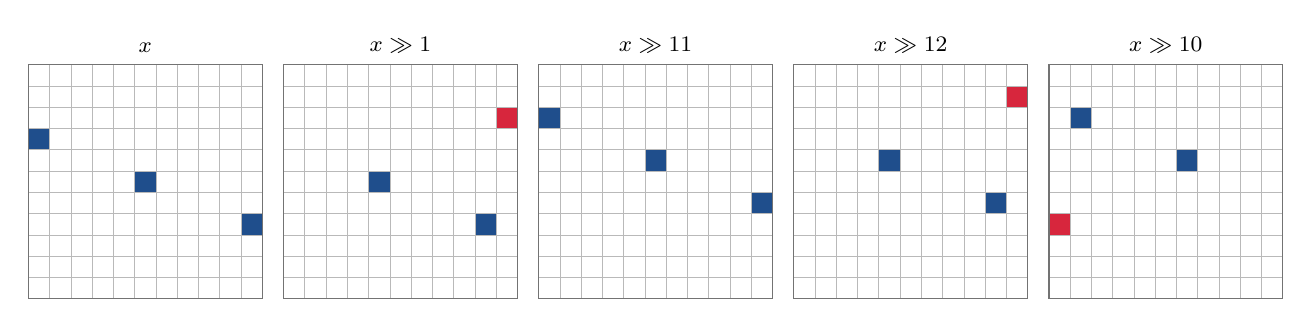
\begin{tikzpicture}
\begin{scope}[shift={(0.000,0.000)}]
\fill[bbX] (0.000,-0.810) rectangle ++(0.270,-0.270);
\fill[bbX] (1.350,-1.350) rectangle ++(0.270,-0.270);
\fill[bbX] (2.700,-1.890) rectangle ++(0.270,-0.270);
\draw[gray!55,line width=.2pt] (0,0) grid[step=0.270] (2.970,-2.970);
\draw[gray!90!black,line width=.5pt] (0,0) rectangle (2.970,-2.970);
\node[anchor=south,font=\footnotesize] at (1.485,0.03) {$x$};
\end{scope}
\begin{scope}[shift={(3.240,0.000)}]
\fill[bbX] (1.080,-1.350) rectangle ++(0.270,-0.270);
\fill[bbX] (2.430,-1.890) rectangle ++(0.270,-0.270);
\fill[bbSai] (2.700,-0.540) rectangle ++(0.270,-0.270);
\draw[gray!55,line width=.2pt] (0,0) grid[step=0.270] (2.970,-2.970);
\draw[gray!90!black,line width=.5pt] (0,0) rectangle (2.970,-2.970);
\node[anchor=south,font=\footnotesize] at (1.485,0.03) {$x \gg 1$};
\end{scope}
\begin{scope}[shift={(6.480,0.000)}]
\fill[bbX] (0.000,-0.540) rectangle ++(0.270,-0.270);
\fill[bbX] (1.350,-1.080) rectangle ++(0.270,-0.270);
\fill[bbX] (2.700,-1.620) rectangle ++(0.270,-0.270);
\draw[gray!55,line width=.2pt] (0,0) grid[step=0.270] (2.970,-2.970);
\draw[gray!90!black,line width=.5pt] (0,0) rectangle (2.970,-2.970);
\node[anchor=south,font=\footnotesize] at (1.485,0.03) {$x \gg 11$};
\end{scope}
\begin{scope}[shift={(9.720,0.000)}]
\fill[bbX] (1.080,-1.080) rectangle ++(0.270,-0.270);
\fill[bbX] (2.430,-1.620) rectangle ++(0.270,-0.270);
\fill[bbSai] (2.700,-0.270) rectangle ++(0.270,-0.270);
\draw[gray!55,line width=.2pt] (0,0) grid[step=0.270] (2.970,-2.970);
\draw[gray!90!black,line width=.5pt] (0,0) rectangle (2.970,-2.970);
\node[anchor=south,font=\footnotesize] at (1.485,0.03) {$x \gg 12$};
\end{scope}
\begin{scope}[shift={(12.960,0.000)}]
\fill[bbX] (0.270,-0.540) rectangle ++(0.270,-0.270);
\fill[bbX] (1.620,-1.080) rectangle ++(0.270,-0.270);
\fill[bbSai] (0.000,-1.890) rectangle ++(0.270,-0.270);
\draw[gray!55,line width=.2pt] (0,0) grid[step=0.270] (2.970,-2.970);
\draw[gray!90!black,line width=.5pt] (0,0) rectangle (2.970,-2.970);
\node[anchor=south,font=\footnotesize] at (1.485,0.03) {$x \gg 10$};
\end{scope}
\end{tikzpicture}

  \caption{Tác dụng của phép dịch lên ba quân $(5,5)$, $(3,0)$, $(7,10)$. Ô đỏ là kết quả lọt hàng.}
  \label{fig:dich-bit}
\end{figure}

Các ô đỏ trong Hình~\ref{fig:dich-bit} cho thấy cái bẫy của cách xếp này. Mỗi hàng rộng đúng 11 bit, không có cột đệm, nên quân ở mép bàn có thể ``lọt'' sang hàng khác. Chẳng hạn $x \gg 1$ đưa quân $(3, 0)$, bit 33, về bit 32, tức ô $(2, 10)$ ở cuối hàng trên, dù hai ô này không kề nhau trên bàn. Tương tự, $x \gg 10$ đưa quân $(7, 10)$, bit 87, về bit 77, tức ô $(7, 0)$ ở đầu cùng hàng.

\subsubsection{Mặt nạ START}
Để loại kết quả lọt hàng, mỗi hướng có một mặt nạ gồm những ô được phép là ô đầu của một dãy 5 nằm trọn trong bàn:
\begin{equation}
  \mathrm{START}_d = \{(r, c) : 0 \le r + 4\Delta r \le 10 \;\text{ và }\; 0 \le c + 4\Delta c \le 10\}.
  \label{eq:start}
\end{equation}
Áp dụng công thức ta có ô đầu dãy ngang phải có $c \le 6$, dãy dọc có $r \le 6$, chéo $\searrow$ có $r \le 6, c \le 6$, chéo $\swarrow$ có $r \le 6, c \ge 4$. Số ô lần lượt là $11 \times 7 = 77$, $7 \times 11 = 77$, $7 \times 7 = 49$ và $49$, nên cả bàn có đúng 252 cửa sổ 5 ô (Hình~\ref{fig:start}). Các mặt nạ được sinh bằng vòng lặp khi nạp module, không chép tay hằng số.

\begin{figure}[H]
  \centering
  % Sinh tự động bởi report/scripts/ve_hinh_bitboard.py, đừng sửa tay.
\definecolor{bbX}{HTML}{1F4E8C}
\definecolor{bbO}{HTML}{C8553D}
\definecolor{bbKq}{HTML}{2E8B57}
\definecolor{bbSai}{HTML}{D7263D}
\definecolor{bbMat}{HTML}{DCE8F5}
\definecolor{bbVang}{HTML}{FBE7A1}
\definecolor{bbXam}{HTML}{BDBDBD}
\definecolor{bbNhat}{HTML}{9CC3E6}
\begin{tikzpicture}
\begin{scope}[shift={(0.000,0.000)}]
\fill[bbMat] (0.000,0.000) rectangle ++(0.310,-0.310);
\fill[bbMat] (0.310,0.000) rectangle ++(0.310,-0.310);
\fill[bbMat] (0.620,0.000) rectangle ++(0.310,-0.310);
\fill[bbMat] (0.930,0.000) rectangle ++(0.310,-0.310);
\fill[bbMat] (1.240,0.000) rectangle ++(0.310,-0.310);
\fill[bbMat] (1.550,0.000) rectangle ++(0.310,-0.310);
\fill[bbMat] (1.860,0.000) rectangle ++(0.310,-0.310);
\fill[bbMat] (0.000,-0.310) rectangle ++(0.310,-0.310);
\fill[bbMat] (0.310,-0.310) rectangle ++(0.310,-0.310);
\fill[bbMat] (0.620,-0.310) rectangle ++(0.310,-0.310);
\fill[bbMat] (0.930,-0.310) rectangle ++(0.310,-0.310);
\fill[bbMat] (1.240,-0.310) rectangle ++(0.310,-0.310);
\fill[bbMat] (1.550,-0.310) rectangle ++(0.310,-0.310);
\fill[bbMat] (1.860,-0.310) rectangle ++(0.310,-0.310);
\fill[bbMat] (0.000,-0.620) rectangle ++(0.310,-0.310);
\fill[bbMat] (0.310,-0.620) rectangle ++(0.310,-0.310);
\fill[bbMat] (0.620,-0.620) rectangle ++(0.310,-0.310);
\fill[bbMat] (0.930,-0.620) rectangle ++(0.310,-0.310);
\fill[bbMat] (1.240,-0.620) rectangle ++(0.310,-0.310);
\fill[bbMat] (1.550,-0.620) rectangle ++(0.310,-0.310);
\fill[bbX] (1.860,-0.620) rectangle ++(0.310,-0.310);
\node[text=white,inner sep=0,font=\fontsize{5}{5}\selectfont] at (2.015,-0.775) {28};
\fill[bbMat] (0.000,-0.930) rectangle ++(0.310,-0.310);
\fill[bbMat] (0.310,-0.930) rectangle ++(0.310,-0.310);
\fill[bbMat] (0.620,-0.930) rectangle ++(0.310,-0.310);
\fill[bbMat] (0.930,-0.930) rectangle ++(0.310,-0.310);
\fill[bbMat] (1.240,-0.930) rectangle ++(0.310,-0.310);
\fill[bbMat] (1.550,-0.930) rectangle ++(0.310,-0.310);
\fill[bbMat] (1.860,-0.930) rectangle ++(0.310,-0.310);
\fill[bbMat] (0.000,-1.240) rectangle ++(0.310,-0.310);
\fill[bbMat] (0.310,-1.240) rectangle ++(0.310,-0.310);
\fill[bbMat] (0.620,-1.240) rectangle ++(0.310,-0.310);
\fill[bbMat] (0.930,-1.240) rectangle ++(0.310,-0.310);
\fill[bbMat] (1.240,-1.240) rectangle ++(0.310,-0.310);
\fill[bbMat] (1.550,-1.240) rectangle ++(0.310,-0.310);
\fill[bbMat] (1.860,-1.240) rectangle ++(0.310,-0.310);
\fill[bbMat] (0.000,-1.550) rectangle ++(0.310,-0.310);
\fill[bbMat] (0.310,-1.550) rectangle ++(0.310,-0.310);
\fill[bbMat] (0.620,-1.550) rectangle ++(0.310,-0.310);
\fill[bbMat] (0.930,-1.550) rectangle ++(0.310,-0.310);
\fill[bbMat] (1.240,-1.550) rectangle ++(0.310,-0.310);
\fill[bbMat] (1.550,-1.550) rectangle ++(0.310,-0.310);
\fill[bbMat] (1.860,-1.550) rectangle ++(0.310,-0.310);
\fill[bbMat] (0.000,-1.860) rectangle ++(0.310,-0.310);
\fill[bbMat] (0.310,-1.860) rectangle ++(0.310,-0.310);
\fill[bbMat] (0.620,-1.860) rectangle ++(0.310,-0.310);
\fill[bbMat] (0.930,-1.860) rectangle ++(0.310,-0.310);
\fill[bbMat] (1.240,-1.860) rectangle ++(0.310,-0.310);
\fill[bbMat] (1.550,-1.860) rectangle ++(0.310,-0.310);
\fill[bbMat] (1.860,-1.860) rectangle ++(0.310,-0.310);
\fill[bbMat] (0.000,-2.170) rectangle ++(0.310,-0.310);
\fill[bbMat] (0.310,-2.170) rectangle ++(0.310,-0.310);
\fill[bbMat] (0.620,-2.170) rectangle ++(0.310,-0.310);
\fill[bbMat] (0.930,-2.170) rectangle ++(0.310,-0.310);
\fill[bbMat] (1.240,-2.170) rectangle ++(0.310,-0.310);
\fill[bbMat] (1.550,-2.170) rectangle ++(0.310,-0.310);
\fill[bbMat] (1.860,-2.170) rectangle ++(0.310,-0.310);
\fill[bbMat] (0.000,-2.480) rectangle ++(0.310,-0.310);
\fill[bbMat] (0.310,-2.480) rectangle ++(0.310,-0.310);
\fill[bbMat] (0.620,-2.480) rectangle ++(0.310,-0.310);
\fill[bbMat] (0.930,-2.480) rectangle ++(0.310,-0.310);
\fill[bbMat] (1.240,-2.480) rectangle ++(0.310,-0.310);
\fill[bbMat] (1.550,-2.480) rectangle ++(0.310,-0.310);
\fill[bbMat] (1.860,-2.480) rectangle ++(0.310,-0.310);
\fill[bbMat] (0.000,-2.790) rectangle ++(0.310,-0.310);
\fill[bbMat] (0.310,-2.790) rectangle ++(0.310,-0.310);
\fill[bbMat] (0.620,-2.790) rectangle ++(0.310,-0.310);
\fill[bbMat] (0.930,-2.790) rectangle ++(0.310,-0.310);
\fill[bbMat] (1.240,-2.790) rectangle ++(0.310,-0.310);
\fill[bbMat] (1.550,-2.790) rectangle ++(0.310,-0.310);
\fill[bbMat] (1.860,-2.790) rectangle ++(0.310,-0.310);
\fill[bbMat] (0.000,-3.100) rectangle ++(0.310,-0.310);
\fill[bbMat] (0.310,-3.100) rectangle ++(0.310,-0.310);
\fill[bbMat] (0.620,-3.100) rectangle ++(0.310,-0.310);
\fill[bbMat] (0.930,-3.100) rectangle ++(0.310,-0.310);
\fill[bbMat] (1.240,-3.100) rectangle ++(0.310,-0.310);
\fill[bbMat] (1.550,-3.100) rectangle ++(0.310,-0.310);
\fill[bbMat] (1.860,-3.100) rectangle ++(0.310,-0.310);
\fill[bbX] (2.170,-0.620) rectangle ++(0.310,-0.310);
\node[text=white,inner sep=0,font=\fontsize{5}{5}\selectfont] at (2.325,-0.775) {29};
\fill[bbX] (2.480,-0.620) rectangle ++(0.310,-0.310);
\node[text=white,inner sep=0,font=\fontsize{5}{5}\selectfont] at (2.635,-0.775) {30};
\fill[bbX] (2.790,-0.620) rectangle ++(0.310,-0.310);
\node[text=white,inner sep=0,font=\fontsize{5}{5}\selectfont] at (2.945,-0.775) {31};
\fill[bbX] (3.100,-0.620) rectangle ++(0.310,-0.310);
\node[text=white,inner sep=0,font=\fontsize{5}{5}\selectfont] at (3.255,-0.775) {32};
\draw[gray!55,line width=.2pt] (0,0) grid[step=0.310] (3.410,-3.410);
\draw[gray!90!black,line width=.5pt] (0,0) rectangle (3.410,-3.410);
\node[anchor=south,font=\footnotesize] at (1.705,0.03) {ngang, $d=1$: 77 ô};
\end{scope}
\begin{scope}[shift={(4.060,0.000)}]
\fill[bbMat] (0.000,0.000) rectangle ++(0.310,-0.310);
\fill[bbMat] (0.310,0.000) rectangle ++(0.310,-0.310);
\fill[bbMat] (0.620,0.000) rectangle ++(0.310,-0.310);
\fill[bbMat] (0.930,0.000) rectangle ++(0.310,-0.310);
\fill[bbMat] (1.240,0.000) rectangle ++(0.310,-0.310);
\fill[bbMat] (1.550,0.000) rectangle ++(0.310,-0.310);
\fill[bbMat] (1.860,0.000) rectangle ++(0.310,-0.310);
\fill[bbMat] (2.170,0.000) rectangle ++(0.310,-0.310);
\fill[bbMat] (2.480,0.000) rectangle ++(0.310,-0.310);
\fill[bbMat] (2.790,0.000) rectangle ++(0.310,-0.310);
\fill[bbMat] (3.100,0.000) rectangle ++(0.310,-0.310);
\fill[bbMat] (0.000,-0.310) rectangle ++(0.310,-0.310);
\fill[bbMat] (0.310,-0.310) rectangle ++(0.310,-0.310);
\fill[bbMat] (0.620,-0.310) rectangle ++(0.310,-0.310);
\fill[bbMat] (0.930,-0.310) rectangle ++(0.310,-0.310);
\fill[bbMat] (1.240,-0.310) rectangle ++(0.310,-0.310);
\fill[bbMat] (1.550,-0.310) rectangle ++(0.310,-0.310);
\fill[bbMat] (1.860,-0.310) rectangle ++(0.310,-0.310);
\fill[bbMat] (2.170,-0.310) rectangle ++(0.310,-0.310);
\fill[bbMat] (2.480,-0.310) rectangle ++(0.310,-0.310);
\fill[bbMat] (2.790,-0.310) rectangle ++(0.310,-0.310);
\fill[bbMat] (3.100,-0.310) rectangle ++(0.310,-0.310);
\fill[bbMat] (0.000,-0.620) rectangle ++(0.310,-0.310);
\fill[bbMat] (0.310,-0.620) rectangle ++(0.310,-0.310);
\fill[bbMat] (0.620,-0.620) rectangle ++(0.310,-0.310);
\fill[bbMat] (0.930,-0.620) rectangle ++(0.310,-0.310);
\fill[bbMat] (1.240,-0.620) rectangle ++(0.310,-0.310);
\fill[bbMat] (1.550,-0.620) rectangle ++(0.310,-0.310);
\fill[bbMat] (1.860,-0.620) rectangle ++(0.310,-0.310);
\fill[bbMat] (2.170,-0.620) rectangle ++(0.310,-0.310);
\fill[bbMat] (2.480,-0.620) rectangle ++(0.310,-0.310);
\fill[bbMat] (2.790,-0.620) rectangle ++(0.310,-0.310);
\fill[bbMat] (3.100,-0.620) rectangle ++(0.310,-0.310);
\fill[bbMat] (0.000,-0.930) rectangle ++(0.310,-0.310);
\fill[bbMat] (0.310,-0.930) rectangle ++(0.310,-0.310);
\fill[bbMat] (0.620,-0.930) rectangle ++(0.310,-0.310);
\fill[bbMat] (0.930,-0.930) rectangle ++(0.310,-0.310);
\fill[bbMat] (1.240,-0.930) rectangle ++(0.310,-0.310);
\fill[bbMat] (1.550,-0.930) rectangle ++(0.310,-0.310);
\fill[bbMat] (1.860,-0.930) rectangle ++(0.310,-0.310);
\fill[bbMat] (2.170,-0.930) rectangle ++(0.310,-0.310);
\fill[bbMat] (2.480,-0.930) rectangle ++(0.310,-0.310);
\fill[bbMat] (2.790,-0.930) rectangle ++(0.310,-0.310);
\fill[bbMat] (3.100,-0.930) rectangle ++(0.310,-0.310);
\fill[bbMat] (0.000,-1.240) rectangle ++(0.310,-0.310);
\fill[bbMat] (0.310,-1.240) rectangle ++(0.310,-0.310);
\fill[bbMat] (0.620,-1.240) rectangle ++(0.310,-0.310);
\fill[bbMat] (0.930,-1.240) rectangle ++(0.310,-0.310);
\fill[bbMat] (1.240,-1.240) rectangle ++(0.310,-0.310);
\fill[bbMat] (1.550,-1.240) rectangle ++(0.310,-0.310);
\fill[bbMat] (1.860,-1.240) rectangle ++(0.310,-0.310);
\fill[bbMat] (2.170,-1.240) rectangle ++(0.310,-0.310);
\fill[bbMat] (2.480,-1.240) rectangle ++(0.310,-0.310);
\fill[bbMat] (2.790,-1.240) rectangle ++(0.310,-0.310);
\fill[bbMat] (3.100,-1.240) rectangle ++(0.310,-0.310);
\fill[bbMat] (0.000,-1.550) rectangle ++(0.310,-0.310);
\fill[bbMat] (0.310,-1.550) rectangle ++(0.310,-0.310);
\fill[bbMat] (0.620,-1.550) rectangle ++(0.310,-0.310);
\fill[bbMat] (0.930,-1.550) rectangle ++(0.310,-0.310);
\fill[bbMat] (1.240,-1.550) rectangle ++(0.310,-0.310);
\fill[bbMat] (1.550,-1.550) rectangle ++(0.310,-0.310);
\fill[bbMat] (1.860,-1.550) rectangle ++(0.310,-0.310);
\fill[bbMat] (2.170,-1.550) rectangle ++(0.310,-0.310);
\fill[bbMat] (2.480,-1.550) rectangle ++(0.310,-0.310);
\fill[bbMat] (2.790,-1.550) rectangle ++(0.310,-0.310);
\fill[bbMat] (3.100,-1.550) rectangle ++(0.310,-0.310);
\fill[bbMat] (0.000,-1.860) rectangle ++(0.310,-0.310);
\fill[bbMat] (0.310,-1.860) rectangle ++(0.310,-0.310);
\fill[bbMat] (0.620,-1.860) rectangle ++(0.310,-0.310);
\fill[bbX] (0.930,-1.860) rectangle ++(0.310,-0.310);
\node[text=white,inner sep=0,font=\fontsize{5}{5}\selectfont] at (1.085,-2.015) {69};
\fill[bbMat] (1.240,-1.860) rectangle ++(0.310,-0.310);
\fill[bbMat] (1.550,-1.860) rectangle ++(0.310,-0.310);
\fill[bbMat] (1.860,-1.860) rectangle ++(0.310,-0.310);
\fill[bbMat] (2.170,-1.860) rectangle ++(0.310,-0.310);
\fill[bbMat] (2.480,-1.860) rectangle ++(0.310,-0.310);
\fill[bbMat] (2.790,-1.860) rectangle ++(0.310,-0.310);
\fill[bbMat] (3.100,-1.860) rectangle ++(0.310,-0.310);
\fill[bbX] (0.930,-2.170) rectangle ++(0.310,-0.310);
\node[text=white,inner sep=0,font=\fontsize{5}{5}\selectfont] at (1.085,-2.325) {80};
\fill[bbX] (0.930,-2.480) rectangle ++(0.310,-0.310);
\node[text=white,inner sep=0,font=\fontsize{5}{5}\selectfont] at (1.085,-2.635) {91};
\fill[bbX] (0.930,-2.790) rectangle ++(0.310,-0.310);
\node[text=white,inner sep=0,font=\fontsize{5}{5}\selectfont] at (1.085,-2.945) {102};
\fill[bbX] (0.930,-3.100) rectangle ++(0.310,-0.310);
\node[text=white,inner sep=0,font=\fontsize{5}{5}\selectfont] at (1.085,-3.255) {113};
\draw[gray!55,line width=.2pt] (0,0) grid[step=0.310] (3.410,-3.410);
\draw[gray!90!black,line width=.5pt] (0,0) rectangle (3.410,-3.410);
\node[anchor=south,font=\footnotesize] at (1.705,0.03) {dọc, $d=11$: 77 ô};
\end{scope}
\begin{scope}[shift={(8.120,0.000)}]
\fill[bbMat] (0.000,0.000) rectangle ++(0.310,-0.310);
\fill[bbMat] (0.310,0.000) rectangle ++(0.310,-0.310);
\fill[bbMat] (0.620,0.000) rectangle ++(0.310,-0.310);
\fill[bbMat] (0.930,0.000) rectangle ++(0.310,-0.310);
\fill[bbMat] (1.240,0.000) rectangle ++(0.310,-0.310);
\fill[bbMat] (1.550,0.000) rectangle ++(0.310,-0.310);
\fill[bbMat] (1.860,0.000) rectangle ++(0.310,-0.310);
\fill[bbMat] (0.000,-0.310) rectangle ++(0.310,-0.310);
\fill[bbMat] (0.310,-0.310) rectangle ++(0.310,-0.310);
\fill[bbMat] (0.620,-0.310) rectangle ++(0.310,-0.310);
\fill[bbMat] (0.930,-0.310) rectangle ++(0.310,-0.310);
\fill[bbMat] (1.240,-0.310) rectangle ++(0.310,-0.310);
\fill[bbMat] (1.550,-0.310) rectangle ++(0.310,-0.310);
\fill[bbMat] (1.860,-0.310) rectangle ++(0.310,-0.310);
\fill[bbMat] (0.000,-0.620) rectangle ++(0.310,-0.310);
\fill[bbMat] (0.310,-0.620) rectangle ++(0.310,-0.310);
\fill[bbMat] (0.620,-0.620) rectangle ++(0.310,-0.310);
\fill[bbMat] (0.930,-0.620) rectangle ++(0.310,-0.310);
\fill[bbMat] (1.240,-0.620) rectangle ++(0.310,-0.310);
\fill[bbMat] (1.550,-0.620) rectangle ++(0.310,-0.310);
\fill[bbMat] (1.860,-0.620) rectangle ++(0.310,-0.310);
\fill[bbMat] (0.000,-0.930) rectangle ++(0.310,-0.310);
\fill[bbMat] (0.310,-0.930) rectangle ++(0.310,-0.310);
\fill[bbMat] (0.620,-0.930) rectangle ++(0.310,-0.310);
\fill[bbMat] (0.930,-0.930) rectangle ++(0.310,-0.310);
\fill[bbMat] (1.240,-0.930) rectangle ++(0.310,-0.310);
\fill[bbX] (1.550,-0.930) rectangle ++(0.310,-0.310);
\node[text=white,inner sep=0,font=\fontsize{5}{5}\selectfont] at (1.705,-1.085) {38};
\fill[bbMat] (1.860,-0.930) rectangle ++(0.310,-0.310);
\fill[bbMat] (0.000,-1.240) rectangle ++(0.310,-0.310);
\fill[bbMat] (0.310,-1.240) rectangle ++(0.310,-0.310);
\fill[bbMat] (0.620,-1.240) rectangle ++(0.310,-0.310);
\fill[bbMat] (0.930,-1.240) rectangle ++(0.310,-0.310);
\fill[bbMat] (1.240,-1.240) rectangle ++(0.310,-0.310);
\fill[bbMat] (1.550,-1.240) rectangle ++(0.310,-0.310);
\fill[bbX] (1.860,-1.240) rectangle ++(0.310,-0.310);
\node[text=white,inner sep=0,font=\fontsize{5}{5}\selectfont] at (2.015,-1.395) {50};
\fill[bbMat] (0.000,-1.550) rectangle ++(0.310,-0.310);
\fill[bbMat] (0.310,-1.550) rectangle ++(0.310,-0.310);
\fill[bbMat] (0.620,-1.550) rectangle ++(0.310,-0.310);
\fill[bbMat] (0.930,-1.550) rectangle ++(0.310,-0.310);
\fill[bbMat] (1.240,-1.550) rectangle ++(0.310,-0.310);
\fill[bbMat] (1.550,-1.550) rectangle ++(0.310,-0.310);
\fill[bbMat] (1.860,-1.550) rectangle ++(0.310,-0.310);
\fill[bbMat] (0.000,-1.860) rectangle ++(0.310,-0.310);
\fill[bbMat] (0.310,-1.860) rectangle ++(0.310,-0.310);
\fill[bbMat] (0.620,-1.860) rectangle ++(0.310,-0.310);
\fill[bbMat] (0.930,-1.860) rectangle ++(0.310,-0.310);
\fill[bbMat] (1.240,-1.860) rectangle ++(0.310,-0.310);
\fill[bbMat] (1.550,-1.860) rectangle ++(0.310,-0.310);
\fill[bbMat] (1.860,-1.860) rectangle ++(0.310,-0.310);
\fill[bbX] (2.170,-1.550) rectangle ++(0.310,-0.310);
\node[text=white,inner sep=0,font=\fontsize{5}{5}\selectfont] at (2.325,-1.705) {62};
\fill[bbX] (2.480,-1.860) rectangle ++(0.310,-0.310);
\node[text=white,inner sep=0,font=\fontsize{5}{5}\selectfont] at (2.635,-2.015) {74};
\fill[bbX] (2.790,-2.170) rectangle ++(0.310,-0.310);
\node[text=white,inner sep=0,font=\fontsize{5}{5}\selectfont] at (2.945,-2.325) {86};
\draw[gray!55,line width=.2pt] (0,0) grid[step=0.310] (3.410,-3.410);
\draw[gray!90!black,line width=.5pt] (0,0) rectangle (3.410,-3.410);
\node[anchor=south,font=\footnotesize] at (1.705,0.03) {chéo $\searrow$, $d=12$: 49 ô};
\end{scope}
\begin{scope}[shift={(12.180,0.000)}]
\fill[bbMat] (1.240,0.000) rectangle ++(0.310,-0.310);
\fill[bbMat] (1.550,0.000) rectangle ++(0.310,-0.310);
\fill[bbMat] (1.860,0.000) rectangle ++(0.310,-0.310);
\fill[bbMat] (2.170,0.000) rectangle ++(0.310,-0.310);
\fill[bbMat] (2.480,0.000) rectangle ++(0.310,-0.310);
\fill[bbMat] (2.790,0.000) rectangle ++(0.310,-0.310);
\fill[bbMat] (3.100,0.000) rectangle ++(0.310,-0.310);
\fill[bbMat] (1.240,-0.310) rectangle ++(0.310,-0.310);
\fill[bbMat] (1.550,-0.310) rectangle ++(0.310,-0.310);
\fill[bbMat] (1.860,-0.310) rectangle ++(0.310,-0.310);
\fill[bbX] (2.170,-0.310) rectangle ++(0.310,-0.310);
\node[text=white,inner sep=0,font=\fontsize{5}{5}\selectfont] at (2.325,-0.465) {18};
\fill[bbMat] (2.480,-0.310) rectangle ++(0.310,-0.310);
\fill[bbMat] (2.790,-0.310) rectangle ++(0.310,-0.310);
\fill[bbMat] (3.100,-0.310) rectangle ++(0.310,-0.310);
\fill[bbMat] (1.240,-0.620) rectangle ++(0.310,-0.310);
\fill[bbMat] (1.550,-0.620) rectangle ++(0.310,-0.310);
\fill[bbX] (1.860,-0.620) rectangle ++(0.310,-0.310);
\node[text=white,inner sep=0,font=\fontsize{5}{5}\selectfont] at (2.015,-0.775) {28};
\fill[bbMat] (2.170,-0.620) rectangle ++(0.310,-0.310);
\fill[bbMat] (2.480,-0.620) rectangle ++(0.310,-0.310);
\fill[bbMat] (2.790,-0.620) rectangle ++(0.310,-0.310);
\fill[bbMat] (3.100,-0.620) rectangle ++(0.310,-0.310);
\fill[bbMat] (1.240,-0.930) rectangle ++(0.310,-0.310);
\fill[bbX] (1.550,-0.930) rectangle ++(0.310,-0.310);
\node[text=white,inner sep=0,font=\fontsize{5}{5}\selectfont] at (1.705,-1.085) {38};
\fill[bbMat] (1.860,-0.930) rectangle ++(0.310,-0.310);
\fill[bbMat] (2.170,-0.930) rectangle ++(0.310,-0.310);
\fill[bbMat] (2.480,-0.930) rectangle ++(0.310,-0.310);
\fill[bbMat] (2.790,-0.930) rectangle ++(0.310,-0.310);
\fill[bbMat] (3.100,-0.930) rectangle ++(0.310,-0.310);
\fill[bbX] (1.240,-1.240) rectangle ++(0.310,-0.310);
\node[text=white,inner sep=0,font=\fontsize{5}{5}\selectfont] at (1.395,-1.395) {48};
\fill[bbMat] (1.550,-1.240) rectangle ++(0.310,-0.310);
\fill[bbMat] (1.860,-1.240) rectangle ++(0.310,-0.310);
\fill[bbMat] (2.170,-1.240) rectangle ++(0.310,-0.310);
\fill[bbMat] (2.480,-1.240) rectangle ++(0.310,-0.310);
\fill[bbMat] (2.790,-1.240) rectangle ++(0.310,-0.310);
\fill[bbMat] (3.100,-1.240) rectangle ++(0.310,-0.310);
\fill[bbMat] (1.240,-1.550) rectangle ++(0.310,-0.310);
\fill[bbMat] (1.550,-1.550) rectangle ++(0.310,-0.310);
\fill[bbMat] (1.860,-1.550) rectangle ++(0.310,-0.310);
\fill[bbMat] (2.170,-1.550) rectangle ++(0.310,-0.310);
\fill[bbMat] (2.480,-1.550) rectangle ++(0.310,-0.310);
\fill[bbMat] (2.790,-1.550) rectangle ++(0.310,-0.310);
\fill[bbMat] (3.100,-1.550) rectangle ++(0.310,-0.310);
\fill[bbMat] (1.240,-1.860) rectangle ++(0.310,-0.310);
\fill[bbMat] (1.550,-1.860) rectangle ++(0.310,-0.310);
\fill[bbMat] (1.860,-1.860) rectangle ++(0.310,-0.310);
\fill[bbMat] (2.170,-1.860) rectangle ++(0.310,-0.310);
\fill[bbMat] (2.480,-1.860) rectangle ++(0.310,-0.310);
\fill[bbMat] (2.790,-1.860) rectangle ++(0.310,-0.310);
\fill[bbMat] (3.100,-1.860) rectangle ++(0.310,-0.310);
\fill[bbX] (0.930,-1.550) rectangle ++(0.310,-0.310);
\node[text=white,inner sep=0,font=\fontsize{5}{5}\selectfont] at (1.085,-1.705) {58};
\draw[gray!55,line width=.2pt] (0,0) grid[step=0.310] (3.410,-3.410);
\draw[gray!90!black,line width=.5pt] (0,0) rectangle (3.410,-3.410);
\node[anchor=south,font=\footnotesize] at (1.705,0.03) {chéo $\swarrow$, $d=10$: 49 ô};
\end{scope}
\end{tikzpicture}

  \caption{Bốn mặt nạ START (nền xanh nhạt). Ô xanh đậm là một dãy 5 mẫu của từng hướng, bắt đầu từ một ô thuộc mặt nạ và kết thúc sát mép.}
  \label{fig:start}
\end{figure}

\subsection{Kiểm tra thắng, sinh nước ứng viên, đếm cửa sổ 5 ô}
\label{sec:bb-thuat-toan}

\subsubsection{Kiểm tra thắng bằng 3 phép dịch}
Bên có bitboard $x$ thắng khi tồn tại hướng $d$ và ô $i \in \mathrm{START}_d$ sao cho năm bit $x_i, x_{i+d}, x_{i+2d}, x_{i+3d}, x_{i+4d}$ đều bằng 1. Hàm \texttt{has\_five} tính điều kiện này cho mọi ô cùng lúc qua ba bước, mỗi bước dùng~\eqref{eq:dich}:
\begin{align}
  t_1 &= x \mathbin{\&} (x \gg d)     && \text{bit } i \text{ bật} \iff x_i, x_{i+d} \text{ đều bật (2 ô liền)}, \\
  t_2 &= t_1 \mathbin{\&} (t_1 \gg 2d) && \text{bit } i \text{ bật} \iff x_i, \dots, x_{i+3d} \text{ đều bật (4 ô liền)}, \\
  t_3 &= t_2 \mathbin{\&} (x \gg 4d)   && \text{bit } i \text{ bật} \iff x_i, \dots, x_{i+4d} \text{ đều bật (5 ô liền)}.
\end{align}
Bước 2 nối hai cặp lại: cặp bắt đầu ở $i$ và cặp bắt đầu ở $i + 2d$ tạo thành dãy 4. Cuối cùng nếu $t_3 \mathbin{\&} \mathrm{START}_d \ne 0$ thì có dãy 5.

\noindent\begin{minipage}{\linewidth}
\begin{lstlisting}[caption={Kiểm tra thắng trong caro/engine/bitboard.py.}, label={lst:has-five}, numbers=none]
def has_five(x: int) -> bool:
    for d, start in LINES:
        t = x & (x >> d)             # cặp 2
        t &= t >> (2 * d)            # dãy 4
        t &= x >> (4 * d)            # dãy 5
        if t & start:
            return True
    return False
\end{lstlisting}
\end{minipage}

\begin{vidu}[Dãy 5 thật theo đường chéo]
Xét $x$ gồm năm quân chéo $(2,2)$, $(3,3)$, $(4,4)$, $(5,5)$, $(6,6)$ và ba quân nhiễu $(2,8)$, $(7,1)$, $(9,6)$, tức tập bit $\{24, 30, 36, 48,$ $60, 72, 78, 105\}$. Hai hướng ngang và dọc cho kết quả 0. Đến hướng $d = 12$ (Hình~\ref{fig:has-five}):
\begin{itemize}
  \item $x \gg 12$ trừ 12 vào mọi chỉ số, được $\{12, 18, 24, 36, 48, 60, 66, 93\}$. Giao với $x$ cho $t_1 = \{24, 36, 48, 60\}$. Năm quân liền nhau tạo ra bốn cặp, còn quân nhiễu bị loại hết.
  \item $t_1 \gg 24 = \{0, 12, 24, 36\}$. Giao với $t_1$ cho $t_2 = \{24, 36\}$, là hai điểm đầu của dãy 4.
  \item $x \gg 48 = \{0, 12, 24, 30, 57\}$. Giao với $t_2$ cho $t_3 = \{24\}$.
  \item Bit 24 là ô $(2, 2)$, thoả $r \le 6, c \le 6$ nên thuộc $\mathrm{START}_{\searrow}$. Hàm trả về \texttt{True}, và bit còn lại cho biết luôn ô đầu của dãy.
\end{itemize}
\end{vidu}

\begin{figure}[H]
  \centering
  % Sinh tự động bởi report/scripts/ve_hinh_bitboard.py, đừng sửa tay.
\definecolor{bbX}{HTML}{1F4E8C}
\definecolor{bbO}{HTML}{C8553D}
\definecolor{bbKq}{HTML}{2E8B57}
\definecolor{bbSai}{HTML}{D7263D}
\definecolor{bbMat}{HTML}{DCE8F5}
\definecolor{bbVang}{HTML}{FBE7A1}
\definecolor{bbXam}{HTML}{BDBDBD}
\definecolor{bbNhat}{HTML}{9CC3E6}
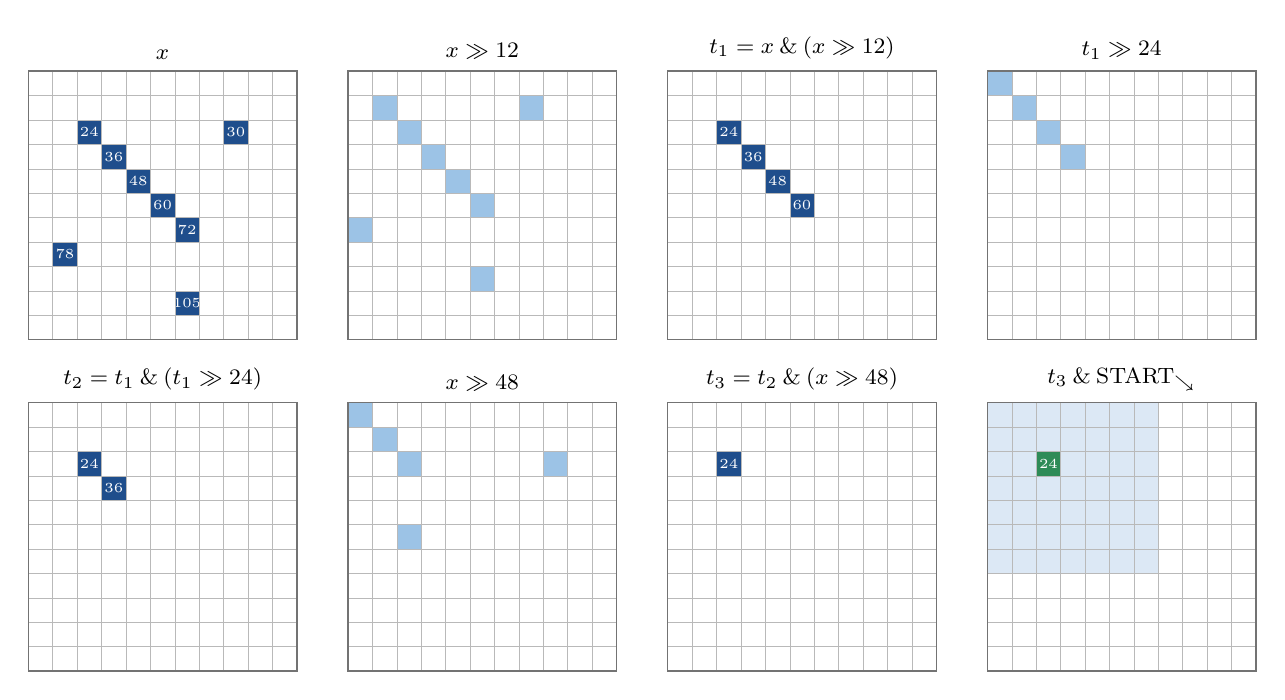
\begin{tikzpicture}
\begin{scope}[shift={(0.000,0.000)}]
\fill[bbX] (0.620,-0.620) rectangle ++(0.310,-0.310);
\node[text=white,inner sep=0,font=\fontsize{5}{5}\selectfont] at (0.775,-0.775) {24};
\fill[bbX] (2.480,-0.620) rectangle ++(0.310,-0.310);
\node[text=white,inner sep=0,font=\fontsize{5}{5}\selectfont] at (2.635,-0.775) {30};
\fill[bbX] (0.930,-0.930) rectangle ++(0.310,-0.310);
\node[text=white,inner sep=0,font=\fontsize{5}{5}\selectfont] at (1.085,-1.085) {36};
\fill[bbX] (1.240,-1.240) rectangle ++(0.310,-0.310);
\node[text=white,inner sep=0,font=\fontsize{5}{5}\selectfont] at (1.395,-1.395) {48};
\fill[bbX] (1.550,-1.550) rectangle ++(0.310,-0.310);
\node[text=white,inner sep=0,font=\fontsize{5}{5}\selectfont] at (1.705,-1.705) {60};
\fill[bbX] (1.860,-1.860) rectangle ++(0.310,-0.310);
\node[text=white,inner sep=0,font=\fontsize{5}{5}\selectfont] at (2.015,-2.015) {72};
\fill[bbX] (0.310,-2.170) rectangle ++(0.310,-0.310);
\node[text=white,inner sep=0,font=\fontsize{5}{5}\selectfont] at (0.465,-2.325) {78};
\fill[bbX] (1.860,-2.790) rectangle ++(0.310,-0.310);
\node[text=white,inner sep=0,font=\fontsize{5}{5}\selectfont] at (2.015,-2.945) {105};
\draw[gray!55,line width=.2pt] (0,0) grid[step=0.310] (3.410,-3.410);
\draw[gray!90!black,line width=.5pt] (0,0) rectangle (3.410,-3.410);
\node[anchor=south,font=\footnotesize] at (1.705,0.03) {$x$};
\end{scope}
\begin{scope}[shift={(4.060,0.000)}]
\fill[bbNhat] (0.310,-0.310) rectangle ++(0.310,-0.310);
\fill[bbNhat] (2.170,-0.310) rectangle ++(0.310,-0.310);
\fill[bbNhat] (0.620,-0.620) rectangle ++(0.310,-0.310);
\fill[bbNhat] (0.930,-0.930) rectangle ++(0.310,-0.310);
\fill[bbNhat] (1.240,-1.240) rectangle ++(0.310,-0.310);
\fill[bbNhat] (1.550,-1.550) rectangle ++(0.310,-0.310);
\fill[bbNhat] (0.000,-1.860) rectangle ++(0.310,-0.310);
\fill[bbNhat] (1.550,-2.480) rectangle ++(0.310,-0.310);
\draw[gray!55,line width=.2pt] (0,0) grid[step=0.310] (3.410,-3.410);
\draw[gray!90!black,line width=.5pt] (0,0) rectangle (3.410,-3.410);
\node[anchor=south,font=\footnotesize] at (1.705,0.03) {$x \gg 12$};
\end{scope}
\begin{scope}[shift={(8.120,0.000)}]
\fill[bbX] (0.620,-0.620) rectangle ++(0.310,-0.310);
\node[text=white,inner sep=0,font=\fontsize{5}{5}\selectfont] at (0.775,-0.775) {24};
\fill[bbX] (0.930,-0.930) rectangle ++(0.310,-0.310);
\node[text=white,inner sep=0,font=\fontsize{5}{5}\selectfont] at (1.085,-1.085) {36};
\fill[bbX] (1.240,-1.240) rectangle ++(0.310,-0.310);
\node[text=white,inner sep=0,font=\fontsize{5}{5}\selectfont] at (1.395,-1.395) {48};
\fill[bbX] (1.550,-1.550) rectangle ++(0.310,-0.310);
\node[text=white,inner sep=0,font=\fontsize{5}{5}\selectfont] at (1.705,-1.705) {60};
\draw[gray!55,line width=.2pt] (0,0) grid[step=0.310] (3.410,-3.410);
\draw[gray!90!black,line width=.5pt] (0,0) rectangle (3.410,-3.410);
\node[anchor=south,font=\footnotesize] at (1.705,0.03) {$t_1 = x \mathbin{\&} (x \gg 12)$};
\end{scope}
\begin{scope}[shift={(12.180,0.000)}]
\fill[bbNhat] (0.000,0.000) rectangle ++(0.310,-0.310);
\fill[bbNhat] (0.310,-0.310) rectangle ++(0.310,-0.310);
\fill[bbNhat] (0.620,-0.620) rectangle ++(0.310,-0.310);
\fill[bbNhat] (0.930,-0.930) rectangle ++(0.310,-0.310);
\draw[gray!55,line width=.2pt] (0,0) grid[step=0.310] (3.410,-3.410);
\draw[gray!90!black,line width=.5pt] (0,0) rectangle (3.410,-3.410);
\node[anchor=south,font=\footnotesize] at (1.705,0.03) {$t_1 \gg 24$};
\end{scope}
\begin{scope}[shift={(0.000,-4.210)}]
\fill[bbX] (0.620,-0.620) rectangle ++(0.310,-0.310);
\node[text=white,inner sep=0,font=\fontsize{5}{5}\selectfont] at (0.775,-0.775) {24};
\fill[bbX] (0.930,-0.930) rectangle ++(0.310,-0.310);
\node[text=white,inner sep=0,font=\fontsize{5}{5}\selectfont] at (1.085,-1.085) {36};
\draw[gray!55,line width=.2pt] (0,0) grid[step=0.310] (3.410,-3.410);
\draw[gray!90!black,line width=.5pt] (0,0) rectangle (3.410,-3.410);
\node[anchor=south,font=\footnotesize] at (1.705,0.03) {$t_2 = t_1 \mathbin{\&} (t_1 \gg 24)$};
\end{scope}
\begin{scope}[shift={(4.060,-4.210)}]
\fill[bbNhat] (0.000,0.000) rectangle ++(0.310,-0.310);
\fill[bbNhat] (0.310,-0.310) rectangle ++(0.310,-0.310);
\fill[bbNhat] (0.620,-0.620) rectangle ++(0.310,-0.310);
\fill[bbNhat] (2.480,-0.620) rectangle ++(0.310,-0.310);
\fill[bbNhat] (0.620,-1.550) rectangle ++(0.310,-0.310);
\draw[gray!55,line width=.2pt] (0,0) grid[step=0.310] (3.410,-3.410);
\draw[gray!90!black,line width=.5pt] (0,0) rectangle (3.410,-3.410);
\node[anchor=south,font=\footnotesize] at (1.705,0.03) {$x \gg 48$};
\end{scope}
\begin{scope}[shift={(8.120,-4.210)}]
\fill[bbX] (0.620,-0.620) rectangle ++(0.310,-0.310);
\node[text=white,inner sep=0,font=\fontsize{5}{5}\selectfont] at (0.775,-0.775) {24};
\draw[gray!55,line width=.2pt] (0,0) grid[step=0.310] (3.410,-3.410);
\draw[gray!90!black,line width=.5pt] (0,0) rectangle (3.410,-3.410);
\node[anchor=south,font=\footnotesize] at (1.705,0.03) {$t_3 = t_2 \mathbin{\&} (x \gg 48)$};
\end{scope}
\begin{scope}[shift={(12.180,-4.210)}]
\fill[bbMat] (0.000,0.000) rectangle ++(0.310,-0.310);
\fill[bbMat] (0.310,0.000) rectangle ++(0.310,-0.310);
\fill[bbMat] (0.620,0.000) rectangle ++(0.310,-0.310);
\fill[bbMat] (0.930,0.000) rectangle ++(0.310,-0.310);
\fill[bbMat] (1.240,0.000) rectangle ++(0.310,-0.310);
\fill[bbMat] (1.550,0.000) rectangle ++(0.310,-0.310);
\fill[bbMat] (1.860,0.000) rectangle ++(0.310,-0.310);
\fill[bbMat] (0.000,-0.310) rectangle ++(0.310,-0.310);
\fill[bbMat] (0.310,-0.310) rectangle ++(0.310,-0.310);
\fill[bbMat] (0.620,-0.310) rectangle ++(0.310,-0.310);
\fill[bbMat] (0.930,-0.310) rectangle ++(0.310,-0.310);
\fill[bbMat] (1.240,-0.310) rectangle ++(0.310,-0.310);
\fill[bbMat] (1.550,-0.310) rectangle ++(0.310,-0.310);
\fill[bbMat] (1.860,-0.310) rectangle ++(0.310,-0.310);
\fill[bbMat] (0.000,-0.620) rectangle ++(0.310,-0.310);
\fill[bbMat] (0.310,-0.620) rectangle ++(0.310,-0.310);
\fill[bbKq] (0.620,-0.620) rectangle ++(0.310,-0.310);
\node[text=white,inner sep=0,font=\fontsize{5}{5}\selectfont] at (0.775,-0.775) {24};
\fill[bbMat] (0.930,-0.620) rectangle ++(0.310,-0.310);
\fill[bbMat] (1.240,-0.620) rectangle ++(0.310,-0.310);
\fill[bbMat] (1.550,-0.620) rectangle ++(0.310,-0.310);
\fill[bbMat] (1.860,-0.620) rectangle ++(0.310,-0.310);
\fill[bbMat] (0.000,-0.930) rectangle ++(0.310,-0.310);
\fill[bbMat] (0.310,-0.930) rectangle ++(0.310,-0.310);
\fill[bbMat] (0.620,-0.930) rectangle ++(0.310,-0.310);
\fill[bbMat] (0.930,-0.930) rectangle ++(0.310,-0.310);
\fill[bbMat] (1.240,-0.930) rectangle ++(0.310,-0.310);
\fill[bbMat] (1.550,-0.930) rectangle ++(0.310,-0.310);
\fill[bbMat] (1.860,-0.930) rectangle ++(0.310,-0.310);
\fill[bbMat] (0.000,-1.240) rectangle ++(0.310,-0.310);
\fill[bbMat] (0.310,-1.240) rectangle ++(0.310,-0.310);
\fill[bbMat] (0.620,-1.240) rectangle ++(0.310,-0.310);
\fill[bbMat] (0.930,-1.240) rectangle ++(0.310,-0.310);
\fill[bbMat] (1.240,-1.240) rectangle ++(0.310,-0.310);
\fill[bbMat] (1.550,-1.240) rectangle ++(0.310,-0.310);
\fill[bbMat] (1.860,-1.240) rectangle ++(0.310,-0.310);
\fill[bbMat] (0.000,-1.550) rectangle ++(0.310,-0.310);
\fill[bbMat] (0.310,-1.550) rectangle ++(0.310,-0.310);
\fill[bbMat] (0.620,-1.550) rectangle ++(0.310,-0.310);
\fill[bbMat] (0.930,-1.550) rectangle ++(0.310,-0.310);
\fill[bbMat] (1.240,-1.550) rectangle ++(0.310,-0.310);
\fill[bbMat] (1.550,-1.550) rectangle ++(0.310,-0.310);
\fill[bbMat] (1.860,-1.550) rectangle ++(0.310,-0.310);
\fill[bbMat] (0.000,-1.860) rectangle ++(0.310,-0.310);
\fill[bbMat] (0.310,-1.860) rectangle ++(0.310,-0.310);
\fill[bbMat] (0.620,-1.860) rectangle ++(0.310,-0.310);
\fill[bbMat] (0.930,-1.860) rectangle ++(0.310,-0.310);
\fill[bbMat] (1.240,-1.860) rectangle ++(0.310,-0.310);
\fill[bbMat] (1.550,-1.860) rectangle ++(0.310,-0.310);
\fill[bbMat] (1.860,-1.860) rectangle ++(0.310,-0.310);
\draw[gray!55,line width=.2pt] (0,0) grid[step=0.310] (3.410,-3.410);
\draw[gray!90!black,line width=.5pt] (0,0) rectangle (3.410,-3.410);
\node[anchor=south,font=\footnotesize] at (1.705,0.03) {$t_3 \mathbin{\&} \mathrm{START}_{\searrow}$};
\end{scope}
\end{tikzpicture}

  \caption{Các bước của \texttt{has\_five} với $d = 12$. Ô xanh nhạt là kết quả phép dịch, ô xanh đậm là kết quả phép AND, số trong ô là chỉ số bit. Ô xanh lá là bit 24 còn lại sau khi lọc qua mặt nạ.}
  \label{fig:has-five}
\end{figure}

Luật ``từ 5 quân trở lên'' được xử lý tự nhiên: dãy 6 quân cho $t_3$ có hai bit, vẫn khác 0. Quân chặn hai đầu không tham gia vào phép tính nên dãy bị chặn vẫn thắng, đúng với luật của đề tài. Chi phí là 3 phép dịch và 4 phép AND cho mỗi hướng, tối đa 12 phép dịch cho cả bàn, không phụ thuộc số quân.

\begin{vidu}[Dãy 5 giả do lọt hàng]
Năm quân $(2,8)$, $(2,9)$, $(2,10)$, $(3,0)$, $(3,1)$ có các bit 30--34 liên tiếp nên với $d = 1$ ba bước trên vẫn cho $t_3 = \{30\}$. Nhưng bit 30 là ô $(2, 8)$, có $c = 8 > 6$, không thuộc $\mathrm{START}_{\text{ngang}}$, nên kết quả bị loại. Trường hợp chéo cũng tương tự: các bit $8, 20, 32, 44, 56$ cách đều 12 cho $t_3 = \{8\}$, là ô $(0, 8)$ có $c = 8 > 6$, cũng bị loại (Hình~\ref{fig:lot-hang}).
\end{vidu}

\begin{figure}[H]
  \centering
  % Sinh tự động bởi report/scripts/ve_hinh_bitboard.py, đừng sửa tay.
\definecolor{bbX}{HTML}{1F4E8C}
\definecolor{bbO}{HTML}{C8553D}
\definecolor{bbKq}{HTML}{2E8B57}
\definecolor{bbSai}{HTML}{D7263D}
\definecolor{bbMat}{HTML}{DCE8F5}
\definecolor{bbVang}{HTML}{FBE7A1}
\definecolor{bbXam}{HTML}{BDBDBD}
\definecolor{bbNhat}{HTML}{9CC3E6}
\begin{tikzpicture}
\begin{scope}[shift={(0.000,0.000)}]
\fill[bbX] (2.480,-0.620) rectangle ++(0.310,-0.310);
\node[text=white,inner sep=0,font=\fontsize{5}{5}\selectfont] at (2.635,-0.775) {30};
\fill[bbX] (2.790,-0.620) rectangle ++(0.310,-0.310);
\node[text=white,inner sep=0,font=\fontsize{5}{5}\selectfont] at (2.945,-0.775) {31};
\fill[bbX] (3.100,-0.620) rectangle ++(0.310,-0.310);
\node[text=white,inner sep=0,font=\fontsize{5}{5}\selectfont] at (3.255,-0.775) {32};
\fill[bbX] (0.000,-0.930) rectangle ++(0.310,-0.310);
\node[text=white,inner sep=0,font=\fontsize{5}{5}\selectfont] at (0.155,-1.085) {33};
\fill[bbX] (0.310,-0.930) rectangle ++(0.310,-0.310);
\node[text=white,inner sep=0,font=\fontsize{5}{5}\selectfont] at (0.465,-1.085) {34};
\draw[gray!55,line width=.2pt] (0,0) grid[step=0.310] (3.410,-3.410);
\draw[gray!90!black,line width=.5pt] (0,0) rectangle (3.410,-3.410);
\node[anchor=south,font=\footnotesize] at (1.705,0.03) {$x$ (bước $d=1$)};
\end{scope}
\begin{scope}[shift={(4.060,0.000)}]
\fill[bbSai] (2.480,-0.620) rectangle ++(0.310,-0.310);
\node[text=white,inner sep=0,font=\fontsize{5}{5}\selectfont] at (2.635,-0.775) {30};
\draw[gray!55,line width=.2pt] (0,0) grid[step=0.310] (3.410,-3.410);
\draw[gray!90!black,line width=.5pt] (0,0) rectangle (3.410,-3.410);
\node[anchor=south,font=\footnotesize] at (1.705,0.03) {$t_3$ (dãy 5 giả)};
\end{scope}
\begin{scope}[shift={(8.120,0.000)}]
\fill[bbMat] (0.000,0.000) rectangle ++(0.310,-0.310);
\fill[bbMat] (0.310,0.000) rectangle ++(0.310,-0.310);
\fill[bbMat] (0.620,0.000) rectangle ++(0.310,-0.310);
\fill[bbMat] (0.930,0.000) rectangle ++(0.310,-0.310);
\fill[bbMat] (1.240,0.000) rectangle ++(0.310,-0.310);
\fill[bbMat] (1.550,0.000) rectangle ++(0.310,-0.310);
\fill[bbMat] (1.860,0.000) rectangle ++(0.310,-0.310);
\fill[bbMat] (0.000,-0.310) rectangle ++(0.310,-0.310);
\fill[bbMat] (0.310,-0.310) rectangle ++(0.310,-0.310);
\fill[bbMat] (0.620,-0.310) rectangle ++(0.310,-0.310);
\fill[bbMat] (0.930,-0.310) rectangle ++(0.310,-0.310);
\fill[bbMat] (1.240,-0.310) rectangle ++(0.310,-0.310);
\fill[bbMat] (1.550,-0.310) rectangle ++(0.310,-0.310);
\fill[bbMat] (1.860,-0.310) rectangle ++(0.310,-0.310);
\fill[bbMat] (0.000,-0.620) rectangle ++(0.310,-0.310);
\fill[bbMat] (0.310,-0.620) rectangle ++(0.310,-0.310);
\fill[bbMat] (0.620,-0.620) rectangle ++(0.310,-0.310);
\fill[bbMat] (0.930,-0.620) rectangle ++(0.310,-0.310);
\fill[bbMat] (1.240,-0.620) rectangle ++(0.310,-0.310);
\fill[bbMat] (1.550,-0.620) rectangle ++(0.310,-0.310);
\fill[bbMat] (1.860,-0.620) rectangle ++(0.310,-0.310);
\fill[bbMat] (0.000,-0.930) rectangle ++(0.310,-0.310);
\fill[bbMat] (0.310,-0.930) rectangle ++(0.310,-0.310);
\fill[bbMat] (0.620,-0.930) rectangle ++(0.310,-0.310);
\fill[bbMat] (0.930,-0.930) rectangle ++(0.310,-0.310);
\fill[bbMat] (1.240,-0.930) rectangle ++(0.310,-0.310);
\fill[bbMat] (1.550,-0.930) rectangle ++(0.310,-0.310);
\fill[bbMat] (1.860,-0.930) rectangle ++(0.310,-0.310);
\fill[bbMat] (0.000,-1.240) rectangle ++(0.310,-0.310);
\fill[bbMat] (0.310,-1.240) rectangle ++(0.310,-0.310);
\fill[bbMat] (0.620,-1.240) rectangle ++(0.310,-0.310);
\fill[bbMat] (0.930,-1.240) rectangle ++(0.310,-0.310);
\fill[bbMat] (1.240,-1.240) rectangle ++(0.310,-0.310);
\fill[bbMat] (1.550,-1.240) rectangle ++(0.310,-0.310);
\fill[bbMat] (1.860,-1.240) rectangle ++(0.310,-0.310);
\fill[bbMat] (0.000,-1.550) rectangle ++(0.310,-0.310);
\fill[bbMat] (0.310,-1.550) rectangle ++(0.310,-0.310);
\fill[bbMat] (0.620,-1.550) rectangle ++(0.310,-0.310);
\fill[bbMat] (0.930,-1.550) rectangle ++(0.310,-0.310);
\fill[bbMat] (1.240,-1.550) rectangle ++(0.310,-0.310);
\fill[bbMat] (1.550,-1.550) rectangle ++(0.310,-0.310);
\fill[bbMat] (1.860,-1.550) rectangle ++(0.310,-0.310);
\fill[bbMat] (0.000,-1.860) rectangle ++(0.310,-0.310);
\fill[bbMat] (0.310,-1.860) rectangle ++(0.310,-0.310);
\fill[bbMat] (0.620,-1.860) rectangle ++(0.310,-0.310);
\fill[bbMat] (0.930,-1.860) rectangle ++(0.310,-0.310);
\fill[bbMat] (1.240,-1.860) rectangle ++(0.310,-0.310);
\fill[bbMat] (1.550,-1.860) rectangle ++(0.310,-0.310);
\fill[bbMat] (1.860,-1.860) rectangle ++(0.310,-0.310);
\fill[bbMat] (0.000,-2.170) rectangle ++(0.310,-0.310);
\fill[bbMat] (0.310,-2.170) rectangle ++(0.310,-0.310);
\fill[bbMat] (0.620,-2.170) rectangle ++(0.310,-0.310);
\fill[bbMat] (0.930,-2.170) rectangle ++(0.310,-0.310);
\fill[bbMat] (1.240,-2.170) rectangle ++(0.310,-0.310);
\fill[bbMat] (1.550,-2.170) rectangle ++(0.310,-0.310);
\fill[bbMat] (1.860,-2.170) rectangle ++(0.310,-0.310);
\fill[bbMat] (0.000,-2.480) rectangle ++(0.310,-0.310);
\fill[bbMat] (0.310,-2.480) rectangle ++(0.310,-0.310);
\fill[bbMat] (0.620,-2.480) rectangle ++(0.310,-0.310);
\fill[bbMat] (0.930,-2.480) rectangle ++(0.310,-0.310);
\fill[bbMat] (1.240,-2.480) rectangle ++(0.310,-0.310);
\fill[bbMat] (1.550,-2.480) rectangle ++(0.310,-0.310);
\fill[bbMat] (1.860,-2.480) rectangle ++(0.310,-0.310);
\fill[bbMat] (0.000,-2.790) rectangle ++(0.310,-0.310);
\fill[bbMat] (0.310,-2.790) rectangle ++(0.310,-0.310);
\fill[bbMat] (0.620,-2.790) rectangle ++(0.310,-0.310);
\fill[bbMat] (0.930,-2.790) rectangle ++(0.310,-0.310);
\fill[bbMat] (1.240,-2.790) rectangle ++(0.310,-0.310);
\fill[bbMat] (1.550,-2.790) rectangle ++(0.310,-0.310);
\fill[bbMat] (1.860,-2.790) rectangle ++(0.310,-0.310);
\fill[bbMat] (0.000,-3.100) rectangle ++(0.310,-0.310);
\fill[bbMat] (0.310,-3.100) rectangle ++(0.310,-0.310);
\fill[bbMat] (0.620,-3.100) rectangle ++(0.310,-0.310);
\fill[bbMat] (0.930,-3.100) rectangle ++(0.310,-0.310);
\fill[bbMat] (1.240,-3.100) rectangle ++(0.310,-0.310);
\fill[bbMat] (1.550,-3.100) rectangle ++(0.310,-0.310);
\fill[bbMat] (1.860,-3.100) rectangle ++(0.310,-0.310);
\draw[gray!55,line width=.2pt] (0,0) grid[step=0.310] (3.410,-3.410);
\draw[gray!90!black,line width=.5pt] (0,0) rectangle (3.410,-3.410);
\node[anchor=south,font=\footnotesize] at (1.705,0.03) {$\mathrm{START}_{\text{ngang}}$};
\end{scope}
\begin{scope}[shift={(12.180,0.000)}]
\fill[bbMat] (0.000,0.000) rectangle ++(0.310,-0.310);
\fill[bbMat] (0.310,0.000) rectangle ++(0.310,-0.310);
\fill[bbMat] (0.620,0.000) rectangle ++(0.310,-0.310);
\fill[bbMat] (0.930,0.000) rectangle ++(0.310,-0.310);
\fill[bbMat] (1.240,0.000) rectangle ++(0.310,-0.310);
\fill[bbMat] (1.550,0.000) rectangle ++(0.310,-0.310);
\fill[bbMat] (1.860,0.000) rectangle ++(0.310,-0.310);
\fill[bbMat] (0.000,-0.310) rectangle ++(0.310,-0.310);
\fill[bbMat] (0.310,-0.310) rectangle ++(0.310,-0.310);
\fill[bbMat] (0.620,-0.310) rectangle ++(0.310,-0.310);
\fill[bbMat] (0.930,-0.310) rectangle ++(0.310,-0.310);
\fill[bbMat] (1.240,-0.310) rectangle ++(0.310,-0.310);
\fill[bbMat] (1.550,-0.310) rectangle ++(0.310,-0.310);
\fill[bbMat] (1.860,-0.310) rectangle ++(0.310,-0.310);
\fill[bbMat] (0.000,-0.620) rectangle ++(0.310,-0.310);
\fill[bbMat] (0.310,-0.620) rectangle ++(0.310,-0.310);
\fill[bbMat] (0.620,-0.620) rectangle ++(0.310,-0.310);
\fill[bbMat] (0.930,-0.620) rectangle ++(0.310,-0.310);
\fill[bbMat] (1.240,-0.620) rectangle ++(0.310,-0.310);
\fill[bbMat] (1.550,-0.620) rectangle ++(0.310,-0.310);
\fill[bbMat] (1.860,-0.620) rectangle ++(0.310,-0.310);
\fill[bbMat] (0.000,-0.930) rectangle ++(0.310,-0.310);
\fill[bbMat] (0.310,-0.930) rectangle ++(0.310,-0.310);
\fill[bbMat] (0.620,-0.930) rectangle ++(0.310,-0.310);
\fill[bbMat] (0.930,-0.930) rectangle ++(0.310,-0.310);
\fill[bbMat] (1.240,-0.930) rectangle ++(0.310,-0.310);
\fill[bbMat] (1.550,-0.930) rectangle ++(0.310,-0.310);
\fill[bbMat] (1.860,-0.930) rectangle ++(0.310,-0.310);
\fill[bbMat] (0.000,-1.240) rectangle ++(0.310,-0.310);
\fill[bbMat] (0.310,-1.240) rectangle ++(0.310,-0.310);
\fill[bbMat] (0.620,-1.240) rectangle ++(0.310,-0.310);
\fill[bbMat] (0.930,-1.240) rectangle ++(0.310,-0.310);
\fill[bbMat] (1.240,-1.240) rectangle ++(0.310,-0.310);
\fill[bbMat] (1.550,-1.240) rectangle ++(0.310,-0.310);
\fill[bbMat] (1.860,-1.240) rectangle ++(0.310,-0.310);
\fill[bbMat] (0.000,-1.550) rectangle ++(0.310,-0.310);
\fill[bbMat] (0.310,-1.550) rectangle ++(0.310,-0.310);
\fill[bbMat] (0.620,-1.550) rectangle ++(0.310,-0.310);
\fill[bbMat] (0.930,-1.550) rectangle ++(0.310,-0.310);
\fill[bbMat] (1.240,-1.550) rectangle ++(0.310,-0.310);
\fill[bbMat] (1.550,-1.550) rectangle ++(0.310,-0.310);
\fill[bbMat] (1.860,-1.550) rectangle ++(0.310,-0.310);
\fill[bbMat] (0.000,-1.860) rectangle ++(0.310,-0.310);
\fill[bbMat] (0.310,-1.860) rectangle ++(0.310,-0.310);
\fill[bbMat] (0.620,-1.860) rectangle ++(0.310,-0.310);
\fill[bbMat] (0.930,-1.860) rectangle ++(0.310,-0.310);
\fill[bbMat] (1.240,-1.860) rectangle ++(0.310,-0.310);
\fill[bbMat] (1.550,-1.860) rectangle ++(0.310,-0.310);
\fill[bbMat] (1.860,-1.860) rectangle ++(0.310,-0.310);
\fill[bbMat] (0.000,-2.170) rectangle ++(0.310,-0.310);
\fill[bbMat] (0.310,-2.170) rectangle ++(0.310,-0.310);
\fill[bbMat] (0.620,-2.170) rectangle ++(0.310,-0.310);
\fill[bbMat] (0.930,-2.170) rectangle ++(0.310,-0.310);
\fill[bbMat] (1.240,-2.170) rectangle ++(0.310,-0.310);
\fill[bbMat] (1.550,-2.170) rectangle ++(0.310,-0.310);
\fill[bbMat] (1.860,-2.170) rectangle ++(0.310,-0.310);
\fill[bbMat] (0.000,-2.480) rectangle ++(0.310,-0.310);
\fill[bbMat] (0.310,-2.480) rectangle ++(0.310,-0.310);
\fill[bbMat] (0.620,-2.480) rectangle ++(0.310,-0.310);
\fill[bbMat] (0.930,-2.480) rectangle ++(0.310,-0.310);
\fill[bbMat] (1.240,-2.480) rectangle ++(0.310,-0.310);
\fill[bbMat] (1.550,-2.480) rectangle ++(0.310,-0.310);
\fill[bbMat] (1.860,-2.480) rectangle ++(0.310,-0.310);
\fill[bbMat] (0.000,-2.790) rectangle ++(0.310,-0.310);
\fill[bbMat] (0.310,-2.790) rectangle ++(0.310,-0.310);
\fill[bbMat] (0.620,-2.790) rectangle ++(0.310,-0.310);
\fill[bbMat] (0.930,-2.790) rectangle ++(0.310,-0.310);
\fill[bbMat] (1.240,-2.790) rectangle ++(0.310,-0.310);
\fill[bbMat] (1.550,-2.790) rectangle ++(0.310,-0.310);
\fill[bbMat] (1.860,-2.790) rectangle ++(0.310,-0.310);
\fill[bbMat] (0.000,-3.100) rectangle ++(0.310,-0.310);
\fill[bbMat] (0.310,-3.100) rectangle ++(0.310,-0.310);
\fill[bbMat] (0.620,-3.100) rectangle ++(0.310,-0.310);
\fill[bbMat] (0.930,-3.100) rectangle ++(0.310,-0.310);
\fill[bbMat] (1.240,-3.100) rectangle ++(0.310,-0.310);
\fill[bbMat] (1.550,-3.100) rectangle ++(0.310,-0.310);
\fill[bbMat] (1.860,-3.100) rectangle ++(0.310,-0.310);
\draw[gray!55,line width=.2pt] (0,0) grid[step=0.310] (3.410,-3.410);
\draw[gray!90!black,line width=.5pt] (0,0) rectangle (3.410,-3.410);
\node[anchor=south,font=\footnotesize] at (1.705,0.03) {$t_3 \mathbin{\&} \mathrm{START} = 0$};
\end{scope}
\begin{scope}[shift={(0.000,-4.210)}]
\fill[bbX] (2.480,0.000) rectangle ++(0.310,-0.310);
\node[text=white,inner sep=0,font=\fontsize{5}{5}\selectfont] at (2.635,-0.155) {8};
\fill[bbX] (2.790,-0.310) rectangle ++(0.310,-0.310);
\node[text=white,inner sep=0,font=\fontsize{5}{5}\selectfont] at (2.945,-0.465) {20};
\fill[bbX] (3.100,-0.620) rectangle ++(0.310,-0.310);
\node[text=white,inner sep=0,font=\fontsize{5}{5}\selectfont] at (3.255,-0.775) {32};
\fill[bbX] (0.000,-1.240) rectangle ++(0.310,-0.310);
\node[text=white,inner sep=0,font=\fontsize{5}{5}\selectfont] at (0.155,-1.395) {44};
\fill[bbX] (0.310,-1.550) rectangle ++(0.310,-0.310);
\node[text=white,inner sep=0,font=\fontsize{5}{5}\selectfont] at (0.465,-1.705) {56};
\draw[gray!55,line width=.2pt] (0,0) grid[step=0.310] (3.410,-3.410);
\draw[gray!90!black,line width=.5pt] (0,0) rectangle (3.410,-3.410);
\node[anchor=south,font=\footnotesize] at (1.705,0.03) {$x$ (bước $d=12$)};
\end{scope}
\begin{scope}[shift={(4.060,-4.210)}]
\fill[bbSai] (2.480,0.000) rectangle ++(0.310,-0.310);
\node[text=white,inner sep=0,font=\fontsize{5}{5}\selectfont] at (2.635,-0.155) {8};
\draw[gray!55,line width=.2pt] (0,0) grid[step=0.310] (3.410,-3.410);
\draw[gray!90!black,line width=.5pt] (0,0) rectangle (3.410,-3.410);
\node[anchor=south,font=\footnotesize] at (1.705,0.03) {$t_3$ (dãy 5 giả)};
\end{scope}
\begin{scope}[shift={(8.120,-4.210)}]
\fill[bbMat] (0.000,0.000) rectangle ++(0.310,-0.310);
\fill[bbMat] (0.310,0.000) rectangle ++(0.310,-0.310);
\fill[bbMat] (0.620,0.000) rectangle ++(0.310,-0.310);
\fill[bbMat] (0.930,0.000) rectangle ++(0.310,-0.310);
\fill[bbMat] (1.240,0.000) rectangle ++(0.310,-0.310);
\fill[bbMat] (1.550,0.000) rectangle ++(0.310,-0.310);
\fill[bbMat] (1.860,0.000) rectangle ++(0.310,-0.310);
\fill[bbMat] (0.000,-0.310) rectangle ++(0.310,-0.310);
\fill[bbMat] (0.310,-0.310) rectangle ++(0.310,-0.310);
\fill[bbMat] (0.620,-0.310) rectangle ++(0.310,-0.310);
\fill[bbMat] (0.930,-0.310) rectangle ++(0.310,-0.310);
\fill[bbMat] (1.240,-0.310) rectangle ++(0.310,-0.310);
\fill[bbMat] (1.550,-0.310) rectangle ++(0.310,-0.310);
\fill[bbMat] (1.860,-0.310) rectangle ++(0.310,-0.310);
\fill[bbMat] (0.000,-0.620) rectangle ++(0.310,-0.310);
\fill[bbMat] (0.310,-0.620) rectangle ++(0.310,-0.310);
\fill[bbMat] (0.620,-0.620) rectangle ++(0.310,-0.310);
\fill[bbMat] (0.930,-0.620) rectangle ++(0.310,-0.310);
\fill[bbMat] (1.240,-0.620) rectangle ++(0.310,-0.310);
\fill[bbMat] (1.550,-0.620) rectangle ++(0.310,-0.310);
\fill[bbMat] (1.860,-0.620) rectangle ++(0.310,-0.310);
\fill[bbMat] (0.000,-0.930) rectangle ++(0.310,-0.310);
\fill[bbMat] (0.310,-0.930) rectangle ++(0.310,-0.310);
\fill[bbMat] (0.620,-0.930) rectangle ++(0.310,-0.310);
\fill[bbMat] (0.930,-0.930) rectangle ++(0.310,-0.310);
\fill[bbMat] (1.240,-0.930) rectangle ++(0.310,-0.310);
\fill[bbMat] (1.550,-0.930) rectangle ++(0.310,-0.310);
\fill[bbMat] (1.860,-0.930) rectangle ++(0.310,-0.310);
\fill[bbMat] (0.000,-1.240) rectangle ++(0.310,-0.310);
\fill[bbMat] (0.310,-1.240) rectangle ++(0.310,-0.310);
\fill[bbMat] (0.620,-1.240) rectangle ++(0.310,-0.310);
\fill[bbMat] (0.930,-1.240) rectangle ++(0.310,-0.310);
\fill[bbMat] (1.240,-1.240) rectangle ++(0.310,-0.310);
\fill[bbMat] (1.550,-1.240) rectangle ++(0.310,-0.310);
\fill[bbMat] (1.860,-1.240) rectangle ++(0.310,-0.310);
\fill[bbMat] (0.000,-1.550) rectangle ++(0.310,-0.310);
\fill[bbMat] (0.310,-1.550) rectangle ++(0.310,-0.310);
\fill[bbMat] (0.620,-1.550) rectangle ++(0.310,-0.310);
\fill[bbMat] (0.930,-1.550) rectangle ++(0.310,-0.310);
\fill[bbMat] (1.240,-1.550) rectangle ++(0.310,-0.310);
\fill[bbMat] (1.550,-1.550) rectangle ++(0.310,-0.310);
\fill[bbMat] (1.860,-1.550) rectangle ++(0.310,-0.310);
\fill[bbMat] (0.000,-1.860) rectangle ++(0.310,-0.310);
\fill[bbMat] (0.310,-1.860) rectangle ++(0.310,-0.310);
\fill[bbMat] (0.620,-1.860) rectangle ++(0.310,-0.310);
\fill[bbMat] (0.930,-1.860) rectangle ++(0.310,-0.310);
\fill[bbMat] (1.240,-1.860) rectangle ++(0.310,-0.310);
\fill[bbMat] (1.550,-1.860) rectangle ++(0.310,-0.310);
\fill[bbMat] (1.860,-1.860) rectangle ++(0.310,-0.310);
\draw[gray!55,line width=.2pt] (0,0) grid[step=0.310] (3.410,-3.410);
\draw[gray!90!black,line width=.5pt] (0,0) rectangle (3.410,-3.410);
\node[anchor=south,font=\footnotesize] at (1.705,0.03) {$\mathrm{START}_{\searrow}$};
\end{scope}
\begin{scope}[shift={(12.180,-4.210)}]
\fill[bbMat] (0.000,0.000) rectangle ++(0.310,-0.310);
\fill[bbMat] (0.310,0.000) rectangle ++(0.310,-0.310);
\fill[bbMat] (0.620,0.000) rectangle ++(0.310,-0.310);
\fill[bbMat] (0.930,0.000) rectangle ++(0.310,-0.310);
\fill[bbMat] (1.240,0.000) rectangle ++(0.310,-0.310);
\fill[bbMat] (1.550,0.000) rectangle ++(0.310,-0.310);
\fill[bbMat] (1.860,0.000) rectangle ++(0.310,-0.310);
\fill[bbMat] (0.000,-0.310) rectangle ++(0.310,-0.310);
\fill[bbMat] (0.310,-0.310) rectangle ++(0.310,-0.310);
\fill[bbMat] (0.620,-0.310) rectangle ++(0.310,-0.310);
\fill[bbMat] (0.930,-0.310) rectangle ++(0.310,-0.310);
\fill[bbMat] (1.240,-0.310) rectangle ++(0.310,-0.310);
\fill[bbMat] (1.550,-0.310) rectangle ++(0.310,-0.310);
\fill[bbMat] (1.860,-0.310) rectangle ++(0.310,-0.310);
\fill[bbMat] (0.000,-0.620) rectangle ++(0.310,-0.310);
\fill[bbMat] (0.310,-0.620) rectangle ++(0.310,-0.310);
\fill[bbMat] (0.620,-0.620) rectangle ++(0.310,-0.310);
\fill[bbMat] (0.930,-0.620) rectangle ++(0.310,-0.310);
\fill[bbMat] (1.240,-0.620) rectangle ++(0.310,-0.310);
\fill[bbMat] (1.550,-0.620) rectangle ++(0.310,-0.310);
\fill[bbMat] (1.860,-0.620) rectangle ++(0.310,-0.310);
\fill[bbMat] (0.000,-0.930) rectangle ++(0.310,-0.310);
\fill[bbMat] (0.310,-0.930) rectangle ++(0.310,-0.310);
\fill[bbMat] (0.620,-0.930) rectangle ++(0.310,-0.310);
\fill[bbMat] (0.930,-0.930) rectangle ++(0.310,-0.310);
\fill[bbMat] (1.240,-0.930) rectangle ++(0.310,-0.310);
\fill[bbMat] (1.550,-0.930) rectangle ++(0.310,-0.310);
\fill[bbMat] (1.860,-0.930) rectangle ++(0.310,-0.310);
\fill[bbMat] (0.000,-1.240) rectangle ++(0.310,-0.310);
\fill[bbMat] (0.310,-1.240) rectangle ++(0.310,-0.310);
\fill[bbMat] (0.620,-1.240) rectangle ++(0.310,-0.310);
\fill[bbMat] (0.930,-1.240) rectangle ++(0.310,-0.310);
\fill[bbMat] (1.240,-1.240) rectangle ++(0.310,-0.310);
\fill[bbMat] (1.550,-1.240) rectangle ++(0.310,-0.310);
\fill[bbMat] (1.860,-1.240) rectangle ++(0.310,-0.310);
\fill[bbMat] (0.000,-1.550) rectangle ++(0.310,-0.310);
\fill[bbMat] (0.310,-1.550) rectangle ++(0.310,-0.310);
\fill[bbMat] (0.620,-1.550) rectangle ++(0.310,-0.310);
\fill[bbMat] (0.930,-1.550) rectangle ++(0.310,-0.310);
\fill[bbMat] (1.240,-1.550) rectangle ++(0.310,-0.310);
\fill[bbMat] (1.550,-1.550) rectangle ++(0.310,-0.310);
\fill[bbMat] (1.860,-1.550) rectangle ++(0.310,-0.310);
\fill[bbMat] (0.000,-1.860) rectangle ++(0.310,-0.310);
\fill[bbMat] (0.310,-1.860) rectangle ++(0.310,-0.310);
\fill[bbMat] (0.620,-1.860) rectangle ++(0.310,-0.310);
\fill[bbMat] (0.930,-1.860) rectangle ++(0.310,-0.310);
\fill[bbMat] (1.240,-1.860) rectangle ++(0.310,-0.310);
\fill[bbMat] (1.550,-1.860) rectangle ++(0.310,-0.310);
\fill[bbMat] (1.860,-1.860) rectangle ++(0.310,-0.310);
\draw[gray!55,line width=.2pt] (0,0) grid[step=0.310] (3.410,-3.410);
\draw[gray!90!black,line width=.5pt] (0,0) rectangle (3.410,-3.410);
\node[anchor=south,font=\footnotesize] at (1.705,0.03) {$t_3 \mathbin{\&} \mathrm{START} = 0$};
\end{scope}
\end{tikzpicture}

  \caption{Hai dãy 5 giả (hàng trên: ngang, hàng dưới: chéo $\searrow$). Bit của $t_3$ nằm ngoài mặt nạ nên phép AND cho 0.}
  \label{fig:lot-hang}
\end{figure}

Chỉ cần lọc một lần ở cuối dù các bước giữa có thể chứa bit lọt hàng. Lý do: bit $i$ của $t_3$ luôn có nghĩa là năm chỉ số $i, \dots, i + 4d$ đều có quân, và nếu $i \in \mathrm{START}_d$ thì theo~\eqref{eq:start} năm chỉ số đó chính là năm ô thẳng hàng trên bàn.

\subsubsection{Sinh nước ứng viên bằng giãn nở}
Bàn có tới 121 ô nhưng nước đi hợp lý thường nằm gần quân đã có. Hàm \texttt{candidates} giới hạn nước xét vào các ô trống cách quân gần nhất không quá \texttt{radius} ô theo khoảng cách Chebyshev (tính cả đường chéo). Nền tảng là phép giãn nở \texttt{dilate}, thêm 8 ô lân cận của mọi quân, gồm một bước giãn theo chiều dọc rồi một bước giãn theo chiều ngang:
\begin{align}
  v &= x \mid (x \ll 11) \mid (x \gg 11), \\
  h &= v \mid \bigl((v \ll 1) \mathbin{\&} \texttt{NOT\_COL0}\bigr) \mid \bigl((v \gg 1) \mathbin{\&} \texttt{NOT\_COL10}\bigr).
\end{align}
Kết quả là $h \mathbin{\&} \texttt{FULL}$, trong đó AND với \texttt{FULL} bỏ các bit vượt quá bit 120 do $x \ll 11$ sinh ra. Giãn dọc trước rồi giãn ngang trên kết quả đó sẽ tạo ra cả 4 ô chéo mà không cần phép dịch riêng.

Ở đây phải lọc ngay từng phép dịch ngang chứ không thể đợi đến cuối như \texttt{has\_five}, vì kết quả được dùng trực tiếp: sau $v \ll 1$, mọi bit nằm ở cột 0 đều đến từ cột 10 của hàng trên nên chắc chắn sai, và \texttt{NOT\_COL0} xoá các bit này. Với $v \gg 1$, các bit rơi vào cột 10 bị \texttt{NOT\_COL10} xoá theo cách tương tự.

\begin{vidu}[Quân sát mép]
Với $x$ gồm hai quân $(3, 10)$ và $(7, 0)$ (Hình~\ref{fig:gian-no}), bước dọc cho $v$ gồm 6 ô: $(2..4, 10)$, tức cột 10 của các hàng 2 đến 4, và $(6..8, 0)$. Phép $v \ll 1$ đẩy $(2..4, 10)$ sang $(3..5, 0)$, đây là ba ô đỏ sai và bị \texttt{NOT\_COL0} xoá; còn ba ô $(6..8, 1)$ đúng được giữ. Phép $v \gg 1$ ngược lại giữ $(2..4, 9)$ và xoá ba ô đỏ $(5..7, 10)$. Kết quả có 12 ô, mỗi quân một khối $3 \times 2$ nằm gọn ở mép của nó.
\end{vidu}

\begin{figure}[H]
  \centering
  % Sinh tự động bởi report/scripts/ve_hinh_bitboard.py, đừng sửa tay.
\definecolor{bbX}{HTML}{1F4E8C}
\definecolor{bbO}{HTML}{C8553D}
\definecolor{bbKq}{HTML}{2E8B57}
\definecolor{bbSai}{HTML}{D7263D}
\definecolor{bbMat}{HTML}{DCE8F5}
\definecolor{bbVang}{HTML}{FBE7A1}
\definecolor{bbXam}{HTML}{BDBDBD}
\definecolor{bbNhat}{HTML}{9CC3E6}
\begin{tikzpicture}
\begin{scope}[shift={(0.000,0.000)}]
\fill[bbX] (4.000,-1.200) rectangle ++(0.400,-0.400);
\fill[bbX] (0.000,-2.800) rectangle ++(0.400,-0.400);
\draw[gray!55,line width=.2pt] (0,0) grid[step=0.400] (4.400,-4.400);
\draw[gray!90!black,line width=.5pt] (0,0) rectangle (4.400,-4.400);
\node[anchor=south,font=\footnotesize] at (2.200,0.03) {$x$};
\end{scope}
\begin{scope}[shift={(5.150,0.000)}]
\fill[bbNhat] (4.000,-0.800) rectangle ++(0.400,-0.400);
\fill[bbX] (4.000,-1.200) rectangle ++(0.400,-0.400);
\fill[bbNhat] (4.000,-1.600) rectangle ++(0.400,-0.400);
\fill[bbNhat] (0.000,-2.400) rectangle ++(0.400,-0.400);
\fill[bbX] (0.000,-2.800) rectangle ++(0.400,-0.400);
\fill[bbNhat] (0.000,-3.200) rectangle ++(0.400,-0.400);
\draw[gray!55,line width=.2pt] (0,0) grid[step=0.400] (4.400,-4.400);
\draw[gray!90!black,line width=.5pt] (0,0) rectangle (4.400,-4.400);
\node[anchor=south,font=\footnotesize] at (2.200,0.03) {$v = x \mid (x \ll 11) \mid (x \gg 11)$};
\end{scope}
\begin{scope}[shift={(10.300,0.000)}]
\fill[bbNhat] (0.400,-2.400) rectangle ++(0.400,-0.400);
\fill[bbNhat] (0.400,-2.800) rectangle ++(0.400,-0.400);
\fill[bbNhat] (0.400,-3.200) rectangle ++(0.400,-0.400);
\fill[bbSai] (0.000,-1.200) rectangle ++(0.400,-0.400);
\fill[bbSai] (0.000,-1.600) rectangle ++(0.400,-0.400);
\fill[bbSai] (0.000,-2.000) rectangle ++(0.400,-0.400);
\draw[gray!55,line width=.2pt] (0,0) grid[step=0.400] (4.400,-4.400);
\draw[gray!90!black,line width=.5pt] (0,0) rectangle (4.400,-4.400);
\node[anchor=south,font=\footnotesize] at (2.200,0.03) {$v \ll 1$ (chưa lọc)};
\end{scope}
\begin{scope}[shift={(0.000,-5.200)}]
\fill[bbNhat] (3.600,-0.800) rectangle ++(0.400,-0.400);
\fill[bbNhat] (3.600,-1.200) rectangle ++(0.400,-0.400);
\fill[bbNhat] (3.600,-1.600) rectangle ++(0.400,-0.400);
\fill[bbSai] (4.000,-2.000) rectangle ++(0.400,-0.400);
\fill[bbSai] (4.000,-2.400) rectangle ++(0.400,-0.400);
\fill[bbSai] (4.000,-2.800) rectangle ++(0.400,-0.400);
\draw[gray!55,line width=.2pt] (0,0) grid[step=0.400] (4.400,-4.400);
\draw[gray!90!black,line width=.5pt] (0,0) rectangle (4.400,-4.400);
\node[anchor=south,font=\footnotesize] at (2.200,0.03) {$v \gg 1$ (chưa lọc)};
\end{scope}
\begin{scope}[shift={(5.150,-5.200)}]
\fill[bbNhat] (0.400,-2.400) rectangle ++(0.400,-0.400);
\fill[bbNhat] (0.400,-2.800) rectangle ++(0.400,-0.400);
\fill[bbNhat] (0.400,-3.200) rectangle ++(0.400,-0.400);
\draw[gray!55,line width=.2pt] (0,0) grid[step=0.400] (4.400,-4.400);
\draw[gray!90!black,line width=.5pt] (0,0) rectangle (4.400,-4.400);
\node[anchor=south,font=\footnotesize] at (2.200,0.03) {$(v \ll 1) \mathbin{\&} \mathrm{NOT\_COL0}$};
\end{scope}
\begin{scope}[shift={(10.300,-5.200)}]
\fill[bbNhat] (3.600,-0.800) rectangle ++(0.400,-0.400);
\fill[bbNhat] (4.000,-0.800) rectangle ++(0.400,-0.400);
\fill[bbNhat] (3.600,-1.200) rectangle ++(0.400,-0.400);
\fill[bbX] (4.000,-1.200) rectangle ++(0.400,-0.400);
\fill[bbNhat] (3.600,-1.600) rectangle ++(0.400,-0.400);
\fill[bbNhat] (4.000,-1.600) rectangle ++(0.400,-0.400);
\fill[bbNhat] (0.000,-2.400) rectangle ++(0.400,-0.400);
\fill[bbNhat] (0.400,-2.400) rectangle ++(0.400,-0.400);
\fill[bbX] (0.000,-2.800) rectangle ++(0.400,-0.400);
\fill[bbNhat] (0.400,-2.800) rectangle ++(0.400,-0.400);
\fill[bbNhat] (0.000,-3.200) rectangle ++(0.400,-0.400);
\fill[bbNhat] (0.400,-3.200) rectangle ++(0.400,-0.400);
\draw[gray!55,line width=.2pt] (0,0) grid[step=0.400] (4.400,-4.400);
\draw[gray!90!black,line width=.5pt] (0,0) rectangle (4.400,-4.400);
\node[anchor=south,font=\footnotesize] at (2.200,0.03) {$\mathrm{dilate}(x)$, 12 ô};
\end{scope}
\end{tikzpicture}

  \caption{Các bước của \texttt{dilate} với hai quân sát mép. Ô đỏ là bit lọt hàng bị mặt nạ cột xoá. Hình $(v \gg 1)$ sau khi lọc được lược bớt vì tương tự $(v \ll 1)$.}
  \label{fig:gian-no}
\end{figure}

Hàm \texttt{candidates} gọi \texttt{dilate} đúng \texttt{radius} lần trên tập quân rồi bỏ các ô đã có quân:
\begin{equation}
  \mathrm{candidates} = \mathrm{dilate}^{\,\text{radius}}(x \mid o) \mathbin{\&} \lnot(x \mid o) \mathbin{\&} \texttt{FULL}.
\end{equation}
Mỗi lần gọi đã cắt về bàn nên lỗi lọt hàng không tích luỹ. Khi bàn trống, hàm trả về ô trung tâm (bit 60). Với thế cờ ở Hình~\ref{fig:chi-so}b và \texttt{radius} $= 2$, số ô lần lượt là 23 sau lần giãn đầu, 47 sau lần giãn thứ hai; bỏ 5 ô đã có quân còn 42 ứng viên, so với 116 ô trống hợp lệ (Hình~\ref{fig:ung-vien}). Tác tử tìm kiếm nhờ đó giảm hệ số rẽ nhánh ở thế cờ đầu ván.

\begin{figure}[H]
  \centering
  % Sinh tự động bởi report/scripts/ve_hinh_bitboard.py, đừng sửa tay.
\definecolor{bbX}{HTML}{1F4E8C}
\definecolor{bbO}{HTML}{C8553D}
\definecolor{bbKq}{HTML}{2E8B57}
\definecolor{bbSai}{HTML}{D7263D}
\definecolor{bbMat}{HTML}{DCE8F5}
\definecolor{bbVang}{HTML}{FBE7A1}
\definecolor{bbXam}{HTML}{BDBDBD}
\definecolor{bbNhat}{HTML}{9CC3E6}
\begin{tikzpicture}
\begin{scope}[shift={(0.000,0.000)}]
\fill[bbX] (1.240,-1.240) rectangle ++(0.310,-0.310);
\fill[bbX] (1.550,-1.550) rectangle ++(0.310,-0.310);
\fill[bbX] (1.860,-1.550) rectangle ++(0.310,-0.310);
\fill[bbO] (1.860,-1.240) rectangle ++(0.310,-0.310);
\fill[bbO] (1.240,-1.860) rectangle ++(0.310,-0.310);
\draw[gray!55,line width=.2pt] (0,0) grid[step=0.310] (3.410,-3.410);
\draw[gray!90!black,line width=.5pt] (0,0) rectangle (3.410,-3.410);
\node[anchor=south,font=\footnotesize] at (1.705,0.03) {Thế cờ};
\end{scope}
\begin{scope}[shift={(4.060,0.000)}]
\fill[bbNhat] (0.930,-0.930) rectangle ++(0.310,-0.310);
\fill[bbNhat] (1.240,-0.930) rectangle ++(0.310,-0.310);
\fill[bbNhat] (1.550,-0.930) rectangle ++(0.310,-0.310);
\fill[bbNhat] (1.860,-0.930) rectangle ++(0.310,-0.310);
\fill[bbNhat] (2.170,-0.930) rectangle ++(0.310,-0.310);
\fill[bbNhat] (0.930,-1.240) rectangle ++(0.310,-0.310);
\fill[bbX] (1.240,-1.240) rectangle ++(0.310,-0.310);
\fill[bbNhat] (1.550,-1.240) rectangle ++(0.310,-0.310);
\fill[bbO] (1.860,-1.240) rectangle ++(0.310,-0.310);
\fill[bbNhat] (2.170,-1.240) rectangle ++(0.310,-0.310);
\fill[bbNhat] (0.930,-1.550) rectangle ++(0.310,-0.310);
\fill[bbNhat] (1.240,-1.550) rectangle ++(0.310,-0.310);
\fill[bbX] (1.550,-1.550) rectangle ++(0.310,-0.310);
\fill[bbX] (1.860,-1.550) rectangle ++(0.310,-0.310);
\fill[bbNhat] (2.170,-1.550) rectangle ++(0.310,-0.310);
\fill[bbNhat] (0.930,-1.860) rectangle ++(0.310,-0.310);
\fill[bbO] (1.240,-1.860) rectangle ++(0.310,-0.310);
\fill[bbNhat] (1.550,-1.860) rectangle ++(0.310,-0.310);
\fill[bbNhat] (1.860,-1.860) rectangle ++(0.310,-0.310);
\fill[bbNhat] (2.170,-1.860) rectangle ++(0.310,-0.310);
\fill[bbNhat] (0.930,-2.170) rectangle ++(0.310,-0.310);
\fill[bbNhat] (1.240,-2.170) rectangle ++(0.310,-0.310);
\fill[bbNhat] (1.550,-2.170) rectangle ++(0.310,-0.310);
\draw[gray!55,line width=.2pt] (0,0) grid[step=0.310] (3.410,-3.410);
\draw[gray!90!black,line width=.5pt] (0,0) rectangle (3.410,-3.410);
\node[anchor=south,font=\footnotesize] at (1.705,0.03) {$\mathrm{dilate}^1$: 23 ô};
\end{scope}
\begin{scope}[shift={(8.120,0.000)}]
\fill[bbNhat] (0.620,-0.620) rectangle ++(0.310,-0.310);
\fill[bbNhat] (0.930,-0.620) rectangle ++(0.310,-0.310);
\fill[bbNhat] (1.240,-0.620) rectangle ++(0.310,-0.310);
\fill[bbNhat] (1.550,-0.620) rectangle ++(0.310,-0.310);
\fill[bbNhat] (1.860,-0.620) rectangle ++(0.310,-0.310);
\fill[bbNhat] (2.170,-0.620) rectangle ++(0.310,-0.310);
\fill[bbNhat] (2.480,-0.620) rectangle ++(0.310,-0.310);
\fill[bbNhat] (0.620,-0.930) rectangle ++(0.310,-0.310);
\fill[bbNhat] (0.930,-0.930) rectangle ++(0.310,-0.310);
\fill[bbNhat] (1.240,-0.930) rectangle ++(0.310,-0.310);
\fill[bbNhat] (1.550,-0.930) rectangle ++(0.310,-0.310);
\fill[bbNhat] (1.860,-0.930) rectangle ++(0.310,-0.310);
\fill[bbNhat] (2.170,-0.930) rectangle ++(0.310,-0.310);
\fill[bbNhat] (2.480,-0.930) rectangle ++(0.310,-0.310);
\fill[bbNhat] (0.620,-1.240) rectangle ++(0.310,-0.310);
\fill[bbNhat] (0.930,-1.240) rectangle ++(0.310,-0.310);
\fill[bbX] (1.240,-1.240) rectangle ++(0.310,-0.310);
\fill[bbNhat] (1.550,-1.240) rectangle ++(0.310,-0.310);
\fill[bbO] (1.860,-1.240) rectangle ++(0.310,-0.310);
\fill[bbNhat] (2.170,-1.240) rectangle ++(0.310,-0.310);
\fill[bbNhat] (2.480,-1.240) rectangle ++(0.310,-0.310);
\fill[bbNhat] (0.620,-1.550) rectangle ++(0.310,-0.310);
\fill[bbNhat] (0.930,-1.550) rectangle ++(0.310,-0.310);
\fill[bbNhat] (1.240,-1.550) rectangle ++(0.310,-0.310);
\fill[bbX] (1.550,-1.550) rectangle ++(0.310,-0.310);
\fill[bbX] (1.860,-1.550) rectangle ++(0.310,-0.310);
\fill[bbNhat] (2.170,-1.550) rectangle ++(0.310,-0.310);
\fill[bbNhat] (2.480,-1.550) rectangle ++(0.310,-0.310);
\fill[bbNhat] (0.620,-1.860) rectangle ++(0.310,-0.310);
\fill[bbNhat] (0.930,-1.860) rectangle ++(0.310,-0.310);
\fill[bbO] (1.240,-1.860) rectangle ++(0.310,-0.310);
\fill[bbNhat] (1.550,-1.860) rectangle ++(0.310,-0.310);
\fill[bbNhat] (1.860,-1.860) rectangle ++(0.310,-0.310);
\fill[bbNhat] (2.170,-1.860) rectangle ++(0.310,-0.310);
\fill[bbNhat] (2.480,-1.860) rectangle ++(0.310,-0.310);
\fill[bbNhat] (0.620,-2.170) rectangle ++(0.310,-0.310);
\fill[bbNhat] (0.930,-2.170) rectangle ++(0.310,-0.310);
\fill[bbNhat] (1.240,-2.170) rectangle ++(0.310,-0.310);
\fill[bbNhat] (1.550,-2.170) rectangle ++(0.310,-0.310);
\fill[bbNhat] (1.860,-2.170) rectangle ++(0.310,-0.310);
\fill[bbNhat] (2.170,-2.170) rectangle ++(0.310,-0.310);
\fill[bbNhat] (2.480,-2.170) rectangle ++(0.310,-0.310);
\fill[bbNhat] (0.620,-2.480) rectangle ++(0.310,-0.310);
\fill[bbNhat] (0.930,-2.480) rectangle ++(0.310,-0.310);
\fill[bbNhat] (1.240,-2.480) rectangle ++(0.310,-0.310);
\fill[bbNhat] (1.550,-2.480) rectangle ++(0.310,-0.310);
\fill[bbNhat] (1.860,-2.480) rectangle ++(0.310,-0.310);
\draw[gray!55,line width=.2pt] (0,0) grid[step=0.310] (3.410,-3.410);
\draw[gray!90!black,line width=.5pt] (0,0) rectangle (3.410,-3.410);
\node[anchor=south,font=\footnotesize] at (1.705,0.03) {$\mathrm{dilate}^2$: 47 ô};
\end{scope}
\begin{scope}[shift={(12.180,0.000)}]
\fill[bbKq] (0.620,-0.620) rectangle ++(0.310,-0.310);
\fill[bbKq] (0.930,-0.620) rectangle ++(0.310,-0.310);
\fill[bbKq] (1.240,-0.620) rectangle ++(0.310,-0.310);
\fill[bbKq] (1.550,-0.620) rectangle ++(0.310,-0.310);
\fill[bbKq] (1.860,-0.620) rectangle ++(0.310,-0.310);
\fill[bbKq] (2.170,-0.620) rectangle ++(0.310,-0.310);
\fill[bbKq] (2.480,-0.620) rectangle ++(0.310,-0.310);
\fill[bbKq] (0.620,-0.930) rectangle ++(0.310,-0.310);
\fill[bbKq] (0.930,-0.930) rectangle ++(0.310,-0.310);
\fill[bbKq] (1.240,-0.930) rectangle ++(0.310,-0.310);
\fill[bbKq] (1.550,-0.930) rectangle ++(0.310,-0.310);
\fill[bbKq] (1.860,-0.930) rectangle ++(0.310,-0.310);
\fill[bbKq] (2.170,-0.930) rectangle ++(0.310,-0.310);
\fill[bbKq] (2.480,-0.930) rectangle ++(0.310,-0.310);
\fill[bbKq] (0.620,-1.240) rectangle ++(0.310,-0.310);
\fill[bbKq] (0.930,-1.240) rectangle ++(0.310,-0.310);
\fill[bbKq] (1.550,-1.240) rectangle ++(0.310,-0.310);
\fill[bbKq] (2.170,-1.240) rectangle ++(0.310,-0.310);
\fill[bbKq] (2.480,-1.240) rectangle ++(0.310,-0.310);
\fill[bbKq] (0.620,-1.550) rectangle ++(0.310,-0.310);
\fill[bbKq] (0.930,-1.550) rectangle ++(0.310,-0.310);
\fill[bbKq] (1.240,-1.550) rectangle ++(0.310,-0.310);
\fill[bbKq] (2.170,-1.550) rectangle ++(0.310,-0.310);
\fill[bbKq] (2.480,-1.550) rectangle ++(0.310,-0.310);
\fill[bbKq] (0.620,-1.860) rectangle ++(0.310,-0.310);
\fill[bbKq] (0.930,-1.860) rectangle ++(0.310,-0.310);
\fill[bbKq] (1.550,-1.860) rectangle ++(0.310,-0.310);
\fill[bbKq] (1.860,-1.860) rectangle ++(0.310,-0.310);
\fill[bbKq] (2.170,-1.860) rectangle ++(0.310,-0.310);
\fill[bbKq] (2.480,-1.860) rectangle ++(0.310,-0.310);
\fill[bbKq] (0.620,-2.170) rectangle ++(0.310,-0.310);
\fill[bbKq] (0.930,-2.170) rectangle ++(0.310,-0.310);
\fill[bbKq] (1.240,-2.170) rectangle ++(0.310,-0.310);
\fill[bbKq] (1.550,-2.170) rectangle ++(0.310,-0.310);
\fill[bbKq] (1.860,-2.170) rectangle ++(0.310,-0.310);
\fill[bbKq] (2.170,-2.170) rectangle ++(0.310,-0.310);
\fill[bbKq] (2.480,-2.170) rectangle ++(0.310,-0.310);
\fill[bbKq] (0.620,-2.480) rectangle ++(0.310,-0.310);
\fill[bbKq] (0.930,-2.480) rectangle ++(0.310,-0.310);
\fill[bbKq] (1.240,-2.480) rectangle ++(0.310,-0.310);
\fill[bbKq] (1.550,-2.480) rectangle ++(0.310,-0.310);
\fill[bbKq] (1.860,-2.480) rectangle ++(0.310,-0.310);
\draw[gray!55,line width=.2pt] (0,0) grid[step=0.310] (3.410,-3.410);
\draw[gray!90!black,line width=.5pt] (0,0) rectangle (3.410,-3.410);
\node[anchor=south,font=\footnotesize] at (1.705,0.03) {Ứng viên: 42 ô};
\end{scope}
\end{tikzpicture}

  \caption{Sinh ứng viên với \texttt{radius} $= 2$ từ thế cờ ở Hình~\ref{fig:chi-so}b.}
  \label{fig:ung-vien}
\end{figure}

\subsubsection{Đếm quân trong mọi cửa sổ 5 ô}
\label{sec:bb-cua-so}
Cửa sổ là 5 ô liên tiếp theo một hướng, xác định bởi ô đầu $i \in \mathrm{START}_d$ và độ dịch $d$. Cửa sổ \emph{còn sống} với một bên nếu không chứa quân đối thủ, vì chỉ những cửa sổ này mới có thể trở thành dãy 5 của bên đó. Hàm \texttt{window\_counts} đếm số quân của \texttt{me} trong mọi cửa sổ sống của một hướng cùng lúc, mỗi bit $i$ đại diện cho cửa sổ bắt đầu ở ô $i$:

\textbf{Bước 1: lọc cửa sổ sống.} Cửa sổ $i$ bị loại nếu ô thứ $k$ của nó có quân đối thủ, tức bit $i$ của $o \gg kd$ bật:
\begin{equation}
  \mathit{free} = \mathrm{START}_d \mathbin{\&} \bigwedge_{k=0}^{4} \lnot(o \gg kd).
\end{equation}

\textbf{Bước 2: lấy quân ở vị trí thứ $k$.} Bit $i$ của $p_k$ bật khi ô thứ $k$ của cửa sổ $i$ có quân \texttt{me}:
\begin{equation}
  p_k = (\mathit{me} \gg kd) \mathbin{\&} \mathit{free}, \qquad k = 0, \dots, 4.
\end{equation}

\textbf{Bước 3: cộng song song.} Mỗi cửa sổ có một bộ đếm 3 bit, nhưng các bit này không nằm cạnh nhau: bit thấp của mọi bộ đếm gom vào số $c_0$, bit giữa vào $c_1$, bit cao vào $c_2$ (kỹ thuật \emph{bit-sliced}). Cộng $p_k$ vào bộ đếm chính là phép cộng nhị phân có nhớ, thực hiện một lần cho tất cả cửa sổ:
\begin{align}
  \mathit{carry} &= c_0 \mathbin{\&} p_k, & c_0 &\leftarrow c_0 \oplus p_k, \\
  \mathit{carry2} &= c_1 \mathbin{\&} \mathit{carry}, & c_1 &\leftarrow c_1 \oplus \mathit{carry}, \\
  & & c_2 &\leftarrow c_2 \mid \mathit{carry2}.
\end{align}
Giá trị lớn nhất là $5 = 101_2$ nên 3 bit không bao giờ tràn.

\noindent\begin{minipage}{\linewidth}
\begin{lstlisting}[caption={Đếm cửa sổ song song trong caro/engine/bitboard.py.}, label={lst:window-counts}, numbers=none]
def window_counts(me, opp, d, start):
    free = start
    for k in range(WIN):
        free &= ~(opp >> (k * d))
    c0 = c1 = c2 = 0
    for k in range(WIN):
        p = (me >> (k * d)) & free
        carry = c0 & p
        c0 ^= p
        carry2 = c1 & carry
        c1 ^= carry
        c2 |= carry2                 # tối đa 5 = 101b, không tràn
    return c0, c1, c2, free
\end{lstlisting}
\end{minipage}

\begin{vidu}[Đếm theo hàng ngang]
\label{vd:cua-so}
Xét hàng 5 có dạng \texttt{.XX.XX.O...}, tức X ở các cột 1, 2, 4, 5 và O ở cột 7. Hàng này có 7 cửa sổ ngang, bắt đầu ở các cột 0--6 (Hình~\ref{fig:cua-so}). Quân O ở cột 7 nằm trong các cửa sổ bắt đầu từ cột 3 đến 6, nên $\mathit{free}$ chỉ còn các cột 0, 1, 2, viết theo thứ tự cột từ trái sang phải là \texttt{1110000}.

Bảng~\ref{tab:cong} ghi lại 5 vòng lặp. Đọc theo cột dọc ở dòng cuối sẽ có từng bộ đếm: cửa sổ cột 0 có $c_2 c_1 c_0 = 011_2 = 3$, cửa sổ cột 1 có $100_2 = 4$, cửa sổ cột 2 có $011_2 = 3$, khớp với cách đếm trực tiếp trên hình. Chú ý vòng $k = 4$ của cửa sổ cột 1: bộ đếm đang là 3 cộng thêm 1, nhớ lan qua cả $c_0$ và $c_1$ nên bật $c_2$.
\end{vidu}

\begin{figure}[H]
  \centering
  % Sinh tự động bởi report/scripts/ve_hinh_bitboard.py, đừng sửa tay.
\definecolor{bbX}{HTML}{1F4E8C}
\definecolor{bbO}{HTML}{C8553D}
\definecolor{bbKq}{HTML}{2E8B57}
\definecolor{bbSai}{HTML}{D7263D}
\definecolor{bbMat}{HTML}{DCE8F5}
\definecolor{bbVang}{HTML}{FBE7A1}
\definecolor{bbXam}{HTML}{BDBDBD}
\definecolor{bbNhat}{HTML}{9CC3E6}
\begin{tikzpicture}
\node[font=\scriptsize,gray] at (0.310,.18) {0};
\fill[bbX] (0.620,0) rectangle ++(0.620,-0.620);
\node[text=white,font=\footnotesize\bfseries] at (0.930,-0.310) {X};
\node[font=\scriptsize,gray] at (0.930,.18) {1};
\fill[bbX] (1.240,0) rectangle ++(0.620,-0.620);
\node[text=white,font=\footnotesize\bfseries] at (1.550,-0.310) {X};
\node[font=\scriptsize,gray] at (1.550,.18) {2};
\node[font=\scriptsize,gray] at (2.170,.18) {3};
\fill[bbX] (2.480,0) rectangle ++(0.620,-0.620);
\node[text=white,font=\footnotesize\bfseries] at (2.790,-0.310) {X};
\node[font=\scriptsize,gray] at (2.790,.18) {4};
\fill[bbX] (3.100,0) rectangle ++(0.620,-0.620);
\node[text=white,font=\footnotesize\bfseries] at (3.410,-0.310) {X};
\node[font=\scriptsize,gray] at (3.410,.18) {5};
\node[font=\scriptsize,gray] at (4.030,.18) {6};
\fill[bbO] (4.340,0) rectangle ++(0.620,-0.620);
\node[text=white,font=\footnotesize\bfseries] at (4.650,-0.310) {O};
\node[font=\scriptsize,gray] at (4.650,.18) {7};
\node[font=\scriptsize,gray] at (5.270,.18) {8};
\node[font=\scriptsize,gray] at (5.890,.18) {9};
\node[font=\scriptsize,gray] at (6.510,.18) {10};
\draw[gray!70,line width=.3pt] (0,0) grid[step=0.62] (6.820,-0.620);
\node[anchor=east,font=\footnotesize] at (-.12,-0.310) {Hàng 5};
\fill[bbNhat] (0.030,-0.780) rectangle ++(3.040,-0.360);
\node[text=black,font=\scriptsize] at (1.550,-0.960) {3 quân X};
\node[anchor=east,font=\scriptsize] at (-.12,-0.960) {bắt đầu ở cột 0};
\fill[bbKq] (0.650,-1.210) rectangle ++(3.040,-0.360);
\node[text=white,font=\scriptsize] at (2.170,-1.390) {4 quân X};
\node[anchor=east,font=\scriptsize] at (-.12,-1.390) {bắt đầu ở cột 1};
\fill[bbNhat] (1.270,-1.640) rectangle ++(3.040,-0.360);
\node[text=black,font=\scriptsize] at (2.790,-1.820) {3 quân X};
\node[anchor=east,font=\scriptsize] at (-.12,-1.820) {bắt đầu ở cột 2};
\fill[bbXam] (1.890,-2.070) rectangle ++(3.040,-0.360);
\node[text=black,font=\scriptsize] at (3.410,-2.250) {chứa O: loại};
\node[anchor=east,font=\scriptsize] at (-.12,-2.250) {bắt đầu ở cột 3};
\fill[bbXam] (2.510,-2.500) rectangle ++(3.040,-0.360);
\node[text=black,font=\scriptsize] at (4.030,-2.680) {chứa O: loại};
\node[anchor=east,font=\scriptsize] at (-.12,-2.680) {bắt đầu ở cột 4};
\fill[bbXam] (3.130,-2.930) rectangle ++(3.040,-0.360);
\node[text=black,font=\scriptsize] at (4.650,-3.110) {chứa O: loại};
\node[anchor=east,font=\scriptsize] at (-.12,-3.110) {bắt đầu ở cột 5};
\fill[bbXam] (3.750,-3.360) rectangle ++(3.040,-0.360);
\node[text=black,font=\scriptsize] at (5.270,-3.540) {chứa O: loại};
\node[anchor=east,font=\scriptsize] at (-.12,-3.540) {bắt đầu ở cột 6};
\end{tikzpicture}

  \caption{Bảy cửa sổ ngang của hàng 5. Cửa sổ màu xanh lá có 4 quân X và 1 ô trống; các cửa sổ xám chứa quân O nên đã bị loại.}
  \label{fig:cua-so}
\end{figure}

\begin{table}[H]
  \centering\small
  \caption{Các vòng cộng của \texttt{window\_counts} cho hàng 5, giá trị sau mỗi vòng. Mỗi chuỗi 7 ký tự là bit của 7 cửa sổ, cột 0 ở bên trái (không phải thứ tự viết số nhị phân thông thường).}
  \label{tab:cong}
  % Sinh tự động bởi report/scripts/ve_hinh_bitboard.py, đừng sửa tay.
\begin{tabular}{@{}c cccccc@{}}
\toprule
$k$ & $p$ & \textit{carry} & $c_0$ & \textit{carry2} & $c_1$ & $c_2$ \\
\midrule
0 & \texttt{0110000} & \texttt{0000000} & \texttt{0110000} & \texttt{0000000} & \texttt{0000000} & \texttt{0000000} \\
1 & \texttt{1100000} & \texttt{0100000} & \texttt{1010000} & \texttt{0000000} & \texttt{0100000} & \texttt{0000000} \\
2 & \texttt{1010000} & \texttt{1010000} & \texttt{0000000} & \texttt{0000000} & \texttt{1110000} & \texttt{0000000} \\
3 & \texttt{0110000} & \texttt{0000000} & \texttt{0110000} & \texttt{0000000} & \texttt{1110000} & \texttt{0000000} \\
4 & \texttt{1100000} & \texttt{0100000} & \texttt{1010000} & \texttt{0100000} & \texttt{1010000} & \texttt{0100000} \\
\bottomrule
\end{tabular}

\end{table}

Từ các bộ đếm, hàm \texttt{exactly} lấy tập cửa sổ có đúng $k$ quân bằng cách so khớp từng bit của $k$, lấy $c_j$ khi bit $j$ của $k$ bật và $\lnot c_j$ khi tắt:
\begin{equation}
  \mathrm{exactly}(k) = \mathit{free} \mathbin{\&} (\pm c_0) \mathbin{\&} (\pm c_1) \mathbin{\&} (\pm c_2).
\end{equation}
Ví dụ, $k = 4 = 100_2$ cho $\mathit{free} \mathbin{\&} \lnot c_0 \mathbin{\&} \lnot c_1 \mathbin{\&} c_2$ và ở hàng trên kết quả là \texttt{0100000} (cửa sổ cột 1); $k = 3 = 011_2$ cho \texttt{1010000} (cửa sổ cột 0 và 2).

\subsubsection{Tìm ô thắng ngay}
\label{sec:engine-o-thang}
Ô thắng ngay của \texttt{me} là ô trống mà đặt vào sẽ có 5 quân liền. Một cửa sổ sống có đúng 4 quân thì ô còn lại không phải quân mình, cũng không phải quân đối thủ, nên chắc chắn trống và chính là ô thắng. Đặt $w_4^{(d)} = \mathrm{exactly}(4)$ theo hướng $d$; bit của nó nằm ở ô đầu cửa sổ, cần chuyển về vị trí thật của ô trống bằng cách thử cả 5 vị trí $j$ trong cửa sổ:
\begin{equation}
  \mathrm{res} = \bigvee_{d} \bigvee_{j=0}^{4} \bigl((w_4^{(d)} \ll jd) \mathbin{\&} \mathit{empty}\bigr).
\end{equation}
Phép $\ll jd$ không thể lọt hàng vì $w_4^{(d)} \subseteq \mathrm{START}_d$. Với cửa sổ cột 1 ở Ví dụ~\ref{vd:cua-so}, Bảng~\ref{tab:o-thang} cho thấy trong 5 lần dịch chỉ lần $j = 2$ rơi vào ô trống, là ô $(5, 3)$.

\begin{table}[H]
  \centering\small
  \caption{Đưa cửa sổ $w_4$ (bit 56) về ô trống bên trong nó, với $d = 1$.}
  \label{tab:o-thang}
  % Sinh tự động bởi report/scripts/ve_hinh_bitboard.py, đừng sửa tay.
\begin{tabular}{@{}cccl@{}}
\toprule
$j$ & \textbf{Bit của} $w_4 \ll j d$ & \textbf{Ô} & \textbf{Sau khi} AND \textit{empty} \\
\midrule
0 & 56 & $(5, 1)$ & đã có quân X, bị loại \\
1 & 57 & $(5, 2)$ & đã có quân X, bị loại \\
2 & 58 & $(5, 3)$ & trống, giữ lại \\
3 & 59 & $(5, 4)$ & đã có quân X, bị loại \\
4 & 60 & $(5, 5)$ & đã có quân X, bị loại \\
\bottomrule
\end{tabular}

\end{table}

Hình~\ref{fig:o-thang} ghép hàng 5 của ví dụ với một chuỗi chéo $\swarrow$ gồm 4 quân X $(1,7)$, $(2,6)$, $(3,5)$, $(4,4)$ trên cùng một bàn. Theo hướng chéo có hai cửa sổ 4 quân, bắt đầu ở $(0,8)$ và $(1,7)$, cho hai ô $(0,8)$ và $(5,3)$. Hướng ngang cũng cho $(5,3)$; phép OR gộp hai kết quả nên ô này chỉ xuất hiện một lần. Bên X có 2 ô thắng ngay, là \emph{đòn kép}: O đang đến lượt, không có ô thắng ngay nào và chỉ chặn được một trong hai ô. Tác tử cấp 2 và cấp 3 nhận biết đòn kép đúng bằng phép kiểm tra \texttt{popcount(winning\_squares(me, opp)) >= 2}.

\begin{figure}[H]
  \centering
  % Sinh tự động bởi report/scripts/ve_hinh_bitboard.py, đừng sửa tay.
\definecolor{bbX}{HTML}{1F4E8C}
\definecolor{bbO}{HTML}{C8553D}
\definecolor{bbKq}{HTML}{2E8B57}
\definecolor{bbSai}{HTML}{D7263D}
\definecolor{bbMat}{HTML}{DCE8F5}
\definecolor{bbVang}{HTML}{FBE7A1}
\definecolor{bbXam}{HTML}{BDBDBD}
\definecolor{bbNhat}{HTML}{9CC3E6}
\begin{tikzpicture}
\begin{scope}[shift={(0.000,0.000)}]
\fill[bbX] (2.170,-0.310) rectangle ++(0.310,-0.310);
\node[text=white,inner sep=0,font=\fontsize{5}{5}\selectfont] at (2.325,-0.465) {18};
\fill[bbX] (1.860,-0.620) rectangle ++(0.310,-0.310);
\node[text=white,inner sep=0,font=\fontsize{5}{5}\selectfont] at (2.015,-0.775) {28};
\fill[bbX] (1.550,-0.930) rectangle ++(0.310,-0.310);
\node[text=white,inner sep=0,font=\fontsize{5}{5}\selectfont] at (1.705,-1.085) {38};
\fill[bbX] (1.240,-1.240) rectangle ++(0.310,-0.310);
\node[text=white,inner sep=0,font=\fontsize{5}{5}\selectfont] at (1.395,-1.395) {48};
\fill[bbX] (0.310,-1.550) rectangle ++(0.310,-0.310);
\node[text=white,inner sep=0,font=\fontsize{5}{5}\selectfont] at (0.465,-1.705) {56};
\fill[bbX] (0.620,-1.550) rectangle ++(0.310,-0.310);
\node[text=white,inner sep=0,font=\fontsize{5}{5}\selectfont] at (0.775,-1.705) {57};
\fill[bbX] (1.240,-1.550) rectangle ++(0.310,-0.310);
\node[text=white,inner sep=0,font=\fontsize{5}{5}\selectfont] at (1.395,-1.705) {59};
\fill[bbX] (1.550,-1.550) rectangle ++(0.310,-0.310);
\node[text=white,inner sep=0,font=\fontsize{5}{5}\selectfont] at (1.705,-1.705) {60};
\fill[bbO] (0.620,-0.620) rectangle ++(0.310,-0.310);
\node[text=white,inner sep=0,font=\fontsize{5}{5}\selectfont] at (0.775,-0.775) {24};
\fill[bbO] (2.480,-0.930) rectangle ++(0.310,-0.310);
\node[text=white,inner sep=0,font=\fontsize{5}{5}\selectfont] at (2.635,-1.085) {41};
\fill[bbO] (2.170,-1.550) rectangle ++(0.310,-0.310);
\node[text=white,inner sep=0,font=\fontsize{5}{5}\selectfont] at (2.325,-1.705) {62};
\fill[bbO] (1.860,-1.860) rectangle ++(0.310,-0.310);
\node[text=white,inner sep=0,font=\fontsize{5}{5}\selectfont] at (2.015,-2.015) {72};
\fill[bbO] (0.930,-2.170) rectangle ++(0.310,-0.310);
\node[text=white,inner sep=0,font=\fontsize{5}{5}\selectfont] at (1.085,-2.325) {80};
\fill[bbO] (2.480,-2.480) rectangle ++(0.310,-0.310);
\node[text=white,inner sep=0,font=\fontsize{5}{5}\selectfont] at (2.635,-2.635) {96};
\fill[bbO] (0.310,-2.790) rectangle ++(0.310,-0.310);
\node[text=white,inner sep=0,font=\fontsize{5}{5}\selectfont] at (0.465,-2.945) {100};
\draw[gray!55,line width=.2pt] (0,0) grid[step=0.310] (3.410,-3.410);
\draw[gray!90!black,line width=.5pt] (0,0) rectangle (3.410,-3.410);
\node[anchor=south,font=\footnotesize] at (1.705,0.03) {Thế cờ};
\end{scope}
\begin{scope}[shift={(4.060,0.000)}]
\fill[bbMat] (2.170,-0.310) rectangle ++(0.310,-0.310);
\fill[bbMat] (1.860,-0.620) rectangle ++(0.310,-0.310);
\fill[bbMat] (1.550,-0.930) rectangle ++(0.310,-0.310);
\fill[bbMat] (1.240,-1.240) rectangle ++(0.310,-0.310);
\fill[bbVang] (0.310,-1.550) rectangle ++(0.310,-0.310);
\fill[bbMat] (0.620,-1.550) rectangle ++(0.310,-0.310);
\fill[bbMat] (1.240,-1.550) rectangle ++(0.310,-0.310);
\fill[bbMat] (1.550,-1.550) rectangle ++(0.310,-0.310);
\draw[gray!55,line width=.2pt] (0,0) grid[step=0.310] (3.410,-3.410);
\draw[gray!90!black,line width=.5pt] (0,0) rectangle (3.410,-3.410);
\node[anchor=south,font=\footnotesize] at (1.705,0.03) {$w_4$ ngang};
\end{scope}
\begin{scope}[shift={(8.120,0.000)}]
\fill[bbVang] (2.170,-0.310) rectangle ++(0.310,-0.310);
\fill[bbMat] (1.860,-0.620) rectangle ++(0.310,-0.310);
\fill[bbMat] (1.550,-0.930) rectangle ++(0.310,-0.310);
\fill[bbMat] (1.240,-1.240) rectangle ++(0.310,-0.310);
\fill[bbMat] (0.310,-1.550) rectangle ++(0.310,-0.310);
\fill[bbMat] (0.620,-1.550) rectangle ++(0.310,-0.310);
\fill[bbMat] (1.240,-1.550) rectangle ++(0.310,-0.310);
\fill[bbMat] (1.550,-1.550) rectangle ++(0.310,-0.310);
\fill[bbVang] (2.480,0.000) rectangle ++(0.310,-0.310);
\draw[gray!55,line width=.2pt] (0,0) grid[step=0.310] (3.410,-3.410);
\draw[gray!90!black,line width=.5pt] (0,0) rectangle (3.410,-3.410);
\node[anchor=south,font=\footnotesize] at (1.705,0.03) {$w_4$ chéo $\swarrow$};
\end{scope}
\begin{scope}[shift={(12.180,0.000)}]
\fill[bbX] (2.170,-0.310) rectangle ++(0.310,-0.310);
\node[text=white,inner sep=0,font=\fontsize{5}{5}\selectfont] at (2.325,-0.465) {18};
\fill[bbX] (1.860,-0.620) rectangle ++(0.310,-0.310);
\node[text=white,inner sep=0,font=\fontsize{5}{5}\selectfont] at (2.015,-0.775) {28};
\fill[bbX] (1.550,-0.930) rectangle ++(0.310,-0.310);
\node[text=white,inner sep=0,font=\fontsize{5}{5}\selectfont] at (1.705,-1.085) {38};
\fill[bbX] (1.240,-1.240) rectangle ++(0.310,-0.310);
\node[text=white,inner sep=0,font=\fontsize{5}{5}\selectfont] at (1.395,-1.395) {48};
\fill[bbX] (0.310,-1.550) rectangle ++(0.310,-0.310);
\node[text=white,inner sep=0,font=\fontsize{5}{5}\selectfont] at (0.465,-1.705) {56};
\fill[bbX] (0.620,-1.550) rectangle ++(0.310,-0.310);
\node[text=white,inner sep=0,font=\fontsize{5}{5}\selectfont] at (0.775,-1.705) {57};
\fill[bbX] (1.240,-1.550) rectangle ++(0.310,-0.310);
\node[text=white,inner sep=0,font=\fontsize{5}{5}\selectfont] at (1.395,-1.705) {59};
\fill[bbX] (1.550,-1.550) rectangle ++(0.310,-0.310);
\node[text=white,inner sep=0,font=\fontsize{5}{5}\selectfont] at (1.705,-1.705) {60};
\fill[bbO] (0.620,-0.620) rectangle ++(0.310,-0.310);
\node[text=white,inner sep=0,font=\fontsize{5}{5}\selectfont] at (0.775,-0.775) {24};
\fill[bbO] (2.480,-0.930) rectangle ++(0.310,-0.310);
\node[text=white,inner sep=0,font=\fontsize{5}{5}\selectfont] at (2.635,-1.085) {41};
\fill[bbO] (2.170,-1.550) rectangle ++(0.310,-0.310);
\node[text=white,inner sep=0,font=\fontsize{5}{5}\selectfont] at (2.325,-1.705) {62};
\fill[bbO] (1.860,-1.860) rectangle ++(0.310,-0.310);
\node[text=white,inner sep=0,font=\fontsize{5}{5}\selectfont] at (2.015,-2.015) {72};
\fill[bbO] (0.930,-2.170) rectangle ++(0.310,-0.310);
\node[text=white,inner sep=0,font=\fontsize{5}{5}\selectfont] at (1.085,-2.325) {80};
\fill[bbO] (2.480,-2.480) rectangle ++(0.310,-0.310);
\node[text=white,inner sep=0,font=\fontsize{5}{5}\selectfont] at (2.635,-2.635) {96};
\fill[bbO] (0.310,-2.790) rectangle ++(0.310,-0.310);
\node[text=white,inner sep=0,font=\fontsize{5}{5}\selectfont] at (0.465,-2.945) {100};
\fill[bbKq] (2.480,0.000) rectangle ++(0.310,-0.310);
\node[text=white,inner sep=0,font=\fontsize{5}{5}\selectfont] at (2.635,-0.155) {8};
\fill[bbKq] (0.930,-1.550) rectangle ++(0.310,-0.310);
\node[text=white,inner sep=0,font=\fontsize{5}{5}\selectfont] at (1.085,-1.705) {58};
\draw[gray!55,line width=.2pt] (0,0) grid[step=0.310] (3.410,-3.410);
\draw[gray!90!black,line width=.5pt] (0,0) rectangle (3.410,-3.410);
\node[anchor=south,font=\footnotesize] at (1.705,0.03) {Ô thắng ngay};
\end{scope}
\end{tikzpicture}

  \caption{Tìm ô thắng ngay trên cả bàn. Ô vàng là ô đầu của cửa sổ có 4 quân, nền xanh nhạt là quân X; ô xanh lá là kết quả: bit 8 và bit 58.}
  \label{fig:o-thang}
\end{figure}

\subsubsection{Hàm đánh giá theo cửa sổ}
Hàm \texttt{evaluate} chấm thế cờ bằng số cửa sổ sống của mỗi bên, cửa sổ càng nhiều quân càng có giá trị. Gọi $n_k^{(d)}$ là số bit 1 của $\mathrm{exactly}(k)$ theo hướng $d$ và $w = (w_1, w_2, w_3, w_4) = (1, 8, 64, 512)$:
\begin{align}
  \mathrm{score}(\mathit{me}, \mathit{opp}) &= \sum_{d} \sum_{k=1}^{4} w_k\, n_k^{(d)}, \\
  \mathrm{evaluate}(\mathit{me}, \mathit{opp}) &= \mathrm{score}(\mathit{me}, \mathit{opp}) - \mathrm{score}(\mathit{opp}, \mathit{me}).
\end{align}
Khái niệm ``bị chặn'' không cần mã riêng: cửa sổ chứa quân đối thủ đơn giản là không được tính, nên ba quân mở hai đầu nằm trong nhiều cửa sổ sống hơn ba quân bị chặn một đầu. Hàm có tính phản đối xứng $\mathrm{evaluate}(a, b) = -\mathrm{evaluate}(b, a)$, phù hợp với Negamax ở Cấp 3.

\begin{vidu}[Tính tay điểm thế cờ]
Xét X ở $(5,5), (5,6)$ và O ở $(4,6)$ (Hình~\ref{fig:danh-gia}, Bảng~\ref{tab:danh-gia}).

\emph{X theo hướng ngang.} Hàng 5 không có O nên cả 7 cửa sổ đều sống. Cửa sổ bắt đầu ở cột 2, 3, 4, 5 chứa cả hai quân; cửa sổ cột 1 và cột 6 chứa một quân; cửa sổ cột 0 không chứa quân nào. Vậy điểm là $2 \times 1 + 4 \times 8 = 34$.

\emph{X theo hướng dọc.} Cột 5 không có O, quân $(5,5)$ nằm trong 5 cửa sổ sống (bắt đầu từ hàng 1 đến 5). Ở cột 6, quân O tại hàng 4 loại mọi cửa sổ đi qua nó, nên quân $(5,6)$ chỉ còn 1 cửa sổ sống bắt đầu từ hàng 5. Tổng cộng 6 cửa sổ một quân, được 6 điểm.

\emph{O theo hướng dọc.} Ngược lại, quân X ở $(5,6)$ chặn quân O từ phía dưới, chỉ còn cửa sổ từ hàng 0 đến hàng 4, được 1 điểm.

Cộng đủ bốn hướng, X được 56 và O được 12, nên $\mathrm{evaluate}(X, O) = 44$ và theo góc nhìn O là $-44$.
\end{vidu}

\begin{figure}[H]
  \centering
  % Sinh tự động bởi report/scripts/ve_hinh_bitboard.py, đừng sửa tay.
\definecolor{bbX}{HTML}{1F4E8C}
\definecolor{bbO}{HTML}{C8553D}
\definecolor{bbKq}{HTML}{2E8B57}
\definecolor{bbSai}{HTML}{D7263D}
\definecolor{bbMat}{HTML}{DCE8F5}
\definecolor{bbVang}{HTML}{FBE7A1}
\definecolor{bbXam}{HTML}{BDBDBD}
\definecolor{bbNhat}{HTML}{9CC3E6}
\begin{tikzpicture}
\begin{scope}[shift={(0.000,0.000)}]
\fill[bbNhat] (0.310,-1.550) rectangle ++(0.310,-0.310);
\fill[bbNhat] (1.860,-1.550) rectangle ++(0.310,-0.310);
\fill[bbVang] (0.620,-1.550) rectangle ++(0.310,-0.310);
\fill[bbVang] (0.930,-1.550) rectangle ++(0.310,-0.310);
\fill[bbVang] (1.240,-1.550) rectangle ++(0.310,-0.310);
\fill[bbVang] (1.550,-1.550) rectangle ++(0.310,-0.310);
\node[inner sep=0,font=\fontsize{7}{7}\selectfont\bfseries] at (1.705,-1.705) {X};
\node[inner sep=0,font=\fontsize{7}{7}\selectfont\bfseries] at (2.015,-1.705) {X};
\node[inner sep=0,font=\fontsize{7}{7}\selectfont\bfseries] at (2.015,-1.395) {O};
\draw[gray!55,line width=.2pt] (0,0) grid[step=0.310] (3.410,-3.410);
\draw[gray!90!black,line width=.5pt] (0,0) rectangle (3.410,-3.410);
\node[anchor=south,font=\footnotesize] at (1.705,0.03) {X, ngang};
\end{scope}
\begin{scope}[shift={(4.060,0.000)}]
\fill[bbNhat] (1.550,-0.310) rectangle ++(0.310,-0.310);
\fill[bbNhat] (1.550,-0.620) rectangle ++(0.310,-0.310);
\fill[bbNhat] (1.550,-0.930) rectangle ++(0.310,-0.310);
\fill[bbNhat] (1.550,-1.240) rectangle ++(0.310,-0.310);
\fill[bbNhat] (1.550,-1.550) rectangle ++(0.310,-0.310);
\fill[bbNhat] (1.860,-1.550) rectangle ++(0.310,-0.310);
\node[inner sep=0,font=\fontsize{7}{7}\selectfont\bfseries] at (1.705,-1.705) {X};
\node[inner sep=0,font=\fontsize{7}{7}\selectfont\bfseries] at (2.015,-1.705) {X};
\node[inner sep=0,font=\fontsize{7}{7}\selectfont\bfseries] at (2.015,-1.395) {O};
\draw[gray!55,line width=.2pt] (0,0) grid[step=0.310] (3.410,-3.410);
\draw[gray!90!black,line width=.5pt] (0,0) rectangle (3.410,-3.410);
\node[anchor=south,font=\footnotesize] at (1.705,0.03) {X, dọc};
\end{scope}
\begin{scope}[shift={(8.120,0.000)}]
\fill[bbNhat] (0.310,-0.310) rectangle ++(0.310,-0.310);
\fill[bbNhat] (0.620,-0.310) rectangle ++(0.310,-0.310);
\fill[bbNhat] (0.620,-0.620) rectangle ++(0.310,-0.310);
\fill[bbNhat] (0.930,-0.620) rectangle ++(0.310,-0.310);
\fill[bbNhat] (0.930,-0.930) rectangle ++(0.310,-0.310);
\fill[bbNhat] (1.240,-0.930) rectangle ++(0.310,-0.310);
\fill[bbNhat] (1.240,-1.240) rectangle ++(0.310,-0.310);
\fill[bbNhat] (1.550,-1.240) rectangle ++(0.310,-0.310);
\fill[bbNhat] (1.550,-1.550) rectangle ++(0.310,-0.310);
\fill[bbNhat] (1.860,-1.550) rectangle ++(0.310,-0.310);
\node[inner sep=0,font=\fontsize{7}{7}\selectfont\bfseries] at (1.705,-1.705) {X};
\node[inner sep=0,font=\fontsize{7}{7}\selectfont\bfseries] at (2.015,-1.705) {X};
\node[inner sep=0,font=\fontsize{7}{7}\selectfont\bfseries] at (2.015,-1.395) {O};
\draw[gray!55,line width=.2pt] (0,0) grid[step=0.310] (3.410,-3.410);
\draw[gray!90!black,line width=.5pt] (0,0) rectangle (3.410,-3.410);
\node[anchor=south,font=\footnotesize] at (1.705,0.03) {X, chéo $\searrow$};
\end{scope}
\begin{scope}[shift={(12.180,0.000)}]
\fill[bbNhat] (3.100,-0.310) rectangle ++(0.310,-0.310);
\fill[bbNhat] (2.790,-0.620) rectangle ++(0.310,-0.310);
\fill[bbNhat] (2.480,-0.930) rectangle ++(0.310,-0.310);
\fill[bbNhat] (2.170,-1.240) rectangle ++(0.310,-0.310);
\fill[bbNhat] (1.550,-1.550) rectangle ++(0.310,-0.310);
\fill[bbNhat] (1.860,-1.550) rectangle ++(0.310,-0.310);
\node[inner sep=0,font=\fontsize{7}{7}\selectfont\bfseries] at (1.705,-1.705) {X};
\node[inner sep=0,font=\fontsize{7}{7}\selectfont\bfseries] at (2.015,-1.705) {X};
\node[inner sep=0,font=\fontsize{7}{7}\selectfont\bfseries] at (2.015,-1.395) {O};
\draw[gray!55,line width=.2pt] (0,0) grid[step=0.310] (3.410,-3.410);
\draw[gray!90!black,line width=.5pt] (0,0) rectangle (3.410,-3.410);
\node[anchor=south,font=\footnotesize] at (1.705,0.03) {X, chéo $\swarrow$};
\end{scope}
\begin{scope}[shift={(0.000,-4.210)}]
\fill[bbNhat] (0.620,-1.240) rectangle ++(0.310,-0.310);
\fill[bbNhat] (0.930,-1.240) rectangle ++(0.310,-0.310);
\fill[bbNhat] (1.240,-1.240) rectangle ++(0.310,-0.310);
\fill[bbNhat] (1.550,-1.240) rectangle ++(0.310,-0.310);
\fill[bbNhat] (1.860,-1.240) rectangle ++(0.310,-0.310);
\node[inner sep=0,font=\fontsize{7}{7}\selectfont\bfseries] at (1.705,-1.705) {X};
\node[inner sep=0,font=\fontsize{7}{7}\selectfont\bfseries] at (2.015,-1.705) {X};
\node[inner sep=0,font=\fontsize{7}{7}\selectfont\bfseries] at (2.015,-1.395) {O};
\draw[gray!55,line width=.2pt] (0,0) grid[step=0.310] (3.410,-3.410);
\draw[gray!90!black,line width=.5pt] (0,0) rectangle (3.410,-3.410);
\node[anchor=south,font=\footnotesize] at (1.705,0.03) {O, ngang};
\end{scope}
\begin{scope}[shift={(4.060,-4.210)}]
\fill[bbNhat] (1.860,0.000) rectangle ++(0.310,-0.310);
\node[inner sep=0,font=\fontsize{7}{7}\selectfont\bfseries] at (1.705,-1.705) {X};
\node[inner sep=0,font=\fontsize{7}{7}\selectfont\bfseries] at (2.015,-1.705) {X};
\node[inner sep=0,font=\fontsize{7}{7}\selectfont\bfseries] at (2.015,-1.395) {O};
\draw[gray!55,line width=.2pt] (0,0) grid[step=0.310] (3.410,-3.410);
\draw[gray!90!black,line width=.5pt] (0,0) rectangle (3.410,-3.410);
\node[anchor=south,font=\footnotesize] at (1.705,0.03) {O, dọc};
\end{scope}
\begin{scope}[shift={(8.120,-4.210)}]
\fill[bbNhat] (0.620,0.000) rectangle ++(0.310,-0.310);
\fill[bbNhat] (0.930,-0.310) rectangle ++(0.310,-0.310);
\fill[bbNhat] (1.240,-0.620) rectangle ++(0.310,-0.310);
\fill[bbNhat] (1.550,-0.930) rectangle ++(0.310,-0.310);
\fill[bbNhat] (1.860,-1.240) rectangle ++(0.310,-0.310);
\node[inner sep=0,font=\fontsize{7}{7}\selectfont\bfseries] at (1.705,-1.705) {X};
\node[inner sep=0,font=\fontsize{7}{7}\selectfont\bfseries] at (2.015,-1.705) {X};
\node[inner sep=0,font=\fontsize{7}{7}\selectfont\bfseries] at (2.015,-1.395) {O};
\draw[gray!55,line width=.2pt] (0,0) grid[step=0.310] (3.410,-3.410);
\draw[gray!90!black,line width=.5pt] (0,0) rectangle (3.410,-3.410);
\node[anchor=south,font=\footnotesize] at (1.705,0.03) {O, chéo $\searrow$};
\end{scope}
\begin{scope}[shift={(12.180,-4.210)}]
\fill[bbNhat] (3.100,0.000) rectangle ++(0.310,-0.310);
\node[inner sep=0,font=\fontsize{7}{7}\selectfont\bfseries] at (1.705,-1.705) {X};
\node[inner sep=0,font=\fontsize{7}{7}\selectfont\bfseries] at (2.015,-1.705) {X};
\node[inner sep=0,font=\fontsize{7}{7}\selectfont\bfseries] at (2.015,-1.395) {O};
\draw[gray!55,line width=.2pt] (0,0) grid[step=0.310] (3.410,-3.410);
\draw[gray!90!black,line width=.5pt] (0,0) rectangle (3.410,-3.410);
\node[anchor=south,font=\footnotesize] at (1.705,0.03) {O, chéo $\swarrow$};
\end{scope}
\end{tikzpicture}

  \caption{Ô đầu của các cửa sổ sống theo từng bên và từng hướng: xanh nhạt là cửa sổ có 1 quân, vàng là cửa sổ có 2 quân. Chữ X, O là vị trí quân.}
  \label{fig:danh-gia}
\end{figure}

\begin{table}[H]
  \centering\small
  \caption{Số cửa sổ sống và điểm của từng bên trong ví dụ, $n_k$ là số cửa sổ có đúng $k$ quân.}
  \label{tab:danh-gia}
  % Sinh tự động bởi report/scripts/ve_hinh_bitboard.py, đừng sửa tay.
\begin{tabular}{@{}ll rrrr r@{}}
\toprule
\textbf{Bên} & \textbf{Hướng} & $n_1$ & $n_2$ & $n_3$ & $n_4$ & \textbf{Điểm} \\
\midrule
X & ngang & 2 & 4 & 0 & 0 & 34 \\
X & dọc & 6 & 0 & 0 & 0 & 6 \\
X & chéo $\searrow$ & 10 & 0 & 0 & 0 & 10 \\
X & chéo $\swarrow$ & 6 & 0 & 0 & 0 & 6 \\
\multicolumn{6}{@{}r}{\textbf{Tổng bên X}} & \textbf{56} \\
\midrule
O & ngang & 5 & 0 & 0 & 0 & 5 \\
O & dọc & 1 & 0 & 0 & 0 & 1 \\
O & chéo $\searrow$ & 5 & 0 & 0 & 0 & 5 \\
O & chéo $\swarrow$ & 1 & 0 & 0 & 0 & 1 \\
\multicolumn{6}{@{}r}{\textbf{Tổng bên O}} & \textbf{12} \\
\bottomrule
\end{tabular}

\end{table}

\subsubsection{Chi phí tính toán}
Bảng~\ref{tab:chi-phi} đếm số phép dịch theo code, tính cả phép dịch 0 bit ở vòng $k = 0$. Mọi hàm đều có chi phí cố định, trong khi bản duyệt mảng phải đi qua 252 cửa sổ, mỗi cửa sổ 5 ô, tức tới \num{1260} lần truy cập ô cho một lượt kiểm tra. Trên Python, số 121 bit chiếm vài ``chữ số'' nội bộ nên mỗi phép bit không phải một lệnh máy duy nhất, nhưng số bước vẫn là hằng số.

\begin{table}[H]
  \centering\small
  \caption{Số phép dịch của các hàm chính trên cả bàn.}
  \label{tab:chi-phi}
  \begin{tabular}{@{}lrl@{}}
    \toprule
    \textbf{Hàm} & \textbf{Phép dịch} & \textbf{Cách tính} \\
    \midrule
    \texttt{has\_five} & $\le 12$ & 3 phép $\times$ 4 hướng, dừng sớm khi thấy dãy 5 \\
    \texttt{dilate} & 4 & 2 phép dọc, 2 phép ngang \\
    \texttt{candidates} (\texttt{radius} $= 2$) & 8 & 2 lần \texttt{dilate} \\
    \texttt{window\_counts} & 10 & 5 phép cho $\mathit{free}$, 5 phép cho $p_k$ (một hướng) \\
    \texttt{winning\_squares} & 60 & $(10 + 5) \times$ 4 hướng \\
    \texttt{evaluate} & 80 & $10 \times$ 4 hướng $\times$ 2 bên \\
    \bottomrule
  \end{tabular}
\end{table}

\subsection{API game thống nhất}
\label{sec:bb-api}
Lớp \texttt{CaroGame} trong \texttt{caro/engine/game.py} bọc các hàm trên thành API chung cho tác tử, arena và giao diện (Bảng~\ref{tab:api}). Nước đi luôn là chỉ số ô từ 0 đến 120. Có hai quy ước góc nhìn cần phân biệt: \texttt{result()} luôn tính theo X, còn phần thưởng của \texttt{step()} tính theo người vừa đi.

\begin{table}[H]
  \centering\small
  \caption{Các phương thức chính của \texttt{CaroGame}.}
  \label{tab:api}
  \begin{tabularx}{\textwidth}{@{}lX@{}}
    \toprule
    \textbf{Phương thức} & \textbf{Ý nghĩa} \\
    \midrule
    \texttt{reset()} & Về bàn trống, X đi trước. \\
    \texttt{legal\_actions()} & Danh sách ô trống theo thứ tự tăng dần; rỗng khi ván đã kết thúc. \\
    \texttt{step(a)} & Đi nước $a$, trả \texttt{(reward, done, info)}. Phần thưởng là 1 nếu người vừa đi thắng, ngược lại là 0. \\
    \texttt{is\_terminal()} & Có người thắng hoặc bàn đã đầy. \\
    \texttt{result()} & $+1$ nếu X thắng, $-1$ nếu O thắng, 0 nếu hoà, \texttt{None} nếu chưa xong. \\
    \texttt{termination()} & \texttt{"five"}, \texttt{"full"} hoặc \texttt{None}; ghi vào log ván. \\
    \texttt{undo()} & Lùi một nước và trả lại nước vừa lùi. \\
    \texttt{clone()} & Tạo bản sao độc lập, dùng khi cần giữ nguyên thế cờ gốc. \\
    \texttt{me\_opp()} & Cặp bitboard (bên đến lượt, đối thủ), đầu vào cho các hàm ở mục~\ref{sec:bb-thuat-toan}. \\
    \texttt{render()} & Chuỗi văn bản của bàn cờ, dùng để gỡ lỗi. \\
    \bottomrule
  \end{tabularx}
\end{table}

\subsubsection{Các bước trong \texttt{step}}
\begin{enumerate}
  \item Từ chối nếu ván đã kết thúc, hoặc $a$ không phải số nguyên, nằm ngoài $[0, 120]$, hay ô đã có quân. Khi đó \texttt{IllegalMoveError} được ném ra và trạng thái không đổi.
  \item Đặt quân: $\mathrm{bb}[\text{bên}] \leftarrow \mathrm{bb}[\text{bên}] \mid (1 \ll a)$.
  \item Cập nhật khoá Zobrist, thêm $a$ vào lịch sử và đổi lượt.
  \item Gọi \texttt{has\_five} trên bitboard của người vừa đi. Không cần kiểm tra bên kia vì một nước đi chỉ thêm quân cho người đi.
  \item Ván kết thúc nếu có người thắng hoặc $\mathrm{bb}[X] \mid \mathrm{bb}[O] = \texttt{FULL}$ (hoà).
\end{enumerate}

Đoạn mã~\ref{lst:api} chạy một ván ngắn. Mọi giá trị trong chú thích đều được script sinh hình kiểm tra lại mỗi lần chạy.

\noindent\begin{minipage}{\linewidth}
\begin{lstlisting}[caption={Một ván X thắng bằng API của CaroGame.}, label={lst:api}, numbers=none]
g = CaroGame()
for a in (60, 0, 61, 1, 62, 2, 63, 3):  # X: 60..63, O: 0..3
    g.step(a)                           # (0.0, False, {'winner': None})
g.step(64)                              # (1.0, True, {'winner': 0}): X có 5 quân
g.result()                              # 1
g.termination()                         # 'five'
g.legal_actions()                       # []
g.undo()                                # 64; g.result() trở lại None
\end{lstlisting}
\end{minipage}

\subsubsection{Băm Zobrist}
Bảng chuyển vị của Alpha-Beta cần khoá ngắn để tra thế cờ. Theo phương pháp của Zobrist~\cite{zobrist1970}, engine sinh trước $2 \times 121$ số ngẫu nhiên 64 bit $Z[\text{bên}][i]$ và một số \texttt{SIDE\_KEY} cho lượt đi, với seed cố định 2026 nên khoá giống nhau giữa các lần chạy và các máy. Khoá của thế cờ là
\begin{equation}
  h = \bigoplus_{i \in X} Z[X][i] \;\oplus\; \bigoplus_{i \in O} Z[O][i] \;\oplus\; (\texttt{SIDE\_KEY} \text{ nếu O đến lượt}).
\end{equation}
Khoá này không cần tính lại từ đầu. Do $a \oplus a = 0$, mỗi nước đi và mỗi lần lùi đều chỉ cần cùng một phép cập nhật:
\begin{equation}
  h \leftarrow h \oplus Z[\text{bên}][a] \oplus \texttt{SIDE\_KEY}.
\end{equation}

Bảng~\ref{tab:zobrist} là ví dụ với \texttt{SIDE\_KEY} $=$ % Sinh tự động bởi report/scripts/ve_hinh_bitboard.py, đừng sửa tay.
\texttt{0x968e485e46db73ab}%
. Sau nước thứ nhất, khoá bằng $Z[X][60] \oplus \texttt{SIDE\_KEY}$; sau nước thứ hai, \texttt{SIDE\_KEY} bị XOR hai lần nên tự triệt tiêu. Vì XOR có tính giao hoán, cùng thế cờ đạt được theo thứ tự khác cũng có cùng khoá: chuỗi nước $48, 50, 60, 61$ cũng cho \texttt{0x8e2e7e9437d55fb1}, giúp bảng chuyển vị nhận ra các nhánh hội tụ.

\begin{table}[H]
  \centering\small
  \caption{Khoá Zobrist qua 4 nước $60, 61, 48, 50$.}
  \label{tab:zobrist}
  % Sinh tự động bởi report/scripts/ve_hinh_bitboard.py, đừng sửa tay.
\begin{tabular}{@{}cccc@{}}
\toprule
\textbf{Nước} & \textbf{Bên} & $Z[\text{bên}][a]$ & \textbf{Khoá sau nước đi} \\
\midrule
--- & --- & --- & \texttt{0x0000000000000000} \\
60 & X & \texttt{0xaba4c70ee306f0c4} & \texttt{0x3d2a8f50a5dd836f} \\
61 & O & \texttt{0x7bdcfd55304374b3} & \texttt{0xd0783a5bd3458477} \\
48 & X & \texttt{0x65ed0de47db4304d} & \texttt{0x231b7fe1e82ac791} \\
50 & O & \texttt{0x3bbb492b9924eb8b} & \texttt{0x8e2e7e9437d55fb1} \\
\bottomrule
\end{tabular}

\end{table}

\subsubsection{Đối xứng của bàn cờ}
Bàn vuông có 8 phép đối xứng (nhóm $D_4$) và luật chơi không đổi qua các phép này. Module \texttt{symmetry} tính sẵn bảng hoán vị \texttt{PERMS[k][i]}, là ô mà ô $i$ chuyển tới dưới phép $k$. Chẳng hạn phép xoay 90° là $(r, c) \mapsto (c, 10 - r)$, đưa ô 13 $= (1, 2)$ thành $(2, 9) =$ ô 31 (Bảng~\ref{tab:doi-xung}). Biến đổi một bitboard là đi qua từng bit 1 và tra bảng, nên chi phí tỉ lệ với số quân, khác với các hàm chi phí hằng ở trên.

\begin{table}[H]
  \centering\small
  \caption{Ảnh của ô 13 qua 8 phép đối xứng.}
  \label{tab:doi-xung}
  % Sinh tự động bởi report/scripts/ve_hinh_bitboard.py, đừng sửa tay.
\begin{tabular}{@{}lcccccccc@{}}
\toprule
\textbf{Phép $k$} & 0 & 1 & 2 & 3 & 4 & 5 & 6 & 7 \\
\midrule
\textbf{Ảnh của ô 13} & 13 & 31 & 107 & 89 & 19 & 101 & 23 & 97 \\
\bottomrule
\end{tabular}

\end{table}

Các phép này phục vụ hai việc cho phần học máy: nhân dữ liệu huấn luyện lên 8 lần, và loại trùng bằng \emph{khoá chuẩn hoá}, là giá trị nhỏ nhất trong 8 khoá Zobrist của 8 ảnh. Như vậy mọi thế đối xứng với nhau cho cùng một khoá. Ở Hình~\ref{fig:doi-xung}, khoá nhỏ nhất rơi vào phép 6.

\begin{figure}[H]
  \centering
  % Sinh tự động bởi report/scripts/ve_hinh_bitboard.py, đừng sửa tay.
\definecolor{bbX}{HTML}{1F4E8C}
\definecolor{bbO}{HTML}{C8553D}
\definecolor{bbKq}{HTML}{2E8B57}
\definecolor{bbSai}{HTML}{D7263D}
\definecolor{bbMat}{HTML}{DCE8F5}
\definecolor{bbVang}{HTML}{FBE7A1}
\definecolor{bbXam}{HTML}{BDBDBD}
\definecolor{bbNhat}{HTML}{9CC3E6}
\begin{tikzpicture}
\begin{scope}[shift={(0.000,0.000)}]
\fill[bbX] (0.620,-0.310) rectangle ++(0.310,-0.310);
\node[text=white,inner sep=0,font=\fontsize{5}{5}\selectfont] at (0.775,-0.465) {X};
\fill[bbX] (0.930,-0.310) rectangle ++(0.310,-0.310);
\node[text=white,inner sep=0,font=\fontsize{5}{5}\selectfont] at (1.085,-0.465) {X};
\fill[bbX] (0.620,-0.620) rectangle ++(0.310,-0.310);
\node[text=white,inner sep=0,font=\fontsize{5}{5}\selectfont] at (0.775,-0.775) {X};
\fill[bbO] (1.550,0.000) rectangle ++(0.310,-0.310);
\node[text=white,inner sep=0,font=\fontsize{5}{5}\selectfont] at (1.705,-0.155) {O};
\fill[bbO] (1.240,-0.930) rectangle ++(0.310,-0.310);
\node[text=white,inner sep=0,font=\fontsize{5}{5}\selectfont] at (1.395,-1.085) {O};
\draw[gray!55,line width=.2pt] (0,0) grid[step=0.310] (3.410,-3.410);
\draw[gray!90!black,line width=.5pt] (0,0) rectangle (3.410,-3.410);
\node[anchor=south,font=\footnotesize] at (1.705,0.03) {0: giữ nguyên};
\node[anchor=north,font=\footnotesize] at (1.705,-3.440) {488f902b\dots};
\end{scope}
\begin{scope}[shift={(4.060,0.000)}]
\fill[bbX] (2.480,-0.620) rectangle ++(0.310,-0.310);
\node[text=white,inner sep=0,font=\fontsize{5}{5}\selectfont] at (2.635,-0.775) {X};
\fill[bbX] (2.790,-0.620) rectangle ++(0.310,-0.310);
\node[text=white,inner sep=0,font=\fontsize{5}{5}\selectfont] at (2.945,-0.775) {X};
\fill[bbX] (2.790,-0.930) rectangle ++(0.310,-0.310);
\node[text=white,inner sep=0,font=\fontsize{5}{5}\selectfont] at (2.945,-1.085) {X};
\fill[bbO] (2.170,-1.240) rectangle ++(0.310,-0.310);
\node[text=white,inner sep=0,font=\fontsize{5}{5}\selectfont] at (2.325,-1.395) {O};
\fill[bbO] (3.100,-1.550) rectangle ++(0.310,-0.310);
\node[text=white,inner sep=0,font=\fontsize{5}{5}\selectfont] at (3.255,-1.705) {O};
\draw[gray!55,line width=.2pt] (0,0) grid[step=0.310] (3.410,-3.410);
\draw[gray!90!black,line width=.5pt] (0,0) rectangle (3.410,-3.410);
\node[anchor=south,font=\footnotesize] at (1.705,0.03) {1: xoay 90°};
\node[anchor=north,font=\footnotesize] at (1.705,-3.440) {90b8a019\dots};
\end{scope}
\begin{scope}[shift={(8.120,0.000)}]
\fill[bbX] (2.480,-2.480) rectangle ++(0.310,-0.310);
\node[text=white,inner sep=0,font=\fontsize{5}{5}\selectfont] at (2.635,-2.635) {X};
\fill[bbX] (2.170,-2.790) rectangle ++(0.310,-0.310);
\node[text=white,inner sep=0,font=\fontsize{5}{5}\selectfont] at (2.325,-2.945) {X};
\fill[bbX] (2.480,-2.790) rectangle ++(0.310,-0.310);
\node[text=white,inner sep=0,font=\fontsize{5}{5}\selectfont] at (2.635,-2.945) {X};
\fill[bbO] (1.860,-2.170) rectangle ++(0.310,-0.310);
\node[text=white,inner sep=0,font=\fontsize{5}{5}\selectfont] at (2.015,-2.325) {O};
\fill[bbO] (1.550,-3.100) rectangle ++(0.310,-0.310);
\node[text=white,inner sep=0,font=\fontsize{5}{5}\selectfont] at (1.705,-3.255) {O};
\draw[gray!55,line width=.2pt] (0,0) grid[step=0.310] (3.410,-3.410);
\draw[gray!90!black,line width=.5pt] (0,0) rectangle (3.410,-3.410);
\node[anchor=south,font=\footnotesize] at (1.705,0.03) {2: xoay 180°};
\node[anchor=north,font=\footnotesize] at (1.705,-3.440) {a0905c2c\dots};
\end{scope}
\begin{scope}[shift={(12.180,0.000)}]
\fill[bbX] (0.310,-2.170) rectangle ++(0.310,-0.310);
\node[text=white,inner sep=0,font=\fontsize{5}{5}\selectfont] at (0.465,-2.325) {X};
\fill[bbX] (0.310,-2.480) rectangle ++(0.310,-0.310);
\node[text=white,inner sep=0,font=\fontsize{5}{5}\selectfont] at (0.465,-2.635) {X};
\fill[bbX] (0.620,-2.480) rectangle ++(0.310,-0.310);
\node[text=white,inner sep=0,font=\fontsize{5}{5}\selectfont] at (0.775,-2.635) {X};
\fill[bbO] (0.000,-1.550) rectangle ++(0.310,-0.310);
\node[text=white,inner sep=0,font=\fontsize{5}{5}\selectfont] at (0.155,-1.705) {O};
\fill[bbO] (0.930,-1.860) rectangle ++(0.310,-0.310);
\node[text=white,inner sep=0,font=\fontsize{5}{5}\selectfont] at (1.085,-2.015) {O};
\draw[gray!55,line width=.2pt] (0,0) grid[step=0.310] (3.410,-3.410);
\draw[gray!90!black,line width=.5pt] (0,0) rectangle (3.410,-3.410);
\node[anchor=south,font=\footnotesize] at (1.705,0.03) {3: xoay 270°};
\node[anchor=north,font=\footnotesize] at (1.705,-3.440) {c9502819\dots};
\end{scope}
\begin{scope}[shift={(0.000,-4.710)}]
\fill[bbX] (2.170,-0.310) rectangle ++(0.310,-0.310);
\node[text=white,inner sep=0,font=\fontsize{5}{5}\selectfont] at (2.325,-0.465) {X};
\fill[bbX] (2.480,-0.310) rectangle ++(0.310,-0.310);
\node[text=white,inner sep=0,font=\fontsize{5}{5}\selectfont] at (2.635,-0.465) {X};
\fill[bbX] (2.480,-0.620) rectangle ++(0.310,-0.310);
\node[text=white,inner sep=0,font=\fontsize{5}{5}\selectfont] at (2.635,-0.775) {X};
\fill[bbO] (1.550,0.000) rectangle ++(0.310,-0.310);
\node[text=white,inner sep=0,font=\fontsize{5}{5}\selectfont] at (1.705,-0.155) {O};
\fill[bbO] (1.860,-0.930) rectangle ++(0.310,-0.310);
\node[text=white,inner sep=0,font=\fontsize{5}{5}\selectfont] at (2.015,-1.085) {O};
\draw[gray!55,line width=.2pt] (0,0) grid[step=0.310] (3.410,-3.410);
\draw[gray!90!black,line width=.5pt] (0,0) rectangle (3.410,-3.410);
\node[anchor=south,font=\footnotesize] at (1.705,0.03) {4: lật trái--phải};
\node[anchor=north,font=\footnotesize] at (1.705,-3.440) {9f2f135c\dots};
\end{scope}
\begin{scope}[shift={(4.060,-4.710)}]
\fill[bbX] (0.620,-2.480) rectangle ++(0.310,-0.310);
\node[text=white,inner sep=0,font=\fontsize{5}{5}\selectfont] at (0.775,-2.635) {X};
\fill[bbX] (0.620,-2.790) rectangle ++(0.310,-0.310);
\node[text=white,inner sep=0,font=\fontsize{5}{5}\selectfont] at (0.775,-2.945) {X};
\fill[bbX] (0.930,-2.790) rectangle ++(0.310,-0.310);
\node[text=white,inner sep=0,font=\fontsize{5}{5}\selectfont] at (1.085,-2.945) {X};
\fill[bbO] (1.240,-2.170) rectangle ++(0.310,-0.310);
\node[text=white,inner sep=0,font=\fontsize{5}{5}\selectfont] at (1.395,-2.325) {O};
\fill[bbO] (1.550,-3.100) rectangle ++(0.310,-0.310);
\node[text=white,inner sep=0,font=\fontsize{5}{5}\selectfont] at (1.705,-3.255) {O};
\draw[gray!55,line width=.2pt] (0,0) grid[step=0.310] (3.410,-3.410);
\draw[gray!90!black,line width=.5pt] (0,0) rectangle (3.410,-3.410);
\node[anchor=south,font=\footnotesize] at (1.705,0.03) {5: lật trên--dưới};
\node[anchor=north,font=\footnotesize] at (1.705,-3.440) {d25deaaf\dots};
\end{scope}
\begin{scope}[shift={(8.120,-4.710)}]
\fill[bbX] (0.310,-0.620) rectangle ++(0.310,-0.310);
\node[text=white,inner sep=0,font=\fontsize{5}{5}\selectfont] at (0.465,-0.775) {X};
\fill[bbX] (0.620,-0.620) rectangle ++(0.310,-0.310);
\node[text=white,inner sep=0,font=\fontsize{5}{5}\selectfont] at (0.775,-0.775) {X};
\fill[bbX] (0.310,-0.930) rectangle ++(0.310,-0.310);
\node[text=white,inner sep=0,font=\fontsize{5}{5}\selectfont] at (0.465,-1.085) {X};
\fill[bbO] (0.930,-1.240) rectangle ++(0.310,-0.310);
\node[text=white,inner sep=0,font=\fontsize{5}{5}\selectfont] at (1.085,-1.395) {O};
\fill[bbO] (0.000,-1.550) rectangle ++(0.310,-0.310);
\node[text=white,inner sep=0,font=\fontsize{5}{5}\selectfont] at (0.155,-1.705) {O};
\draw[gray!55,line width=.2pt] (0,0) grid[step=0.310] (3.410,-3.410);
\draw[gray!90!black,line width=.5pt] (0,0) rectangle (3.410,-3.410);
\node[anchor=south,font=\footnotesize] at (1.705,0.03) {6: lật chéo chính};
\node[anchor=north,font=\footnotesize] at (1.705,-3.440) {\textbf{1b354141\dots}};
\end{scope}
\begin{scope}[shift={(12.180,-4.710)}]
\fill[bbX] (2.790,-2.170) rectangle ++(0.310,-0.310);
\node[text=white,inner sep=0,font=\fontsize{5}{5}\selectfont] at (2.945,-2.325) {X};
\fill[bbX] (2.480,-2.480) rectangle ++(0.310,-0.310);
\node[text=white,inner sep=0,font=\fontsize{5}{5}\selectfont] at (2.635,-2.635) {X};
\fill[bbX] (2.790,-2.480) rectangle ++(0.310,-0.310);
\node[text=white,inner sep=0,font=\fontsize{5}{5}\selectfont] at (2.945,-2.635) {X};
\fill[bbO] (3.100,-1.550) rectangle ++(0.310,-0.310);
\node[text=white,inner sep=0,font=\fontsize{5}{5}\selectfont] at (3.255,-1.705) {O};
\fill[bbO] (2.170,-1.860) rectangle ++(0.310,-0.310);
\node[text=white,inner sep=0,font=\fontsize{5}{5}\selectfont] at (2.325,-2.015) {O};
\draw[gray!55,line width=.2pt] (0,0) grid[step=0.310] (3.410,-3.410);
\draw[gray!90!black,line width=.5pt] (0,0) rectangle (3.410,-3.410);
\node[anchor=south,font=\footnotesize] at (1.705,0.03) {7: lật chéo phụ};
\node[anchor=north,font=\footnotesize] at (1.705,-3.440) {66a9e8c5\dots};
\end{scope}
\end{tikzpicture}

  \caption{Một thế cờ qua 8 phép đối xứng; dưới mỗi bàn là 8 chữ số hexa đầu của khoá Zobrist, chữ đậm là khoá nhỏ nhất.}
  \label{fig:doi-xung}
\end{figure}

\subsection{Kiểm thử engine}
\label{sec:bb-kiem-thu}
Lỗi bitboard thường chỉ lộ ở mép bàn, nên ngoài các ca dựng tay, nhóm viết thêm bản tham chiếu \texttt{tests/naive.py}: duyệt mảng trực tiếp trên danh sách 252 cửa sổ, chậm nhưng dễ thấy là đúng. Mỗi hàm bitboard được đối chiếu với bản này trên các thế cờ ngẫu nhiên có seed cố định ở nhiều mật độ quân khác nhau (Bảng~\ref{tab:kiem-thu}).

\begin{table}[H]
  \centering\small
  \caption{Các nhóm kiểm thử chính của engine.}
  \label{tab:kiem-thu}
  \begin{tabularx}{\textwidth}{@{}lX@{}}
    \toprule
    \textbf{Đối tượng} & \textbf{Cách kiểm tra} \\
    \midrule
    \texttt{has\_five} & Cả 252 dãy 5 phải thắng và bỏ bất kỳ quân nào thì không còn thắng; dãy 6, cả hàng, dãy bị chặn hai đầu; 4 ca lọt hàng dựng tay; \num{4000} lần đối chiếu với bản duyệt mảng ở 5 mật độ quân. \\
    \texttt{dilate}, \texttt{candidates} & \texttt{dilate} đúng với từng ô trong 121 ô; 450 thế \texttt{candidates} đối chiếu với bản duyệt mảng ở bán kính 1, 2, 3; bàn trống; quân ở mép phải. \\
    \texttt{winning\_squares} & 600 lần đối chiếu; các mẫu tứ mở, tứ bị chặn, tứ có lỗ. \\
    \texttt{evaluate} & 80 thế đối chiếu \texttt{side\_score} và kiểm tra tính phản đối xứng; ba quân mở phải hơn ba quân bị chặn. \\
    \texttt{CaroGame} & X thắng, O thắng ($-1$), hoà trên bàn đầy dựng sẵn không có 5 liền; 7 giá trị nước đi sai để trạng thái không đổi; 100 ván ngẫu nhiên kiểm tra tính nhất quán. \\
    Zobrist, \texttt{undo} & Khoá cập nhật dần bằng khoá tính lại từ đầu; thế cờ đạt theo thứ tự khác có cùng khoá; lùi hết về bàn trống; lùi sau khi thắng mở lại ván. \\
    Đối xứng & 8 phép là các song ánh khác nhau; phép nghịch đúng; \texttt{has\_five} và \texttt{winning\_squares} không đổi qua đối xứng; khoá chuẩn hoá giống nhau trên cả 8 ảnh. \\
    \bottomrule
  \end{tabularx}
\end{table}

Ba file \texttt{test\_bitboard.py}, \texttt{test\_game.py} và \texttt{test\_symmetry.py} gồm 57 test (lần lượt 33, 20 và 4), và cả 57 test đều đạt khi chạy ngày 04/11/2026 trên commit \texttt{9c501f8}. Bộ test cũng là một phần của CI trong \texttt{.github/workflows/ci.yml}.

\section{Interface tác tử}
Mọi tác tử cấp 1--8 chỉ giao tiếp với arena, huấn luyện và giao diện qua một giao thức chung \texttt{Agent} trong \texttt{caro/agents/base.py}, gồm ba phương thức:
\begin{itemize}
  \item \texttt{reset(seed)}: khởi tạo lại bộ sinh số ngẫu nhiên và xoá trạng thái (bảng chuyển vị, cây tìm kiếm\ldots) trước mỗi ván;
  \item \texttt{select\_action(game, limits)}: trả chỉ số ô $a \in \{0,\dots,120\}$ của nước đi (trả $-1$ nếu ván đã kết thúc);
  \item \texttt{last\_stats()}: trả từ điển thống kê của nước vừa đi.
\end{itemize}
Lớp \texttt{BaseAgent} cài sẵn phần chung (tên, ngân sách mặc định, RNG có seed, \texttt{last\_stats}), các cấp chỉ cần cài \texttt{select\_action}.

\paragraph{Ngân sách mỗi nước.}
Lớp \texttt{Limits} (bất biến) gồm \texttt{mode} $\in$ \{\texttt{time}, \texttt{fixed}\} cùng ba giới hạn \texttt{time\_ms}, \texttt{max\_depth}, \texttt{max\_sims}; giá trị \texttt{None} nghĩa là tác tử tự chọn mặc định. Chế độ \texttt{time} bắt buộc có \texttt{time\_ms} (chế độ A), chế độ \texttt{fixed} dùng độ sâu hoặc số mô phỏng cố định (chế độ B). Lớp \texttt{Deadline} được tạo ngay khi vào \texttt{select\_action}, và vòng tìm kiếm gọi \texttt{expired()} để biết lúc dừng; có thể trừ một biên an toàn (10\,ms cho Alpha-Beta, 5\,ms cho MCTS).

\paragraph{Đăng ký và dựng tác tử.}
Bảng \texttt{REGISTRY} ánh xạ \texttt{kind} trong file YAML sang lớp cài đặt (\texttt{random}, \texttt{rule\_based}, \texttt{alphabeta}, \texttt{mcts}). Hàm \texttt{make\_agent} đọc config đã ghép, chuyển \texttt{params} thành tham số khởi tạo, \texttt{limits} thành \texttt{Limits}, \texttt{id} thành tên, và báo lỗi nếu có tham số lạ. Lớp chỉ được import khi cần nên cấp 1--4 không kéo theo PyTorch.

\paragraph{Khoá thống kê chuẩn.}
\texttt{last\_stats()} chỉ ghi các khoá tác tử có, theo tên cố định để arena và giao diện đọc thống nhất: \texttt{nodes}, \texttt{sims}, \texttt{depth}, \texttt{time\_ms}, \texttt{pv}, \texttt{score}, \texttt{reason}, \texttt{visits}, \texttt{policy}, \texttt{value}.

\section{Thuật toán từng cấp}
\label{sec:pp-thuat-toan}
\subsection{Cấp 1 --- Random}
Cấp 1 (\texttt{random\_agent.py}) chọn đều ngẫu nhiên trong các nước hợp lệ bằng RNG có seed của \texttt{BaseAgent}. Đây là mốc dưới cùng: mọi tác tử khác phải thắng gần như tuyệt đối, nếu không thì có lỗi trong tác tử hoặc trong engine.
\subsection{Cấp 2 --- Rule-based (P1--P7)}
Cấp 2 (\texttt{rule\_agent.py}, \texttt{kind: rule\_based}) nhìn trước đúng một nước. Tập ứng viên là các ô trống trong bán kính Chebyshev \texttt{radius} $=2$ quanh quân đã đặt; luật đầu tiên áp dụng được sẽ quyết định nước đi và được ghi vào khoá \texttt{reason} của \texttt{last\_stats()}:
\begin{enumerate}
  \item[\textbf{P1}] \textbf{Thắng ngay:} đặt vào ô thuộc \texttt{winning\_squares(me, opp)}.
  \item[\textbf{P2}] \textbf{Chặn thua:} đối thủ có ô thắng ngay thì chiếm ô đó.
  \item[\textbf{P3}] \textbf{Tạo đòn kép:} nước đi tạo từ hai ô thắng trở lên, đối thủ không chặn hết được trong một nước.
  \item[\textbf{P4}] \textbf{Phá đòn kép của đối thủ:} chặn một trong các ô thắng nếu đối thủ đã có từ hai ô, hoặc chiếm ô mà nếu đối thủ đặt vào sẽ thành đòn kép.
  \item[\textbf{P5}] \textbf{Tạo tứ:} nước tạo cửa sổ 5 ô có đúng 4 quân; nhiều nước thì lấy nước có \texttt{evaluate} cao nhất.
  \item[\textbf{P6}] \textbf{Đánh giá chung:} chọn nước có điểm \texttt{evaluate} cao nhất theo bộ trọng số.
  \item[\textbf{P7}] \textbf{Hoà điểm:} ưu tiên gần tâm (khoảng cách Manhattan tới ô $(5,5)$), còn hoà thì chọn ngẫu nhiên theo seed.
\end{enumerate}
Thứ tự này giải quyết các xung đột giữa luật: tự tạo đòn kép (P3) đứng trước phá đòn kép của đối thủ (P4), vì thế nếu cả hai cùng có thì bên mình ra đòn trước; phá đòn kép (P4) đứng trước tạo tứ (P5) vì tứ chưa thắng ngay còn đòn kép của đối thủ thì thắng chắc. Danh sách luật bật (\texttt{priorities}) và trọng số (\texttt{eval\_weights}) đều cấu hình được để làm ablation A7. Hạn chế của cấp 2 là chỉ nhìn một nước nên không thấy chuỗi tấn công dài (VCF) và dễ bị đòn kép hình thành từ hai nước trở lên.
\subsection{Cấp 3 --- Negamax Alpha-Beta}
Cấp 3 (\texttt{alphabeta.py}, \texttt{kind: alphabeta}) hiện thực Negamax với cắt tỉa Alpha-Beta theo Mục~\ref{sec:lt-alpha-beta}. Điểm thắng là $\text{WIN\_SCORE}=10^6$ trừ đi số ply, nhờ vậy tác tử ưu tiên thắng nhanh và kéo dài khi sắp thua. Nút lá được chấm bằng hàm \texttt{evaluate} theo cửa sổ 5 ô của engine (Mục~\ref{sec:lt-bo-tro}), và nước đi ứng viên lấy từ \texttt{candidates} bán kính 2. Các thành phần, mỗi thành phần có công tắc riêng trong config để phục vụ ablation A1, A2, A7:
\begin{itemize}
  \item \textbf{Iterative deepening} (\texttt{iterative\_deepening}): tìm lần lượt độ sâu $1,2,\dots$ đến \texttt{max\_depth} (mặc định 6); dừng khi hết giờ hoặc khi đã thấy thắng ép buộc, và đưa nước tốt nhất của độ sâu trước lên đầu danh sách. Kết quả của độ sâu dở dang bị bỏ.
  \item \textbf{Cắt tỉa} (\texttt{pruning}, A1): tắt thì duyệt đầy đủ minimax để đo hiệu quả của cắt tỉa.
  \item \textbf{Bảng chuyển vị} (\texttt{tt}, A2): bảng băm theo khoá Zobrist, mỗi mục lưu (giá trị, độ sâu, cờ, nước tốt nhất) với cờ \texttt{EXACT}/\texttt{LOWER}/\texttt{UPPER} theo cận alpha--beta; thay thế kiểu replace-always, kích thước \texttt{tt\_size\_mb} (64\,MB mặc định). Không ghi bảng khi đã hết giờ để tránh lưu giá trị chưa trọn vẹn.
  \item \textbf{Nước bắt buộc} (\texttt{forced\_moves}): nếu có ô thắng ngay thì chỉ xét các ô đó; nếu không, mà đối thủ có ô thắng thì chỉ xét các ô chặn.
  \item \textbf{Sắp xếp nước} (\texttt{move\_ordering}, A2) theo thứ tự ưu tiên giảm dần: nước của bảng chuyển vị, thắng ngay, tạo đòn kép, tạo tứ, chặn đòn kép của đối thủ, hai nước \emph{killer} của ply đó, điểm \emph{history} (cộng $\text{depth}^2$ khi nước gây cắt tỉa), và cuối cùng là điểm vị trí tính gia tăng. Thông tin đe doạ của cả nút được tính một lần bằng \texttt{\_threat\_info} thay vì đi thử từng ứng viên; \texttt{tests/test\_alphabeta.py} kiểm tra thứ tự này trùng với cách đi thử.
  \item \textbf{Trọng số đánh giá} (\texttt{eval\_weights}, A7): \texttt{default}, \texttt{no\_defense} (chỉ tính điểm quân mình) hoặc bảng trọng số tuỳ ý.
\end{itemize}
Ngoài vai trò đối thủ, cấp 3 còn có phương thức \texttt{scored\_moves(game, limits, top\_k)} trả top-$k$ nước kèm điểm, dùng làm \emph{expert} sinh dữ liệu cho cấp 5. \texttt{last\_stats()} trả \texttt{nodes}, \texttt{depth}, \texttt{time\_ms}, \texttt{pv} và \texttt{score}.
\subsection{Cấp 4 --- MCTS (UCT)}
Cấp 4 (\texttt{caro/agents/mcts.py}, \texttt{kind: mcts}) hiện thực thuật toán Tìm kiếm cây Monte Carlo với công thức UCT theo Mục~\ref{sec:lt-mcts}.
Mỗi lần lặp mô phỏng thực hiện đủ bốn bước:
\begin{enumerate}
  \item \textbf{Selection:} từ gốc, đi xuống cây theo công thức UCT: $\text{UCT}(a) = \frac{W(a)}{N(a)} + c \sqrt{\frac{\ln N(\text{cha})}{N(a)}}$, với hệ số $c = 1{,}4$ cấu hình từ file \texttt{l4\_mcts.yaml}. Nước đi cuối cùng khi hết ngân sách được chọn theo con có số lượt thăm $N$ lớn nhất (kết hợp $W$ để giải hoà).
  \item \textbf{Expansion:} tập con của một nút được thu hẹp trong danh sách ô ứng viên $\text{candidates}(\text{radius}=2)$ thay vì toàn bộ 121 ô trống. Ở mỗi lần mở rộng, thuật toán chọn ngẫu nhiên một nước chưa thử từ danh sách ứng viên này.
  \item \textbf{Simulation (Rollout):} từ nút mới, ván được mô phỏng đến trạng thái kết thúc theo một trong hai chính sách:
  \begin{itemize}
    \item \texttt{random}: chọn ngẫu nhiên đồng đều trong các ô ứng viên bán kính \texttt{rollout\_radius} (mặc định 1).
    \item \texttt{light}: ưu tiên thắng ngay nếu có ô thắng $\text{winning\_squares}(\text{me}, \text{opp})$, sau đó chặn thua ngay nếu đối thủ có ô thắng, và chỉ chọn ngẫu nhiên trong bán kính 1 khi không có đe doạ trực tiếp.
  \end{itemize}
  Để đạt tốc độ cao, kết thúc rollout chỉ kiểm tra \texttt{has\_five} trên bitboard của người vừa đi qua các phép dịch bit.
  \item \textbf{Backpropagation:} thống kê $(N, W)$ được cập nhật ngược từ nút lá về gốc, với $W$ tích luỹ theo góc nhìn của người đã đi nước dẫn tới từng nút ($+1$ khi bên đó thắng, $-1$ khi thua, $0$ khi hoà).
\end{enumerate}
Tác tử hỗ trợ dừng theo số mô phỏng cố định \texttt{max\_sims} (chế độ B) hoặc theo thời gian \texttt{time\_ms} thông qua lớp \texttt{Deadline} (chế độ A).
Cơ chế tái sử dụng cây con (\texttt{reuse\_tree}) cho phép giữ lại nhánh tương ứng với nước đi của đối thủ làm gốc mới cho lượt tiếp theo; cờ này mặc định tắt để đảm bảo đo lường số mô phỏng công bằng giữa các thực nghiệm.
Hàm \texttt{last\_stats()} trả về số mô phỏng \texttt{sims}, thời gian chạy \texttt{time\_ms}, bản đồ số lượt thăm \texttt{visits} cho từng ô phục vụ vẽ heatmap trên giao diện web, điểm số ước lượng \texttt{score} và biến chính \texttt{pv}.
Thực nghiệm đo tốc độ trên máy đạt khoảng \num{6400} mô phỏng/giây với rollout ngẫu nhiên và khoảng \num{1600} mô phỏng/giây với rollout nhẹ.
\subsubsection{Xử lý chiến thuật ở gốc (\texttt{root\_tactics})}
\label{sec:root-tactics}
UCT thuần chỉ biết một nước đi tốt hay xấu qua tỷ lệ thắng của các ván mô phỏng. Với Caro, nhiều nước đi \emph{bắt buộc}: nếu đối thủ sắp có năm quân liền thì chỉ một vài ô cứu được ván. Tuỳ chọn \texttt{root\_tactics} (mặc định \texttt{False}, tham số của \texttt{MCTSAgent}, thực nghiệm so sánh ở \texttt{configs/experiments/a8\_root\_tactics.yaml}) thêm một bước kiểm tra chiến thuật \emph{trước} vòng lặp mô phỏng, chỉ dùng các phép tìm ô thắng của engine (Mục~\ref{sec:engine-o-thang}). Gọi $S(x, y)$ là tập ô thắng ngay của bên $x$ khi đối thủ là $y$, và $\text{me}$, $\text{opp}$ là hai bitboard. Theo thứ tự ưu tiên:
\begin{enumerate}
  \item \textbf{Thắng ngay:} nếu $S(\text{me}, \text{opp}) \neq \emptyset$, đi một ô thắng.
  \item \textbf{Chặn năm:} nếu $S(\text{opp}, \text{me}) \neq \emptyset$, đi vào ô đó. Nếu có từ hai ô thắng thì ván đã thua nên nước nào cũng như nhau, nhưng thuật toán vẫn chọn một ô thắng của đối thủ.
  \item \textbf{Tạo đòn kép:} nếu có ô $m$ với $|S(\text{me} \cup \{m\}, \text{opp})| \geq 2$ (tứ hở hoặc hai tứ cùng lúc) thì đi $m$, vì đối thủ chỉ chặn được một ô.
  \item \textbf{Chặn ba hở / đòn kép của đối thủ:} nếu có ô $m$ với $|S(\text{opp} \cup \{m\}, \text{me})| \geq 2$ thì \emph{thu hẹp} tập nước chưa thử ở gốc về đúng các ô $m$ như vậy (các ô mà nếu đối thủ đi vào sẽ tạo đòn kép; chiếm một ô như vậy là cách ngăn mà code kiểm tra được), rồi để MCTS chọn trong tập nhỏ này.
\end{enumerate}
Bước 1--3 trả nước đi ngay, không tốn mô phỏng; bước 4 giữ nguyên MCTS nhưng gốc chỉ còn vài nước ứng viên nên toàn bộ ngân sách dồn vào đó. Chi phí là vài lần gọi \texttt{winning\_squares} trên các ô ứng viên, không đáng kể so với hàng trăm mô phỏng. Cờ này không đụng đến cây bên dưới gốc, nên các thực nghiệm A3/A4 (tắt cờ) vẫn tái lập nguyên vẹn.

\subsection{Cấp 5 --- Mạng policy học có giám sát}
Cấp 5 dùng mạng \texttt{CaroResNet} (\texttt{caro/nn/model.py}) hai đầu policy--value, nhận đầu vào là tensor $4\times 11\times 11$ do \texttt{board\_to\_tensor} (\texttt{caro/nn/features.py}) dựng từ góc nhìn của bên đang đi: kênh 0 là quân của mình, kênh 1 là quân đối thủ, kênh 2 là hằng số 1 nếu đến lượt X (0 nếu O), kênh 3 dành sẵn và hiện bằng 0.

Thân mạng gồm một tích chập $3\times3$ kèm BatchNorm và ReLU, tiếp theo là các khối residual (mỗi khối hai tích chập $3\times 3$, BatchNorm và cộng tắt), mặc định 64 kênh và 6 khối, có thể đổi qua config (\texttt{configs/model/resnet\_small.yaml}). Hai đầu ra:
\begin{itemize}
  \item \textbf{Đầu policy:} tích chập $1\times1$ xuống 2 kênh, BatchNorm, ReLU, rồi tầng tuyến tính ra 121 logit. Các ô đã có quân bị che bằng $-\infty$ trước softmax nên xác suất chỉ rơi vào ô hợp lệ.
  \item \textbf{Đầu value:} tích chập $1\times1$ xuống 1 kênh, hai tầng tuyến tính (121$\to$32$\to$1) và \texttt{tanh}, cho $v(s)\in[-1,1]$ theo góc nhìn bên đi.
\end{itemize}
\texttt{PolicyAgent} (\texttt{caro/agents/policy\_agent.py}) bọc mạng này làm tác tử chơi không tìm kiếm: chọn nước có logit lớn nhất ($\arg\max$, tương ứng nhiệt độ 0) trong các ô hợp lệ, đồng thời giữ phân phối policy và giá trị value để giao diện vẽ heatmap qua \texttt{last\_stats()}.
\subsection{Cấp 6 --- REINFORCE có baseline}
L6 khởi tạo từ checkpoint SL, tự đấu theo lô và học trực tiếp chính sách bằng REINFORCE. Với kết quả ván $z$ theo góc nhìn người chọn nước, ưu thế ước lượng là $z-v(s)$. Phần policy giảm $-\log\pi(a\mid s)\,[z-\mathrm{stopgrad}(v)]$; đầu giá trị học hồi quy về $z$ và entropy được dùng để khuyến khích khám phá. Model có thể gặp bản cũ từ một nhóm checkpoint. Chơi để thu mẫu và đánh giá định kỳ được tách riêng; điểm cuối của một lượt và checkpoint được chọn theo điểm tốt nhất là hai đối tượng khác nhau.
\subsection{Cấp 7 --- PUCT với mạng cấp 5 (AlphaGo-inspired)}
L7 mở cây PUCT với prior $P$ từ đầu policy, đánh giá nút lá bằng đầu value và không cần rollout ngẫu nhiên trong cấu hình chính. Với thống kê nút con theo góc nhìn phía đến lượt ở nút đó, điểm chọn nhánh theo góc nhìn cha là
\[
 -\frac{W_a}{N_a}+c_{\mathrm{PUCT}}P_a\frac{\sqrt{\max(1,N_{\mathrm{cha}})}}{1+N_a}.
\]
Số hạng giá trị bằng 0 khi chưa thăm; mỗi bước lan ngược đổi dấu. Mã triển khai thêm virtual loss khi gom lá để hạn chế chọn lặp cùng nút trong một lô. Nước thi đấu chọn bằng số lượt thăm lớn nhất, dùng giá trị để phá hòa. Cython tùy chọn thay thao tác tạo nút và chọn nhánh; mạng vẫn do PyTorch thực thi.
\subsection{Cấp 8 --- Vòng lặp AlphaZero-inspired}
L8 dùng cùng lớp PUCT khi thi đấu. Sự khác biệt nằm ở checkpoint: quy trình tự đấu thu trạng thái, phân phối lượt thăm $\pi$ và kết quả $z$ theo người đến lượt tại thời điểm ghi mẫu. Các nước đầu lấy mẫu theo lượt thăm; gốc có nhiễu Dirichlet trong tự đấu. Bộ nhớ phát lại giữ cửa sổ ván gần nhất. Khi huấn luyện, loss cộng cross-entropy giữa $\pi$ và phân phối policy với sai số bình phương của value so với $z$. Ứng viên mới đấu bản đương nhiệm ở cùng ngân sách và đổi màu; chỉ khi đạt ngưỡng trong cấu hình mới thay thế. Không dùng nhiễu trong đấu kiểm tra. Khi bị loại, trọng số và trạng thái tối ưu được quay lại bản đã chấp nhận, còn dữ liệu tự đấu tiếp tục được giữ.

\section{Dữ liệu và quy trình huấn luyện}
\subsection{Sinh dữ liệu chuyên gia}
Bộ sinh chuyên gia gọi AlphaBeta lấy top-$k$ nước và điểm ở gốc. Nhãn policy là phân phối mềm trên các nước được chọn; nhãn value đến từ kết quả cuối. Cấu hình sinh dữ liệu chia tập theo ván, không chia các thế liên tiếp của cùng ván giữa train và validation. Khóa đối xứng D4 được dùng khi khử trùng. Các kích thước trong YAML là mục tiêu chạy, không thay thế số mẫu thực tế từ log.
\subsection{Huấn luyện có giám sát và học tăng cường}
Học có giám sát tối ưu đồng thời phân phối policy và value. Khi tăng cường D4, bàn cờ và nhãn policy cùng biến đổi; value và bên đến lượt được giữ nguyên. Về sau REINFORCE thay mục tiêu policy bằng log-xác suất của nước đã đi có trọng số ưu thế, còn L8 thay bằng phân phối thăm PUCT. Không dùng một giá trị loss để xếp hạng các cấp có mục tiêu khác nhau.
\subsection{Checkpoint và tài nguyên}
Cấu hình model ghim revision của trọng số từ xa; một lượt phát lại có thể chỉ đến checkpoint cục bộ chính xác. Huấn luyện lưu \texttt{last.pt} là ứng viên gần nhất và \texttt{best.pt} là bản được giữ. Để tái lập cần ghi cả checkpoint, backend, seed và corpus khai cuộc; dùng cùng tên tác tử hoặc cùng mã nguồn không đủ nếu trọng số đã thay.

\section{Thiết kế giải đấu công bằng}
\subsection{Round-robin và khai cuộc cân bằng}
Cho mỗi khai cuộc, đấu hai ván đổi màu để lựa chọn khai cuộc xuất hiện ở cả hai phía của so sánh. X là màu đặt quân đầu tiên trên bàn; nếu khai cuộc đã gồm số lẻ nước, O là bên đánh nước đầu tiên do tác tử lựa chọn. So sánh L7 và L8 theo cùng khai cuộc làm giảm nhiễu do trạng thái mở đầu, nhưng không biến một corpus đã dùng trong gating thành tập giữ riêng.
\subsection{Hai chế độ ngân sách}
Chế độ thời gian cố định trả lời câu hỏi về sức chơi dưới cùng độ trễ. Chế độ ngân sách cố định giữ độ sâu hoặc số mô phỏng theo loại thuật toán; 200 mô phỏng PUCT không tương đương độ sâu 6 của AlphaBeta về thời gian, phép tính hay số lần mở rộng. Vì thế số liệu chế độ này không thay thế kết quả đối sánh theo mili giây.
\subsection{Độ đo và khoảng tin cậy}
Tỷ lệ thắng là $W/n$ và điểm là $(W+D/2)/n$. Chọn đơn vị khai cuộc khi bootstrap để giữ sự phụ thuộc giữa hai ván đổi màu. Thời gian mỗi nước nên ghi riêng theo tác tử và báo trung vị cùng p95, nêu rõ chạy tuần tự hay song song. Các khoảng Wilson đã lưu trong một số log được giữ như số liệu lịch sử; chúng không phải ước lượng đã hiệu chỉnh theo cặp.
\subsection{Ablation}
Mỗi ablation đổi một yếu tố: A1 cắt tỉa, A2 thứ tự nước và bảng chuyển vị, A3 số mô phỏng, A4 rollout, A5 thêm PUCT vào policy, A5b điều kiện khởi tạo, A6 đối xứng, A7 trọng số lượng giá. Với mỗi so sánh cần ghi yếu tố thực sự thay, biến nào giữ cố định và biến nào còn nhiễu. Khi thư mục chỉ có cấu hình, đề mục tương ứng được để trống.

\section{Giao diện người dùng}
FastAPI quản lý ván người--máy và máy--máy, xác thực nước hợp lệ và dùng lịch sử để phát lại. Frontend có thể hiển thị điểm, số lượt thăm và phương án chính nếu tác tử cung cấp. Dữ liệu giải thích này mô tả quá trình tìm kiếm; một prior lớn hoặc nhiều lượt thăm không chứng minh nước đó tối ưu.

\section{Giao thức đánh giá mở rộng}
\label{sec:pp-giao-thuc-moi}
Phần thực nghiệm của báo cáo dùng một giao thức chung, được thiết kế trước khi chạy để tránh
chọn kết quả có lợi. Mục này mô tả giao thức đó và các phép đo bổ sung so với bản tiến độ.

\subsection{Tập khai cuộc và đổi màu}
Mọi cặp đấu dùng chung file \repoFile{runs/openings/openings\_v1.json} gồm 100 khai cuộc, mỗi
khai cuộc là 2--4 nước ngẫu nhiên trong vùng 5×5 giữa bàn. Với mỗi khai cuộc, hai tác tử chơi
hai ván đổi màu; như vậy mỗi cặp có $2 \times 50 = 100$ ván khi dùng 50 khai cuộc, hoặc 200
ván khi dùng đủ 100. Đơn vị bootstrap là cặp khai cuộc, không phải ván.

Cách làm này có ba mục đích. Thứ nhất, nó giảm nhiễu do thế mở đầu: hai tác tử gặp cùng một
thế cờ ở hai màu, nên chênh lệch trung bình chủ yếu do tác tử chứ không do khai cuộc. Thứ hai,
nó tách lợi thế đi trước khỏi sức mạnh tác tử: nếu một tác tử thắng cả hai màu, đó là bằng
chứng mạnh hơn thắng một màu. Thứ ba, nó cho phép phân tích theo cặp: mỗi cặp khai cuộc là một
đơn vị độc lập tương đối, phù hợp với bootstrap.

Hạn chế là các khai cuộc đều nằm ở vùng trung tâm và chỉ 2--4 nước. Kết quả không nói gì về
các khai cuộc sát biên hoặc các thế mở đầu do tác tử tự chọn. Báo cáo ghi rõ điều này khi diễn
giải, và không ngoại suy sang toàn bộ không gian khai cuộc.

\subsection{Giải vòng tròn tám tác tử (RR8)}
\label{sec:pp-rr8}
Giải mới chạy 8 tác tử, 50 khai cuộc, đổi màu, tổng cộng $8 \times 7 \times 50 = 2\,800$ ván.
Ngân sách là chế độ cố định theo loại thuật toán, không phải cùng thời gian:

\begin{center}\small
\begin{tabular}{@{}lll@{}}
\toprule
Tác tử & Ngân sách & Ghi chú \\
\midrule
L1 Random & không & mốc dưới \\
L2 Rule & không & luật P1--P7 \\
L3 AlphaBeta & độ sâu 4 & backend Cython \\
L4 MCTS & 400 mô phỏng & rollout ngẫu nhiên \\
L5 Policy SL & argmax & checkpoint SL v3 \\
L6 Policy RL & argmax & checkpoint RL v3 \\
L7 PUCT & 200 mô phỏng & mạng L5 \\
L8 AlphaZero & 200 mô phỏng & checkpoint vòng 37 \\
\bottomrule
\end{tabular}
\end{center}

Ngân sách được chọn để mỗi tác tử chạy trong khoảng thời gian hợp lý trên một máy cá nhân,
không phải để cân bằng thời gian. Vì vậy kết quả RR8 trả lời câu hỏi ``với ngân sách cố định
theo loại thuật toán, thứ hạng ra sao'', không trả lời câu hỏi ``với cùng độ trễ, ai mạnh hơn''.
Câu hỏi thứ hai cần chế độ thời gian, được thảo luận ở Mục~\ref{sec:tn-han-che}.

L8 dùng checkpoint cục bộ \repoFile{runs/train/alphazero/20261124-160615\_gpu-native/checkpoints/best.pt}
(vòng 37), không dùng \texttt{model:l8} vì revision trên Hugging Face chưa được ghim tại thời
điểm chạy. Đây là lựa chọn có chủ đích: dùng checkpoint đã tạo ra kết quả gating, thay vì một
bản chưa được đánh giá.

\subsection{Tự đấu từng cấp (E3)}
\label{sec:pp-e3}
E3 cho mỗi cấp tự đấu với chính nó trên 50 khai cuộc, hai màu, tổng 100 ván mỗi cấp. Hai bên
dùng hai thực thể tác tử độc lập, cùng trọng số nhưng khác RNG, bảng chuyển vị và cây tìm kiếm.
Nếu dùng chung một đối tượng, trạng thái tìm kiếm của bên này có thể ảnh hưởng bên kia, làm
phép đo lợi thế đi trước bị nhiễu.

E3 không dùng cùng một tác tử cho cả hai màu với cùng seed, vì như vậy hai bên sẽ đi giống hệt
nhau và kết quả bị quyết định bởi thứ tự, không phải bởi chiến lược. Hai thực thể độc lập vẫn
có thể đi giống nhau ở các nước đầu nếu cả hai là tất định, nhưng RNG khác nhau ở các nước có
nhiều lựa chọn tương đương.

\subsection{Các đối chứng bổ sung}
\label{sec:pp-doi-chung}
Ngoài RR8 và E3, báo cáo chạy ba đối chứng nhỏ để lấp các khoảng trống của bản tiến độ:
\begin{itemize}
  \item \textbf{A7b:} Alpha-Beta độ sâu 4 với trọng số mặc định đấu với cùng tác tử bỏ thành
        phần phòng thủ, 50 khai cuộc đổi màu (100 ván). A7 cũ chỉ so giá trị gốc trên tập thế
        cờ; A7b đo sức chơi thực tế.
  \item \textbf{A8b:} MCTS rollout nhẹ 800 mô phỏng, bật và tắt \texttt{root\_tactics}, đấu với
        L2 và L3, 50 khai cuộc đổi màu. A8 cũ chỉ có cấu hình, chưa có kết quả đối đầu.
  \item \textbf{Phân tích học:} top-1/top-3 policy, MSE/tương quan/độ chính xác dấu của value
        head, entropy policy, trên tập test tách theo ván của \texttt{expert\_v2}. Đây là các
        phép đo nhẹ, không cần đấu.
\end{itemize}

\subsection{Phân tích chiến thuật tự động}
\label{sec:pp-phan-tich-chien-thuat}
Mỗi ván được phát lại bằng engine. Tại mỗi nước của tác tử $A$, ta tính:
\begin{itemize}
  \item $W=\mathrm{winning\_squares}(A,\text{đối thủ})$: nếu $W\neq\varnothing$ và nước đi không
        thuộc $W$, đó là \emph{bỏ lỡ thắng ngay};
  \item nếu $W=\varnothing$ và đối thủ có đúng một ô thắng, đó là \emph{cơ hội chặn bắt buộc};
        nếu $A$ không chặn, đó là \emph{bỏ chặn};
  \item nếu đối thủ có từ hai ô thắng, thế cờ đã thua ở lượt kế tiếp; ta ghi nhận nhưng không
        quy lỗi cho nước hiện tại.
\end{itemize}
Các phép đếm này chỉ dùng luật thắng ngay, không dùng hàm lượng giá, nên không phụ thuộc vào
giả định của tác tử. Chúng trả lời câu hỏi hẹp nhưng kiểm chứng được: \emph{tác tử có bỏ lỡ cơ
hội thắng/chặn rõ ràng không?} Chúng không trả lời câu hỏi rộng hơn là nước đi có tối ưu về
chiến lược hay không.

\subsection{Kế hoạch thống kê}
Với mỗi cặp, báo cáo điểm $(W+0.5D)/n$ kèm khoảng Wilson 95\%. Với mỗi tác tử trong giải, báo
cáo thêm khoảng bootstrap theo cặp khai cuộc. Thứ hạng dùng điểm tổng, nhưng khi hai tác tử có
khoảng tin cậy chồng lấn, báo cáo ghi ``chưa phân biệt được'' thay vì tuyên bố thứ tự. Elo
Bradley-Terry chỉ dùng để minh hoạ thang đo, không dùng để kết luận.

\section{Chi tiết cài đặt và tối ưu}
\label{sec:pp-cai-dat}
\subsection{Lõi Cython}
Các hàm tìm kiếm nóng của Alpha-Beta và PUCT có bản Cython. Với Alpha-Beta, cùng một thế cờ và
cùng tham số, bản Cython cho cùng giá trị gốc, cùng biến chính và cùng số nút; chỉ khác tốc độ.
Đo trên máy phát triển, độ sâu 3 nhanh khoảng 19 lần, độ sâu 4 khoảng 34 lần, độ sâu 6 khoảng
37 lần. Với PUCT, Cython tăng tốc chọn nhánh và tạo nút; mạng vẫn do PyTorch thực thi. Lõi
native là tùy chọn: nếu chưa build, code tự quay về Python. Trong báo cáo, mọi phép đo ghi rõ
backend, vì cùng thuật toán nhưng backend khác cho thời gian khác.

\subsection{Gom lá và suy luận theo lô}
PUCT gom tối đa \texttt{batch\_leaves} lá rồi gọi mạng một lần. Virtual loss giữ các lá trong
lô khác nhau. Trong tự chơi nhiều ván, hàm \texttt{select\_actions} ghép lượt suy luận của các
ván dùng cùng mạng, nên một lần gọi mạng phục vụ nhiều ván. Cách này tăng thông lượng nhưng
không thay đổi số mô phỏng mỗi nước; vì vậy nó không làm thay đổi kết quả lý thuyết, chỉ giảm
thời gian.

\subsection{Đo thời gian}
Arena đo thời gian bên ngoài lời gọi tác tử, gồm cả chi phí sao chép trạng thái. Với PUCT, thời
gian còn gồm suy luận mạng và chờ GPU. Vì vậy thời gian trong log là \emph{thời gian tường},
không phải thời gian CPU thuần. Khi so sánh chi phí giữa các tác tử, báo cáo dùng trung vị và
p95, không dùng trung bình, vì một vài nước ở thế phức tạp có thể kéo trung bình.

\subsection{Kiểm soát chất lượng}
Bộ test có 258 test đạt và 1 test bị bỏ qua tại thời điểm viết. Các nhóm chính: engine đối chiếu
với bản duyệt mảng, luật đi hợp lệ, Zobrist và undo, đối xứng D4, giao diện tác tử, PUCT, dữ
liệu và huấn luyện. CI chạy pytest và ruff trên GitHub Actions. Ngoài test, mỗi lần chạy ghi
\texttt{meta.json} gồm commit, cờ dirty, phiên bản Python/thư viện, CPU/RAM/GPU và hash cấu
hình. Nếu working tree dirty, log ghi rõ; báo cáo không dùng các run dirty làm bằng chứng chính
khi có run sạch tương đương.

\section{Tái lập và nguồn gốc số liệu}
\label{sec:pp-tai-lap}
Mỗi run có thư mục riêng dưới \repoFile{runs/<kind>/<name>/<timestamp>} gồm \texttt{config.yaml},
\texttt{meta.json}, \texttt{run.log}, \texttt{games.jsonl}, \texttt{metrics.jsonl} và
\texttt{summary.json}. Cấu hình đã ghép trong \texttt{config.yaml} có thể dùng để chạy lại
chính xác; \texttt{meta.json} ghi commit và seed. Các bảng trong báo cáo được sinh từ các file
này bằng script trong \repoFile{report/scripts/}, không chép số tay.

Ba mức bằng chứng được phân biệt. \emph{Bằng chứng chính} là run có \texttt{summary.json} trạng
thái \texttt{ok}, cấu hình đầy đủ và seed cố định. \emph{Bằng chứng phụ} là run bị ngắt hoặc
dirty, chỉ dùng để minh hoạ. \emph{Quan sát} là các phân tích trên log cũ, có thể bị ảnh hưởng
bởi phiên bản code khác. Khi một kết luận chỉ dựa trên bằng chứng phụ hoặc quan sát, báo cáo
ghi rõ.

\section{Giả định thiết kế và đánh đổi}
\label{sec:pp-gia-dinh}
Mỗi quyết định thiết kế đều có đánh đổi. Bảng~\ref{tab:pp-danh-doi} tóm tắt các đánh đổi chính.

\begin{table}[H]
  \centering\small
  \caption{Các đánh đổi thiết kế chính và hệ quả lên phép đo.}
  \label{tab:pp-danh-doi}
  \begin{tabularx}{\textwidth}{@{}p{.28\textwidth} X X@{}}
    \toprule
    \textbf{Quyết định} & \textbf{Lợi ích} & \textbf{Hệ quả / giới hạn} \\
    \midrule
    Tập ứng viên bán kính 2 & Giảm hệ số rẽ nhánh, chạy được trên máy cá nhân & Cắt tỉa tiến có thể loại nước tốt; không còn đảm bảo Minimax toàn bàn \\
    Bàn 11×11, luật tự do & Vừa 121 bit, dễ bitboard; gần Caro Việt Nam & Không ngoại suy sang 15×15, Renju hay luật chặn hai đầu \\
    Ngân sách cố định theo loại & Tái lập tuyệt đối, so sánh thuật toán & Không công bằng theo thời gian; 200 mô phỏng PUCT khác độ sâu 4 Alpha-Beta \\
    50 khai cuộc, đổi màu & Giảm nhiễu, tách lợi thế màu & Khoảng tin cậy còn rộng; không đại diện toàn bộ khai cuộc \\
    Một seed gốc & Đơn giản, tái lập & Chưa đo độ ổn định giữa các seed \\
    D4 augmentation & Tăng dữ liệu hiệu quả & Không tạo thêm thông tin về chiến thuật ngoài đối xứng \\
    \bottomrule
  \end{tabularx}
\end{table}

Các đánh đổi này được chọn để phù hợp với mục tiêu của đồ án: so sánh nhiều phương pháp trên
cùng một hệ thống, trong ngân sách hạn chế, với khả năng tái lập. Chúng không được chọn để tối
đa hoá sức mạnh tuyệt đối của bất kỳ tác tử nào. Vì vậy khi đọc kết quả, cần phân biệt ``tác tử
nào mạnh hơn trong cấu hình này'' với ``phương pháp nào mạnh hơn nói chung''.

\section{Phân tích chi tiết từng cấp}
\label{sec:pp-tung-cap}
Mục~\ref{sec:pp-thuat-toan} đã mô tả thuật toán. Mục này đi sâu vào từng cấp: mã giả, tham số,
chi phí, điểm mạnh, điểm yếu và lỗi thường gặp. Các nhận xét về lỗi dựa trên log thực nghiệm,
không chỉ dựa trên lý thuyết.

\subsection{Cấp 1 --- Random}
\begin{algorithm}[H]
  \caption{RandomAgent}
  \begin{algorithmic}[1]
    \REQUIRE trạng thái $s$
    \STATE $L \leftarrow \text{legal\_actions}(s)$
    \RETURN $L[\text{rng.randrange}(|L|)]$
  \end{algorithmic}
\end{algorithm}
Chi phí $O(|L|)$ để lấy danh sách nước hợp lệ, nhưng trong thực tế $|L|$ giảm dần nên rất nhanh.
Cấp 1 không có tri thức; nó là mốc dưới cùng và là công cụ kiểm tra: nếu một tác tử không thắng
được L1 gần tuyệt đối, có lỗi trong tác tử hoặc engine. Trong arena cũ, L1 thắng 4/500 ván
(0,8\%), tất cả trước các tác tử khác; trong E3, L1 tự đấu gần cân bằng 52/48. L1 bỏ 57/57 lần
chặn và 20/20 lần thắng ngay trong RR8, đúng với kỳ vọng.

\subsection{Cấp 2 --- Rule-based}
\begin{algorithm}[H]
  \caption{RuleAgent (P1--P7)}
  \begin{algorithmic}[1]
    \REQUIRE trạng thái $s$, danh sách luật bật
    \STATE $C \leftarrow \text{candidates}(\text{me}, \text{opp}, 2)$
    \IF{$\exists m \in C$ thắng ngay} \RETURN $m$ \ENDIF
    \IF{đối thủ có ô thắng ngay} \RETURN ô chặn \ENDIF
    \IF{$\exists m \in C$ tạo $\ge 2$ ô thắng} \RETURN $m$ \ENDIF
    \IF{đối thủ có $\ge 2$ ô thắng hoặc sẽ có đòn kép} \RETURN ô phá \ENDIF
    \IF{$\exists m \in C$ tạo cửa sổ 4 quân sống} \RETURN $m$ tốt nhất theo evaluate \ENDIF
    \RETURN nước có evaluate cao nhất, hoà thì gần tâm, còn hoà thì ngẫu nhiên
  \end{algorithmic}
\end{algorithm}
Chi phí mỗi nước là vài lần gọi \texttt{winning\_squares} trên $|C|$ ứng viên, khoảng
$O(|C| \cdot 4)$ phép bit. Trong RR8, L2 mất khoảng 1,2 ms/nước trung vị. Điểm mạnh: hoàn hảo
về luật thắng/chặn tức thì (0 lần bỏ trong hàng nghìn cơ hội), rất nhanh, dễ giải thích. Điểm
yếu: chỉ nhìn một nước, nên không thấy chuỗi ép dài; có thể bị đòn kép hình thành từ hai nước
trở lên. Trong arena cũ, L2 đạt 65,6\% tổng và thắng L5 v1 55\%, cho thấy một tác tử luật đơn
giản vẫn mạnh hơn một mạng học yếu.

\subsection{Cấp 3 --- Alpha-Beta}
\begin{algorithm}[H]
  \caption{AlphaBetaAgent (Negamax + cắt tỉa + TT)}
  \begin{algorithmic}[1]
    \REQUIRE trạng thái $s$, độ sâu $d$
    \FOR{$k = 1$ \TO $d$}
      \STATE sắp xếp nước theo TT/thắng/đòn kép/tứ/killer/history
      \STATE $v, pv \leftarrow \text{Negamax}(s, k, -\infty, +\infty)$
      \IF{hết giờ hoặc $v \ge \text{WIN} - 100$}
        \STATE \textbf{break}
      \ENDIF
    \ENDFOR
    \RETURN nước đầu của $pv$ gần nhất
  \end{algorithmic}
\end{algorithm}
Chi phí phụ thuộc mạnh vào thứ tự nước. Với thứ tự tốt, số nút xấp xỉ $b^{d/2}$; với thứ tự
xấu, $b^d$. Trong A1 (không sắp xếp), cắt tỉa giảm 20 lần; trong A2 (có sắp xếp), số nút giảm
24,5 lần so với không sắp xếp. Điểm mạnh: nhìn trước nhiều nước, xử lý tốt chuỗi ép ngắn, có
nước bắt buộc nên không bao giờ bỏ thắng/chặn tức thì. Điểm yếu: phụ thuộc hàm lượng giá; hiệu
ứng chân trời; tập ứng viên bán kính 2 có thể loại nước tốt. Trong RR8, L3 độ sâu 4 mất khoảng
5 ms/nước trung vị, nhanh hơn PUCT 200 mô phỏng khoảng 10 lần.

\subsection{Cấp 4 --- MCTS (UCT)}
\begin{algorithm}[H]
  \caption{MCTSAgent (UCT)}
  \begin{algorithmic}[1]
    \FOR{mỗi mô phỏng}
      \STATE chọn con theo $W/N + c\sqrt{\ln N_{\text{cha}}/N}$
      \STATE mở rộng một nước chưa thử trong candidates(2)
      \STATE rollout ngẫu nhiên/nhẹ đến hết ván
      \STATE lan ngược $N, W$ và đổi dấu theo bên đi
    \ENDFOR
    \RETURN con có $N$ lớn nhất
  \end{algorithmic}
\end{algorithm}
Chi phí mỗi mô phỏng gồm selection, expansion và rollout; rollout chiếm phần lớn. Trong A3,
MCTS đạt 5\,300--6\,000 mô phỏng/giây với rollout ngẫu nhiên; rollout nhẹ chỉ 1\,400--1\,500
mô phỏng/giây. Điểm mạnh: không cần hàm lượng giá, dừng bất cứ lúc nào, có thể tái sử dụng cây.
Điểm yếu: cần nhiều mô phỏng để thấy chuỗi 4 ply; rollout ngẫu nhiên không phản ánh chất lượng
nước gốc; ở ngân sách nhỏ, thống kê thăm quá thưa. Trong A3/A4, MCTS thua toàn bộ ở 100--1\,600
mô phỏng và chỉ thắng 7,5\% ở 6\,400 trước L2. Phân tích lỗi cho thấy 90\% ván thua là bỏ sót
đe doạ kép, không phải bỏ chặn đơn.

\subsection{Cấp 5 --- Policy SL}
\begin{algorithm}[H]
  \caption{PolicyAgent}
  \begin{algorithmic}[1]
    \REQUIRE trạng thái $s$, mạng $p_\theta, v_\theta$
    \STATE $x \leftarrow \text{encode}(s)$
    \STATE $\ell, v \leftarrow \text{net}(x, \text{legal\_mask})$
    \RETURN $\arg\max_a \ell_a$ (hoặc lấy mẫu nếu temperature $>0$)
  \end{algorithmic}
\end{algorithm}
Chi phí một lần suy luận mạng, khoảng 1,5--2 ms trên GPU/CPU cho mạng 0,48 triệu tham số. Điểm
mạnh: nhanh, học được mẫu phức tạp từ chuyên gia, không cần tìm kiếm. Điểm yếu: không nhìn
trước, có thể bỏ thắng/chặn tức thì dù policy đúng 66,8\% top-1; phụ thuộc chất lượng chuyên
gia. Trong A5, L5 chỉ đạt 21,0\% trước L3; trong RR8, L5 bỏ 12/90 cơ hội thắng ngay. Đây là
minh hoạ rõ nhất cho việc ``độ chính xác policy'' không đồng nghĩa ``sức chơi''.

\subsection{Cấp 6 --- REINFORCE}
\begin{algorithm}[H]
  \caption{REINFORCE có baseline}
  \begin{algorithmic}[1]
    \FOR{mỗi vòng}
      \STATE tự chơi $B$ ván, lấy mẫu nước theo $\pi_\theta$
      \STATE với mỗi nước, $z \leftarrow$ kết quả ván theo người đi
      \STATE cập nhật $\theta$ theo $-\,(z-v_\theta(s))\nabla\log\pi_\theta(a|s) + c_v(v_\theta(s)-z)^2 - \beta H$
    \ENDFOR
  \end{algorithmic}
\end{algorithm}
Chi phí huấn luyện lớn hơn nhiều so với chơi: 49\,920 episode, hơn 1,5 triệu nước. Điểm mạnh:
tối ưu trực tiếp mục tiêu thắng, không bị giới hạn bởi nhãn chuyên gia. Điểm yếu: phương sai
lớn, cần nhiều ván, dễ quên, phụ thuộc baseline. Trong thực nghiệm, RL v3 cải thiện 12--16 điểm
phần trăm so với SL v3, nhưng đường cong dao động và có dấu hiệu quá khớp ở giai đoạn cuối. L6
bỏ 4/89 cơ hội thắng ngay, ít hơn L5 (12/90) nhưng vẫn khác 0.

\subsection{Cấp 7 --- PUCT}
\begin{algorithm}[H]
  \caption{PUCTAgent}
  \begin{algorithmic}[1]
    \STATE mở rộng gốc bằng policy của mạng
    \FOR{mỗi lô lá}
      \STATE chọn lá theo $Q + c_{\text{puct}}P\sqrt{N_{\text{cha}}}/(1+N)$
      \STATE gom lá, gọi mạng một lần, lấy $P, v$
      \STATE lan ngược $v$, đổi dấu mỗi tầng; gỡ virtual loss
    \ENDFOR
    \RETURN nước có $N$ lớn nhất
  \end{algorithmic}
\end{algorithm}
Chi phí mỗi nước gồm 200 lần mô phỏng, mỗi lá một lần suy luận mạng; trong RR8, L7 mất khoảng
48 ms/nước trung vị, p95 113 ms. Điểm mạnh: kết hợp tiên nghiệm policy với tìm kiếm, sửa được
phần lớn lỗi chiến thuật của policy-only; A5 cho thấy cùng mạng L5, thêm PUCT nâng điểm trước
L3 từ 21,0\% lên 58,5\%. Điểm yếu: phụ thuộc calibration của value; nếu value sai dấu, tìm kiếm
bị dẫn sai; chi phí cao hơn policy-only khoảng 25 lần. Trong RR8, L7 bỏ 5/94 cơ hội thắng ngay,
ít hơn L5 nhưng không bằng 0.

\subsection{Cấp 8 --- AlphaZero-inspired}
\begin{algorithm}[H]
  \caption{Vòng lặp L8}
  \begin{algorithmic}[1]
    \FOR{mỗi vòng}
      \STATE tự đấu $G$ ván bằng PUCT, lưu $(s, \pi, z)$
      \STATE cập nhật mạng bằng cross-entropy $\pi$ + MSE $z$
      \STATE đấu ứng viên với bản đương nhiệm $n$ ván
      \IF{điểm $\ge$ ngưỡng} \STATE thay bản đương nhiệm \ENDIF
    \ENDFOR
  \end{algorithmic}
\end{algorithm}
Chi phí lớn nhất trong hệ thống: 10\,000 ván tự đấu ở 400 mô phỏng, 50 vòng gating, khoảng 12
giờ trên GPU laptop. Điểm mạnh: học được cả policy và value từ tìm kiếm, không cần nhãn người;
có thể vượt policy-only và PUCT dùng mạng cũ. Trong thực nghiệm, L8 vòng 37 thắng L7 82,5\% và
thắng L3 68,75\%. Điểm yếu: tốn kém, nhạy với gating, khó tái lập nếu thiếu checkpoint; trong
E3, L8 tự đấu hoà 28\%, cho thấy nó phòng thủ tốt nhưng không phải lúc nào cũng thắng.

\subsection{So sánh chi phí và độ phức tạp}
Bảng~\ref{tab:pp-chi-phi-cap} tóm tắt chi phí lý thuyết và thực đo. Các con số thực đo lấy từ
RR8 (chế độ B) và có thể khác khi chạy trên máy khác.

\begin{table}[H]
  \centering\small
  \caption{Chi phí mỗi nước và độ phức tạp của tám cấp. ``Thực đo'' là trung vị trong RR8;
  ``—'' là không áp dụng.}
  \label{tab:pp-chi-phi-cap}
  \begin{tabularx}{\textwidth}{@{}l l X r@{}}
    \toprule
    \textbf{Cấp} & \textbf{Độ phức tạp} & \textbf{Yếu tố quyết định} & \textbf{Thực đo} \\
    \midrule
    L1 & $O(|L|)$ & số nước hợp lệ & $<1$ ms \\
    L2 & $O(|C|)$ & số ứng viên & 1,2 ms \\
    L3 & $O(b^{d/2})$ & thứ tự nước, độ sâu & 5 ms \\
    L4 & $O(S \cdot T_{\text{rollout}})$ & số mô phỏng, rollout & 70 ms \\
    L5 & $O(1)$ & một lần suy luận & 2 ms \\
    L6 & $O(1)$ & một lần suy luận & 2 ms \\
    L7 & $O(S \cdot T_{\text{net}})$ & mô phỏng, suy luận & 48 ms \\
    L8 & $O(S \cdot T_{\text{net}})$ & như L7, cộng huấn luyện & 48 ms \\
    \bottomrule
  \end{tabularx}
\end{table}

Bảng này giải thích vì sao so sánh theo ``cùng thời gian'' và ``cùng số mô phỏng'' cho kết quả
khác nhau. Với 1 giây, L7 có thể chạy khoảng 4\,000 mô phỏng (nếu không tính suy luận), trong
khi L3 có thể duyệt hàng trăm nghìn nút. Với 200 mô phỏng, L7 chỉ mất 48 ms, còn L3 độ sâu 4
mất 5 ms. Hai đơn vị đo không tương đương; báo cáo luôn ghi rõ đang dùng đơn vị nào.
